\documentclass[11pt]{article}
\usepackage[utf8]{inputenc}
\usepackage[spanish]{babel}
\decimalpoint
\usepackage{amsmath}
\usepackage{amsthm}
\usepackage{amssymb}
\usepackage{graphicx}
\usepackage[margin=0.8in]{geometry}
\usepackage{fancyhdr}
\usepackage[inline]{enumitem}
\usepackage{float}
\usepackage{cancel}
\usepackage{bigints}
\usepackage{listings}
\usepackage{xcolor}
\usepackage{listingsutf8}
\usepackage{algpseudocode}
\usepackage{algorithm}
\usepackage{apacite}
\usepackage{tcolorbox}
\usepackage{multicol}
\usepackage{tipa}
\usepackage{caption} 
\pagestyle{fancy}
\usepackage{hyperref}
\usepackage{mathtools}% http://ctan.org/pkg/mathtools

\hypersetup{
    colorlinks,
    citecolor=black,
    filecolor=black,
    linkcolor=black,
    urlcolor=black
}
\newcommand{\xvdash}[1]{%
	\vdash^{\mkern-10mu\scriptscriptstyle\rule[-.9ex]{0pt}{0pt}#1}%
}
\setlength{\headheight}{15pt} 
\lhead{Tarea 6. Implementación de un servicio web estilo REST}
\rhead{\thepage}
\lfoot{ESCOM-IPN}
\renewcommand{\footrulewidth}{0.5pt}
\setlength{\parskip}{0.5em}
\newcommand{\ve}[1]{\overrightarrow{#1}}
\newcommand{\abs}[1]{\left\lvert #1 \right\lvert}
\newcommand{\blank}{\text{\textcrb}}
\date{\today}
\title{Tarea 6. Implementación de un servicio web estilo REST}
\author{Sanchez Mendez Edmundo Josue}

\lstset{
tabsize = 4, %% set tab space width
showstringspaces = false, %% prevent space marking in strings, string is defined as the text that is generally printed directly to the console
numbers = left, %% display line numbers on the left
commentstyle = \color{green}, %% set comment color
keywordstyle = \color{blue}, %% set keyword color
stringstyle = \color{red}, %% set string color
rulecolor = \color{black}, %% set frame color to avoid being affected by text color
basicstyle = \small \ttfamily , %% set listing font and size
breaklines = true, %% enable line breaking
numberstyle = \tiny,
}

\bibliographystyle{apacite}
\begin{document}
		\begin{titlepage}
			\begin{center}
				
				% Upper part of the page. The '~' is needed because \\
				% only works if a paragraph has started.
				
				\noindent
				\begin{minipage}{0.5\textwidth}
					\begin{flushleft} \large
						
\includegraphics[width=0.5\textwidth]{resources/ipn.png}
					\end{flushleft}
				\end{minipage}%
				\begin{minipage}{0.55\textwidth}
					\begin{flushright} \large
						
\includegraphics[width=0.5\textwidth]{resources/escom.png}
					\end{flushright}
				\end{minipage}
				
				\textsc{\LARGE Instituto Politécnico Nacional}\\[0.5cm]
				
				\textsc{\Large Escuela Superior de Cómputo}\\[1cm]
				
				% Title
				
				{ \huge Tarea 6. Implementación de un servicio web estilo REST \\[1cm] }
				
				{ \Large Unidad de aprendizaje: Desarrollo de Sistemas Distribuidos} \\[1cm]
				
				{ \Large Grupo: 4CV11 } \\[1cm]
				
				\noindent
				\begin{minipage}{0.5\textwidth}
					\begin{flushleft} \large
						\emph{Alumno:} \\
						Sanchez Mendez Edmundo Josue
					\end{flushleft}
				\end{minipage}%
				\begin{minipage}{0.5\textwidth}
					\begin{flushright} \large
						\emph{Profesor:} \\
						Pineda Guerrero Carlos 
					\end{flushright}
				\end{minipage}
				
				\vfill
				% Bottom of the page
				{\large {\today}}
			\end{center}
		\end{titlepage}
	
	\titlepage
	\tableofcontents
	\newpage
	
	\section{Introducción}
		Se deberá crear una maquina virtual en donde se instalara Tomcat, MySQL, y se deberá crear  un servicio web estilo REST todo lo anterior con base en los pasos que estan publicados en la plataforma y vistos en la clase. Se deberá probar el servicio web utilizando la aplicación web prueba.html. Se deberá subir a la plataforma el código fuente de los programas y archivos de configuración (Servicio.java, Usuario.java, Error.java, AdaptadorGsonBase64.java, context.xml, web.xml).
	\section{Desarrollo}
			\subsection{Creación de la maquina virtual}
En esta parte veremos la creación de la maquina virtual en donde llevaremos acabo la practica, ademas en el punto final crearemos una imagen de la maquina virtual para usarla en practicas futuras. De la figura 1 a la 6 vemos la creación de la maquina virtual a usar.
		\begin{figure}[H]
			\centering
			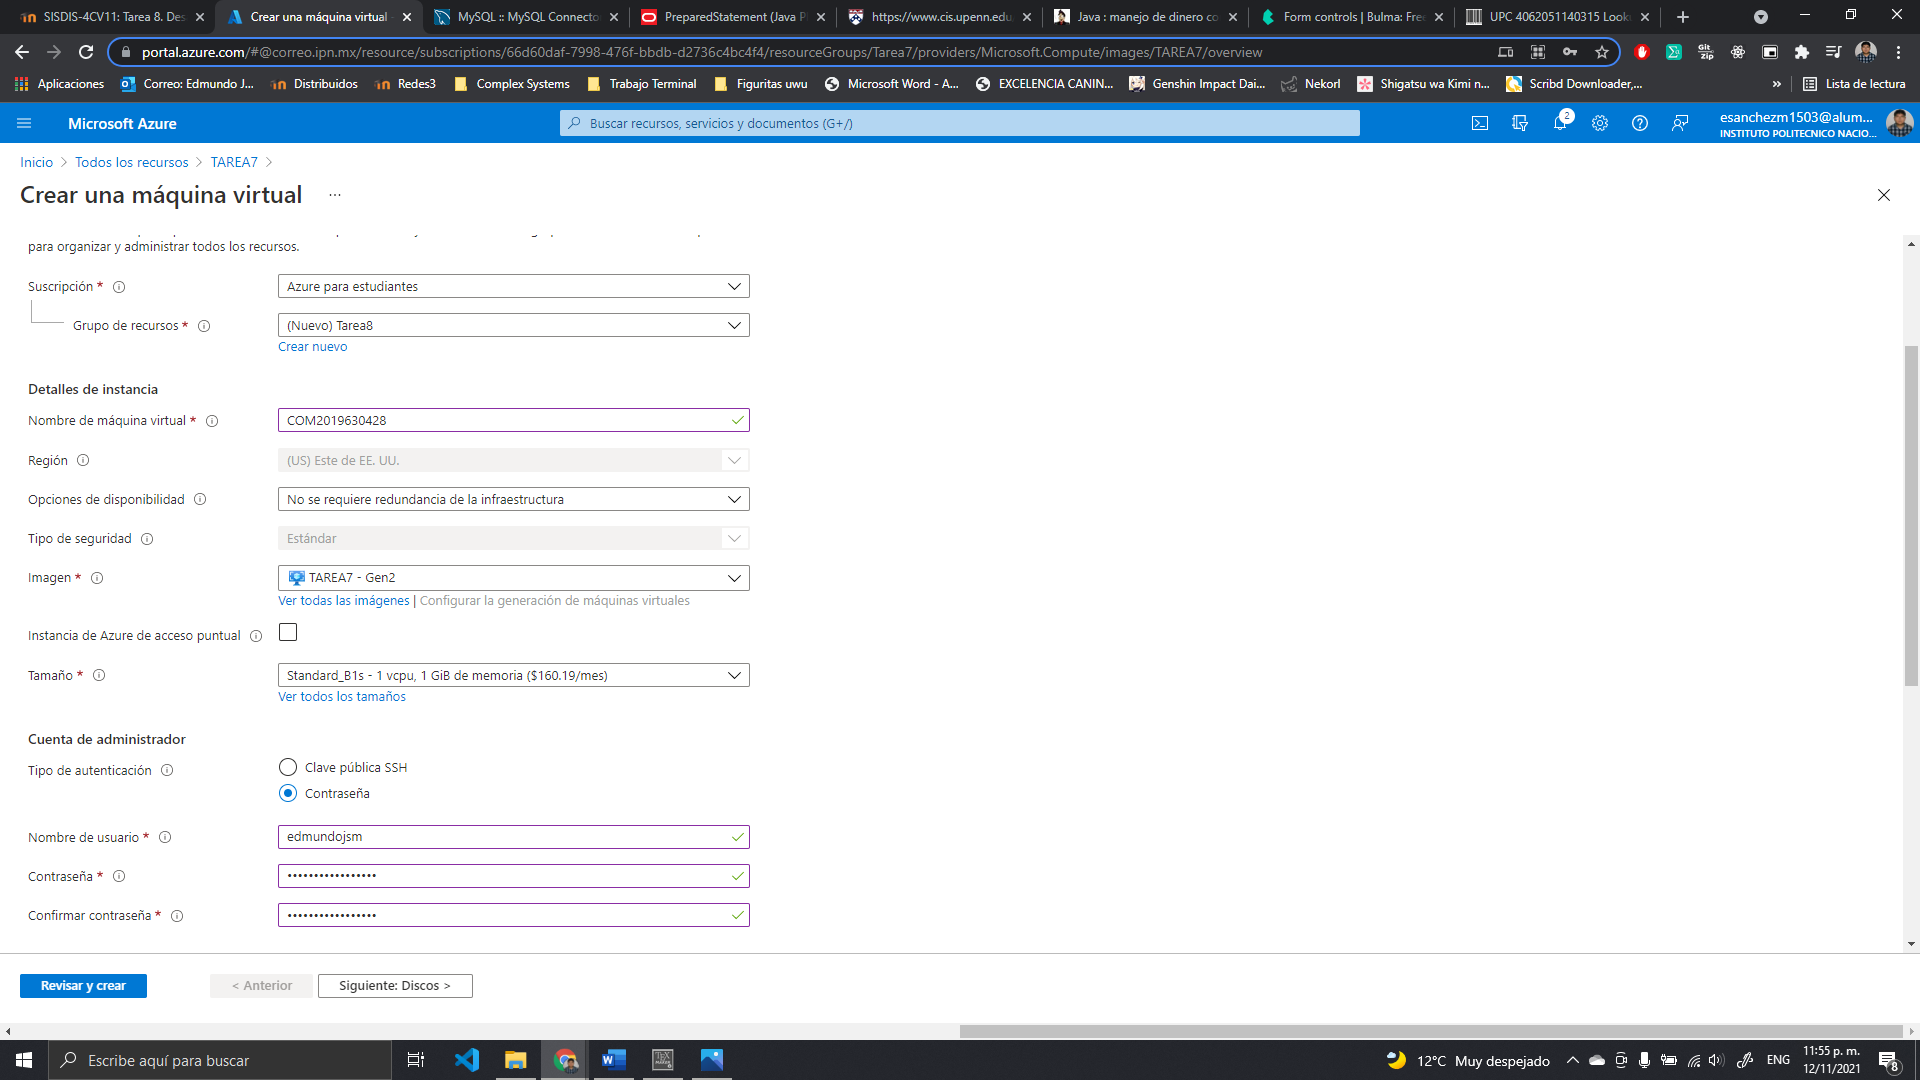
\includegraphics[scale=0.34]{resources/Infobasica.png}
			\caption{Datos básicos de la maquina virtual.}\label{fig:picture}
		\end{figure}
		\begin{figure}[H]
			\centering
			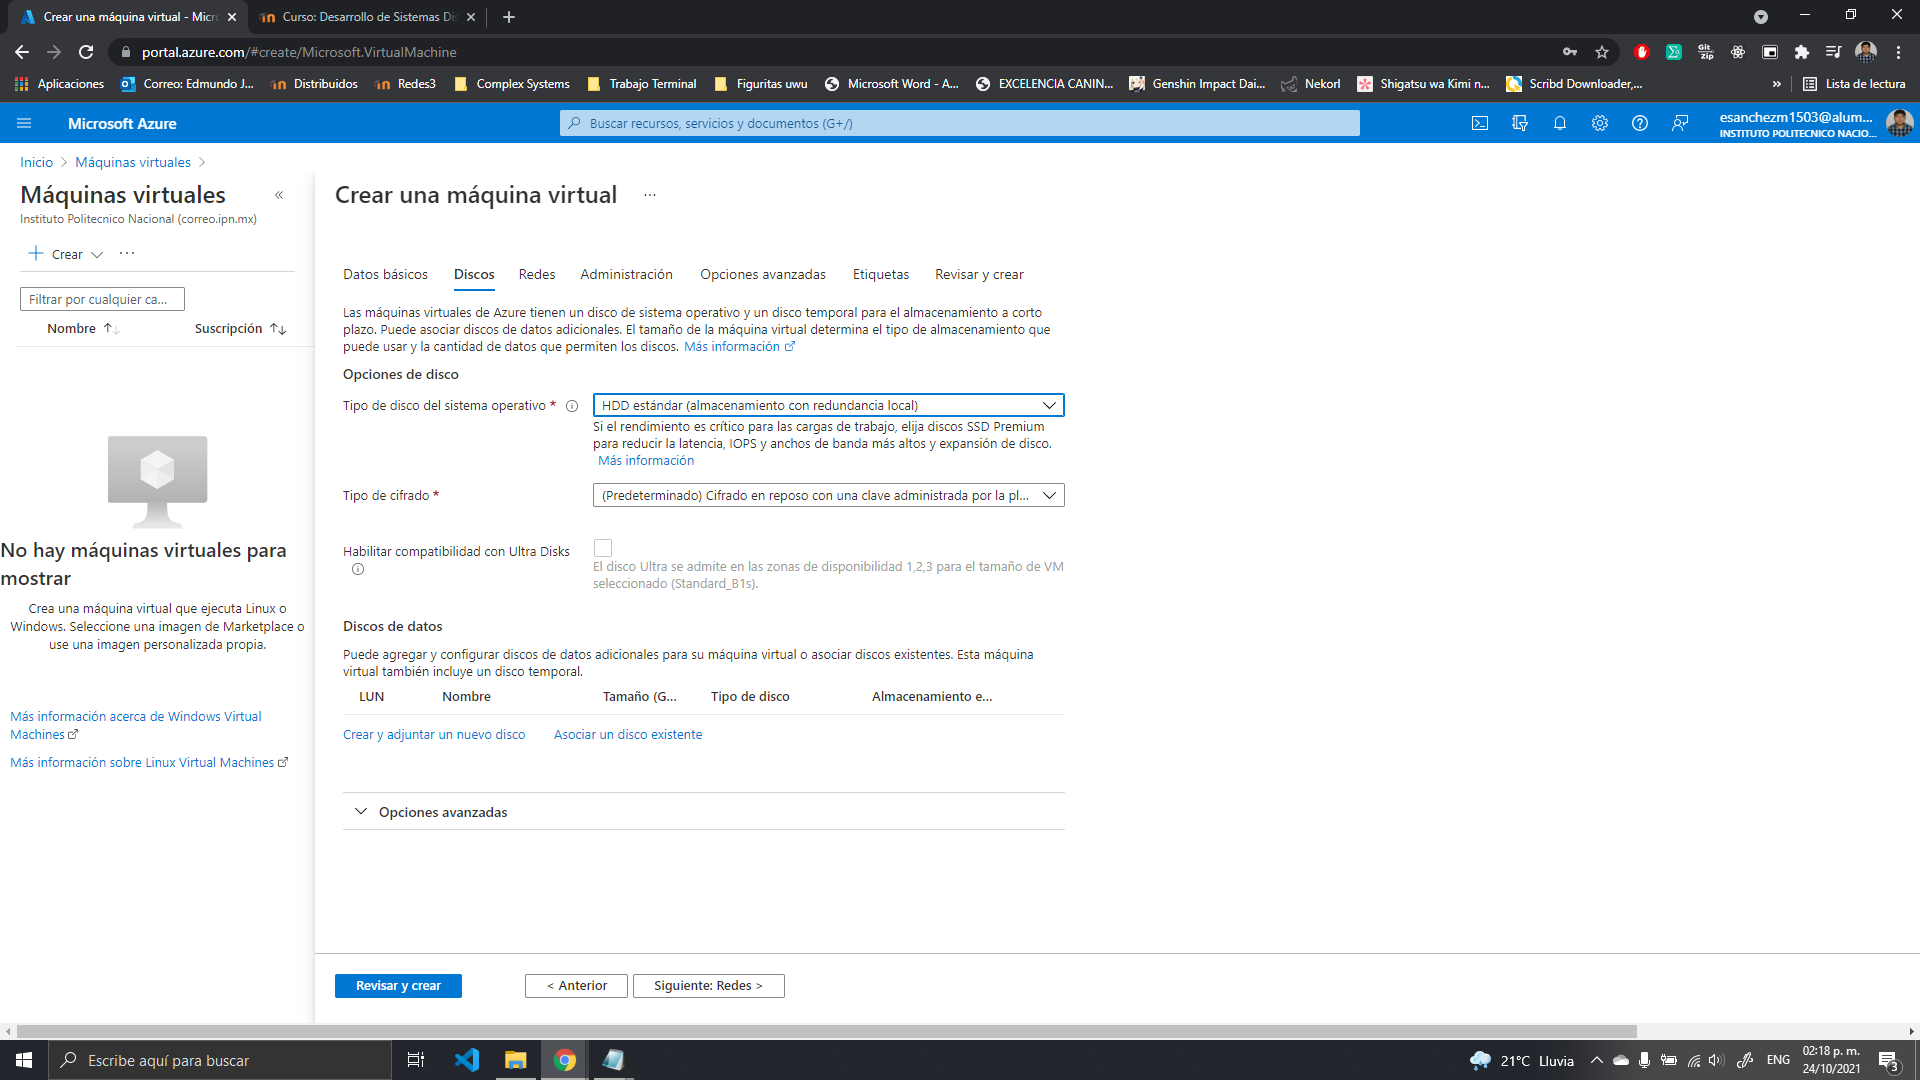
\includegraphics[scale=0.34]{resources/disco.png}
			\caption{Configuración del tipo de disco de la maquina virtual.}\label{fig:picture}
		\end{figure}
		\begin{figure}[H]
			\centering
			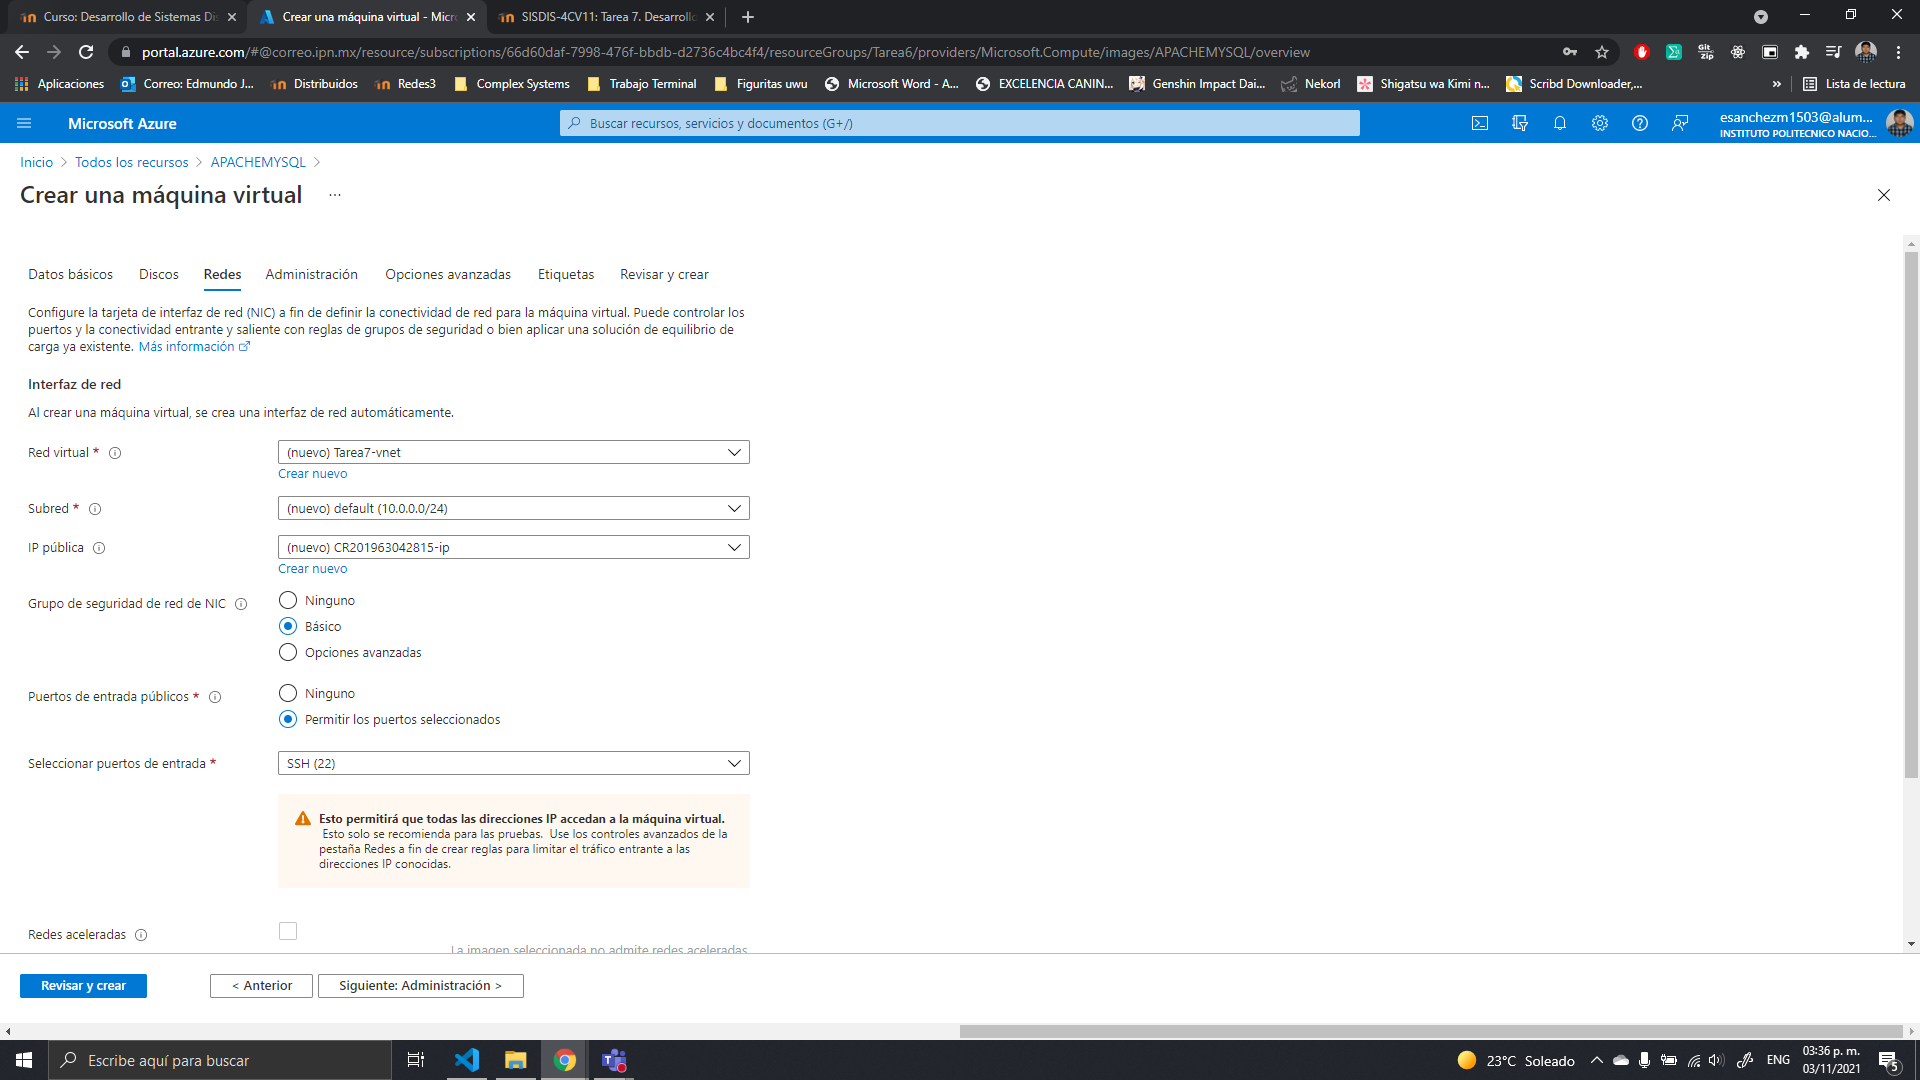
\includegraphics[scale=0.34]{resources/redes.png}
			\caption{Información sobre la redes de la maquina virtual.}\label{fig:picture}
		\end{figure}
		\begin{figure}[H]
			\centering
			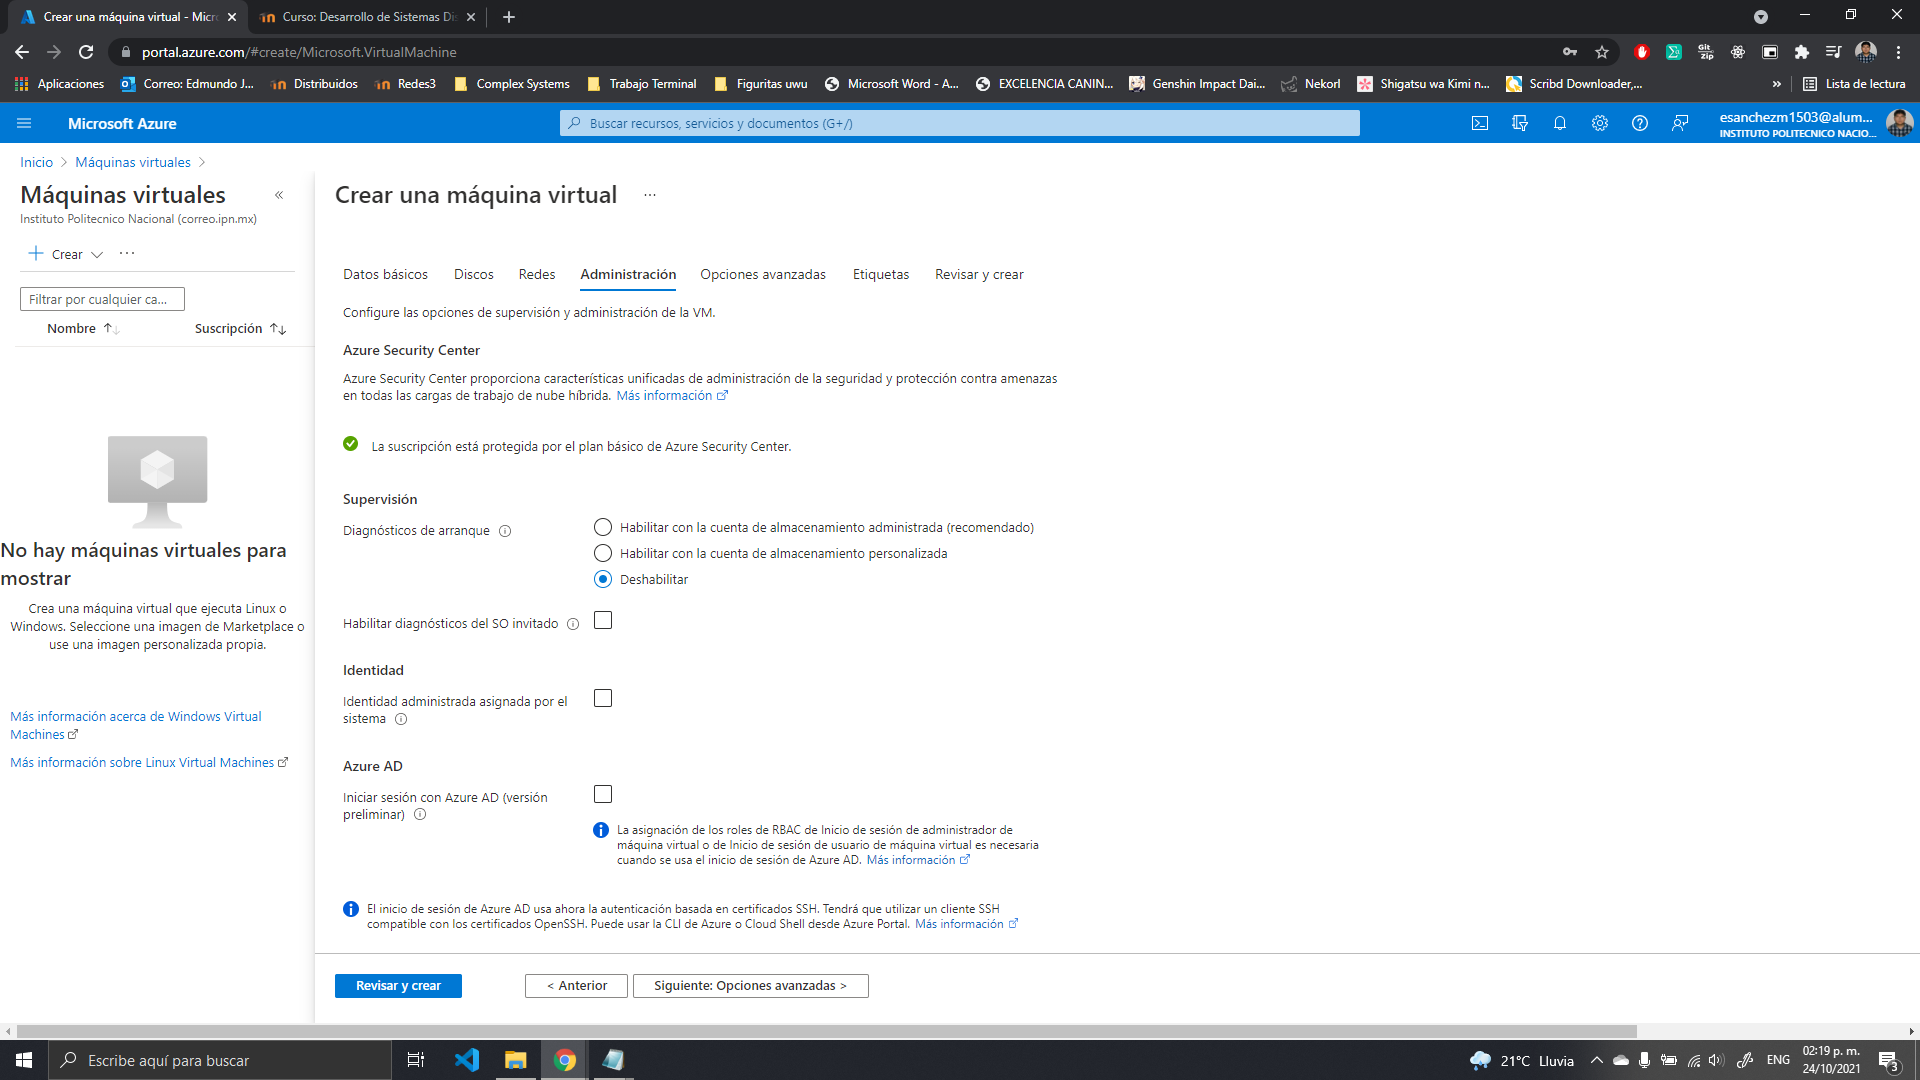
\includegraphics[scale=0.34]{resources/admin.png}
			\caption{Configuración de la administración de la maquina virtual.}\label{fig:picture}
		\end{figure}
		\begin{figure}[H]
			\centering
			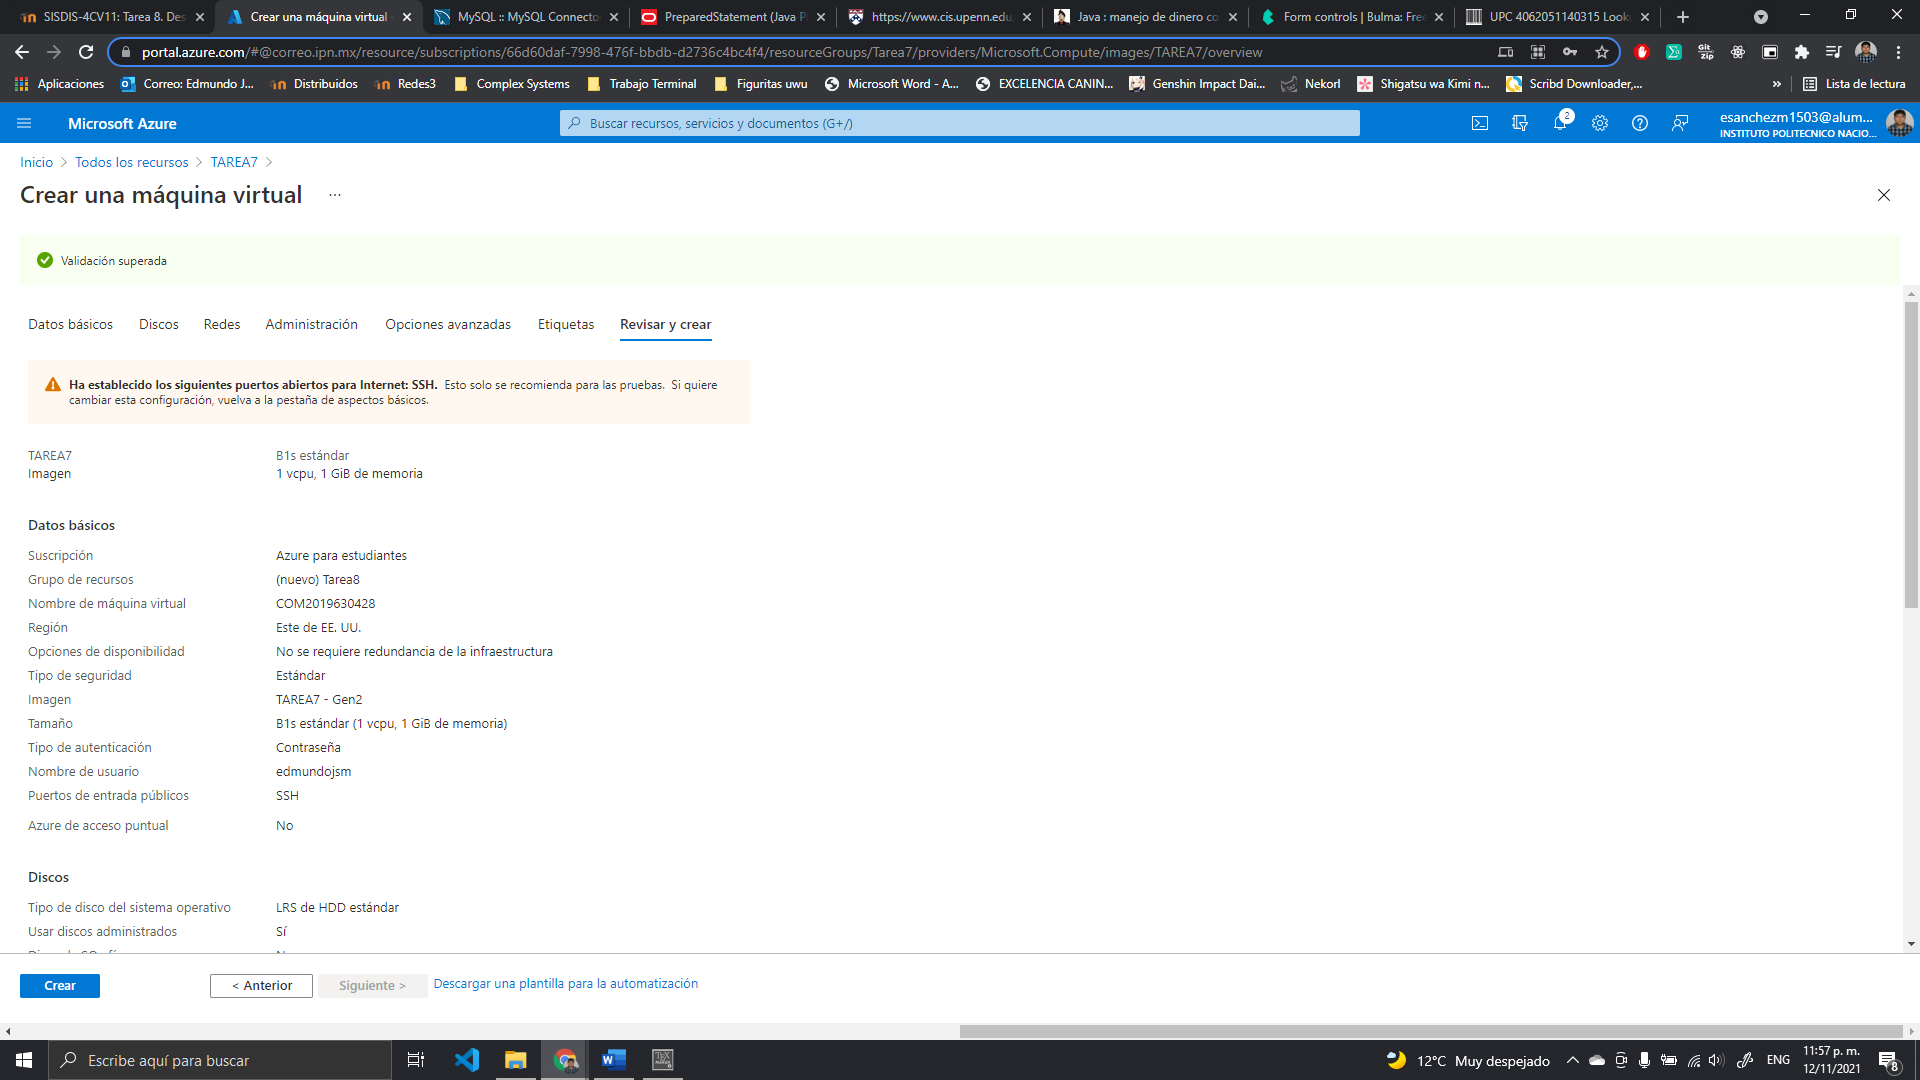
\includegraphics[scale=0.34]{resources/revisarycrear.png}
			\caption{Creación de la maquina virtual.}\label{fig:picture}
		\end{figure}
		\begin{figure}[H]
			\centering
			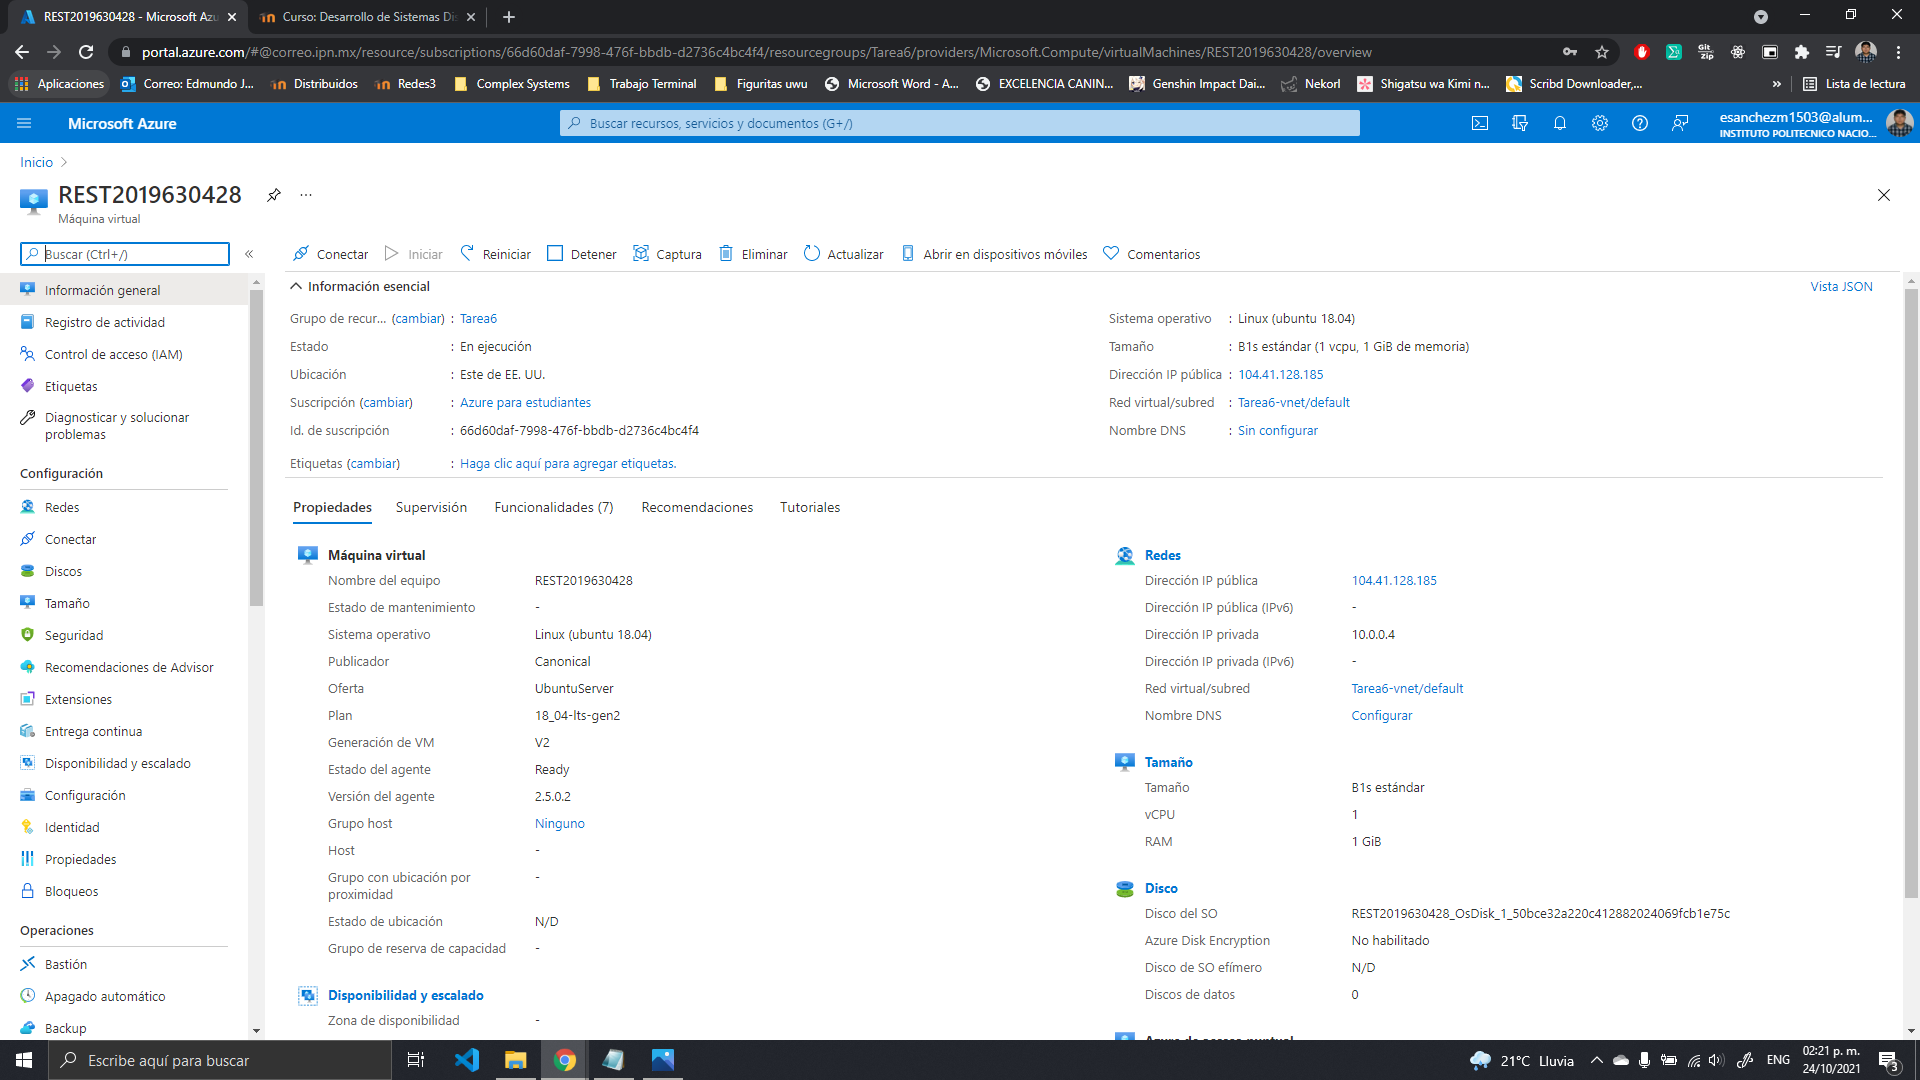
\includegraphics[scale=0.34]{resources/paneldecontrol.png}
			\caption{Panel de control de la maquina virtual.}\label{fig:picture}
		\end{figure}
		Una vez creada la maquina virtual tenemos que abrir el puerto 8080, ya que este puerto es el que ocupa Apache Tomcat, así podemos conectarnos de manera remota desde cualquier dispositivo , también es importante mencionar que si no se configura de manera correcta el puerto 8080 la conexión con la maquina virtual para poder visualizar el servicio web. En las figuras 7 y 8 podemos ver la configuración del puerto.
		\begin{figure}[H]
			\centering
			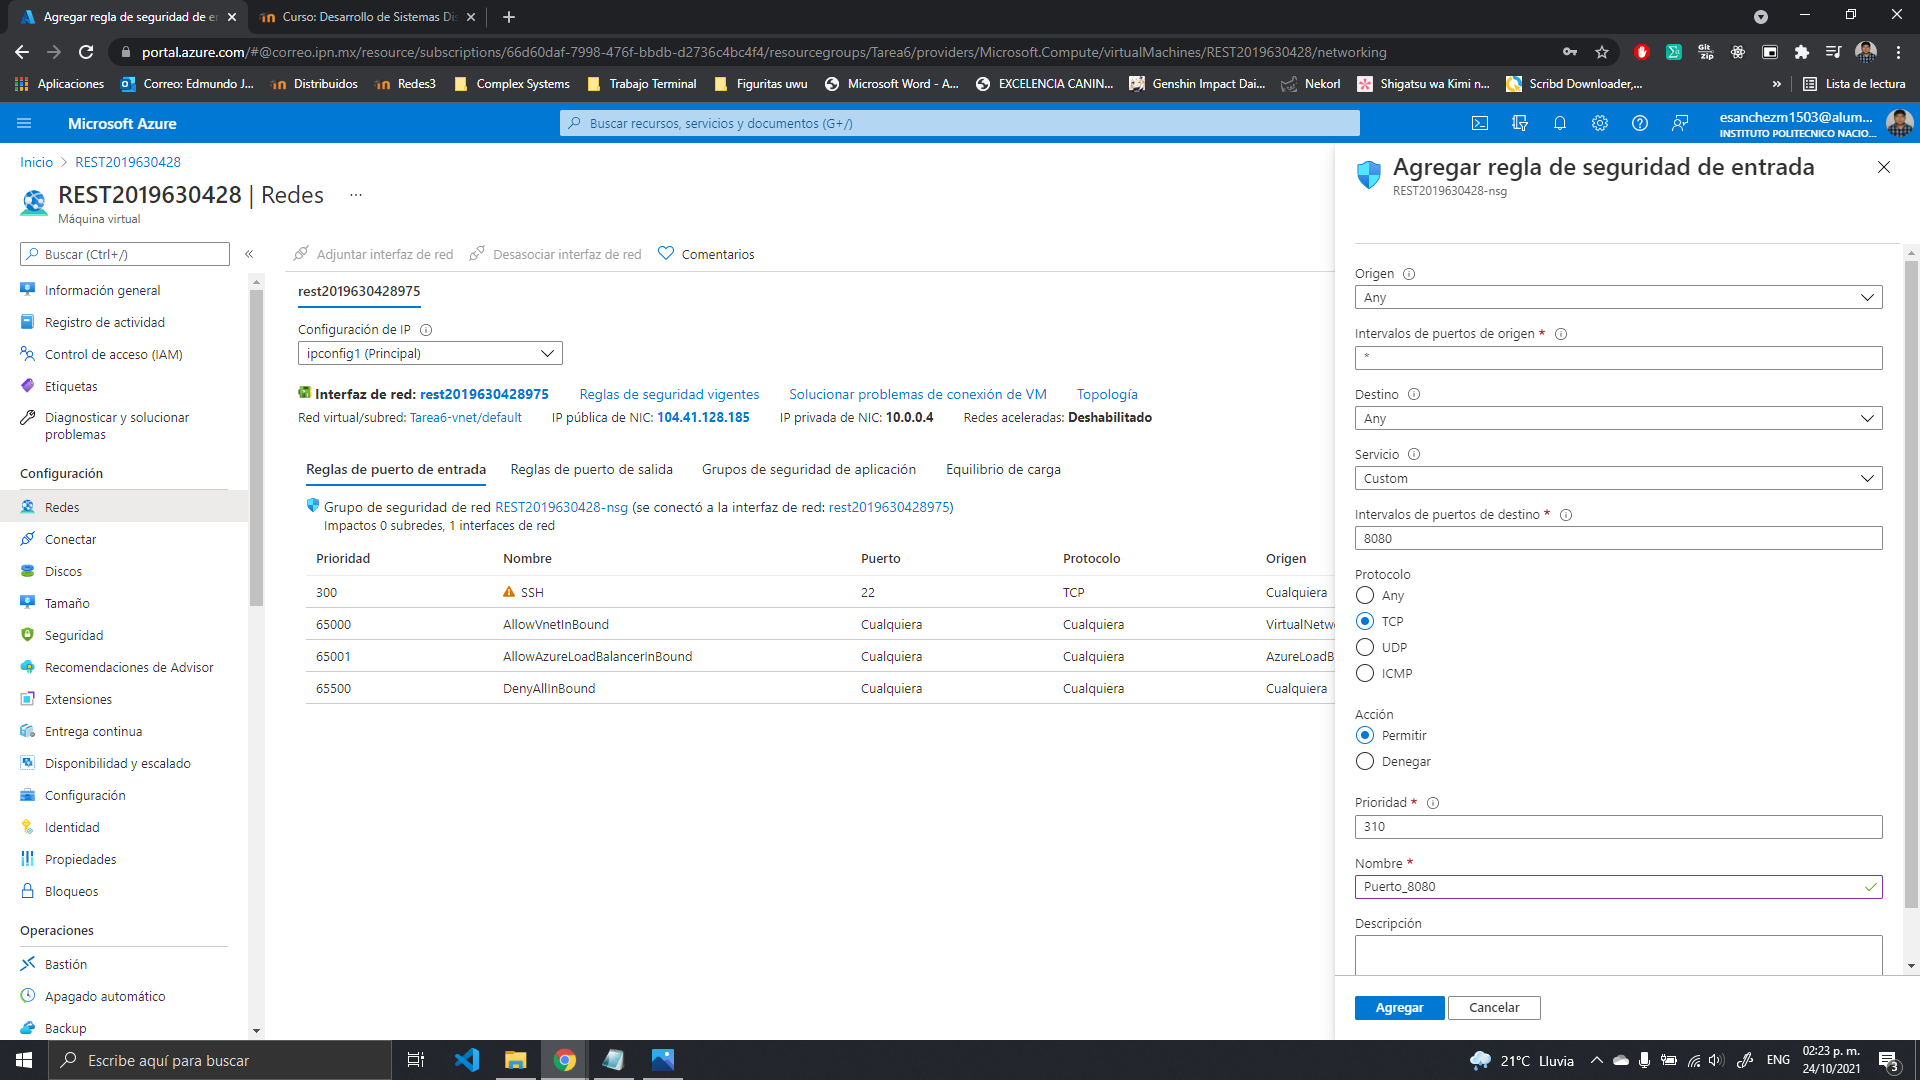
\includegraphics[scale=0.34]{resources/open8080.png}
			\caption{Configuración del puerto 8080.}\label{fig:picture}
		\end{figure}
		\begin{figure}[H]
			\centering
			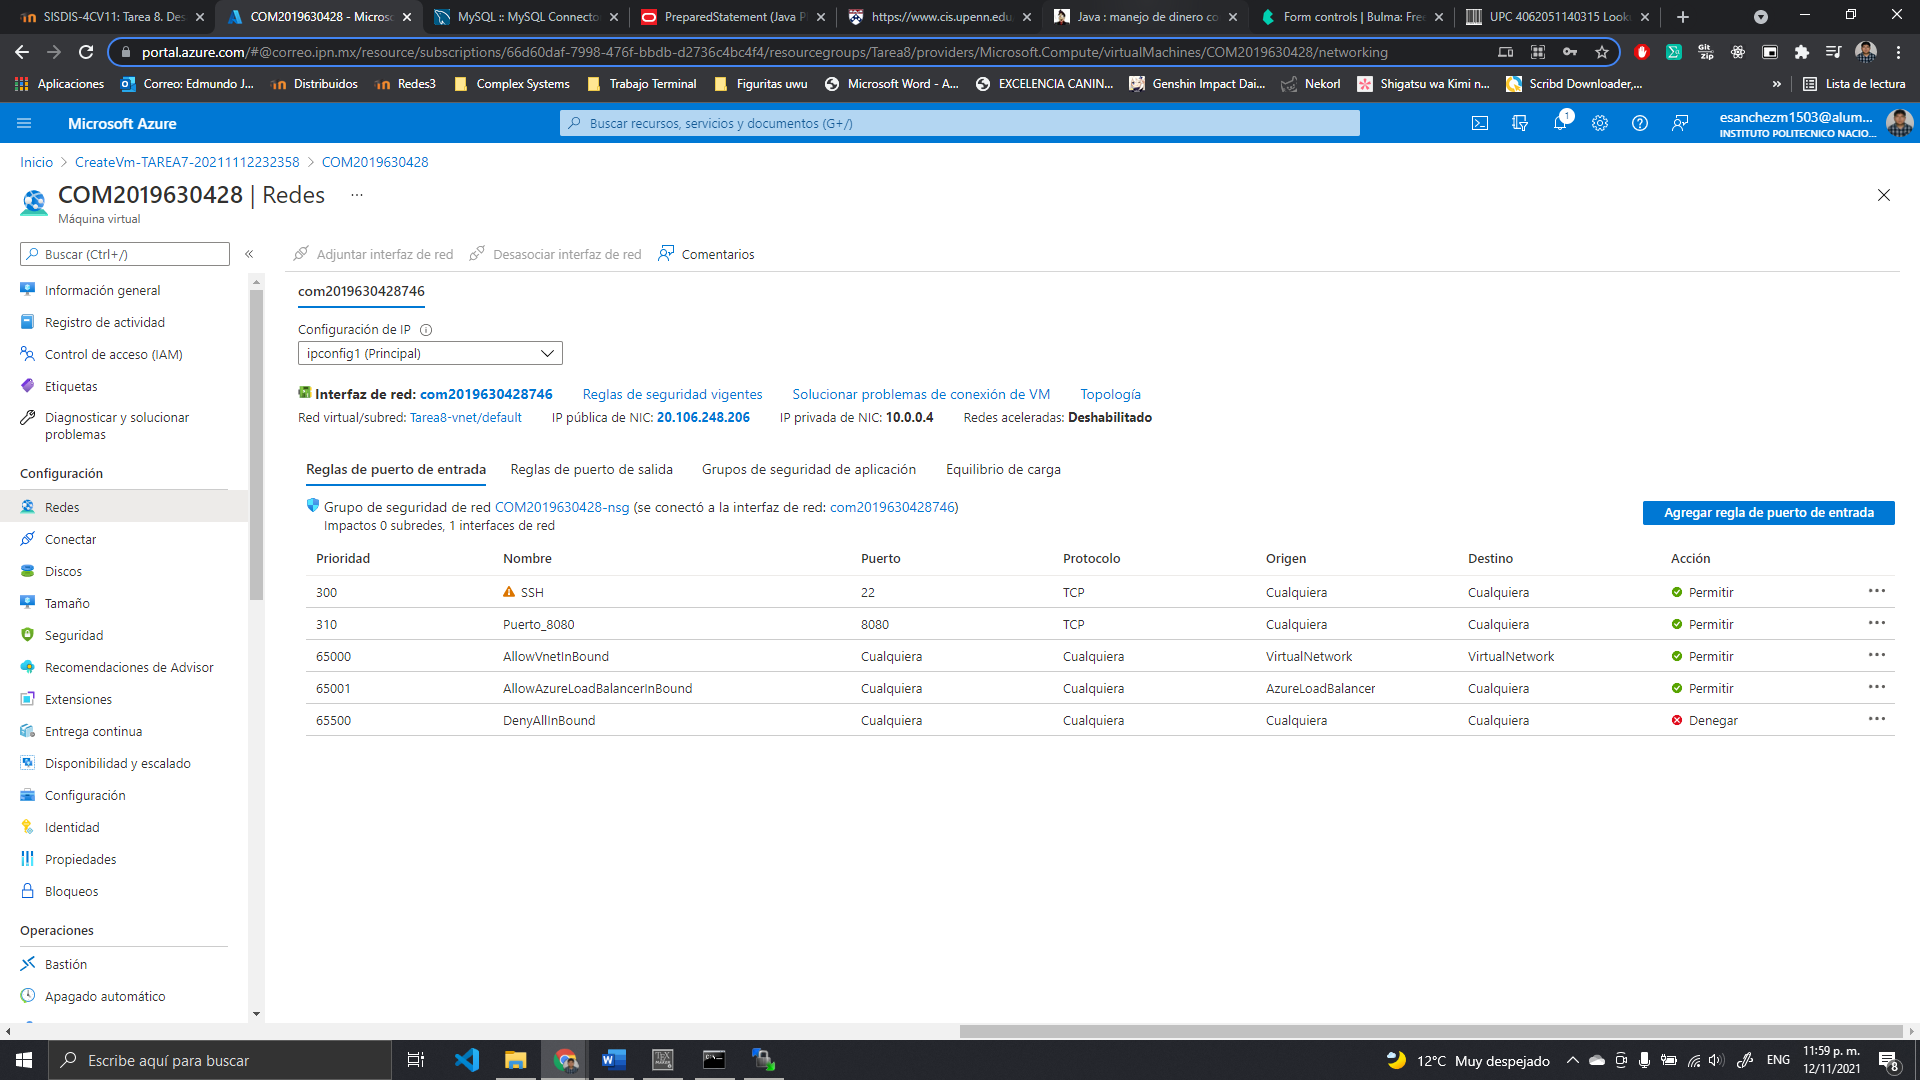
\includegraphics[scale=0.34]{resources/puertook.png}
			\caption{Puerto 8080 abierto correctamente.}\label{fig:picture}
		\end{figure}
		Ya teniendo la maquina preparada, procederemos al siguiente punto de la practica, el cual es la instalación de Tomcat con soporte REST
		\subsection{Instalación de Tomcat con soporte REST}
		Primero que nada nos tendremos que conectar por medio de ssh a la maquina virtual como vemos en la figura 9.
		\begin{figure}[H]
			\centering
			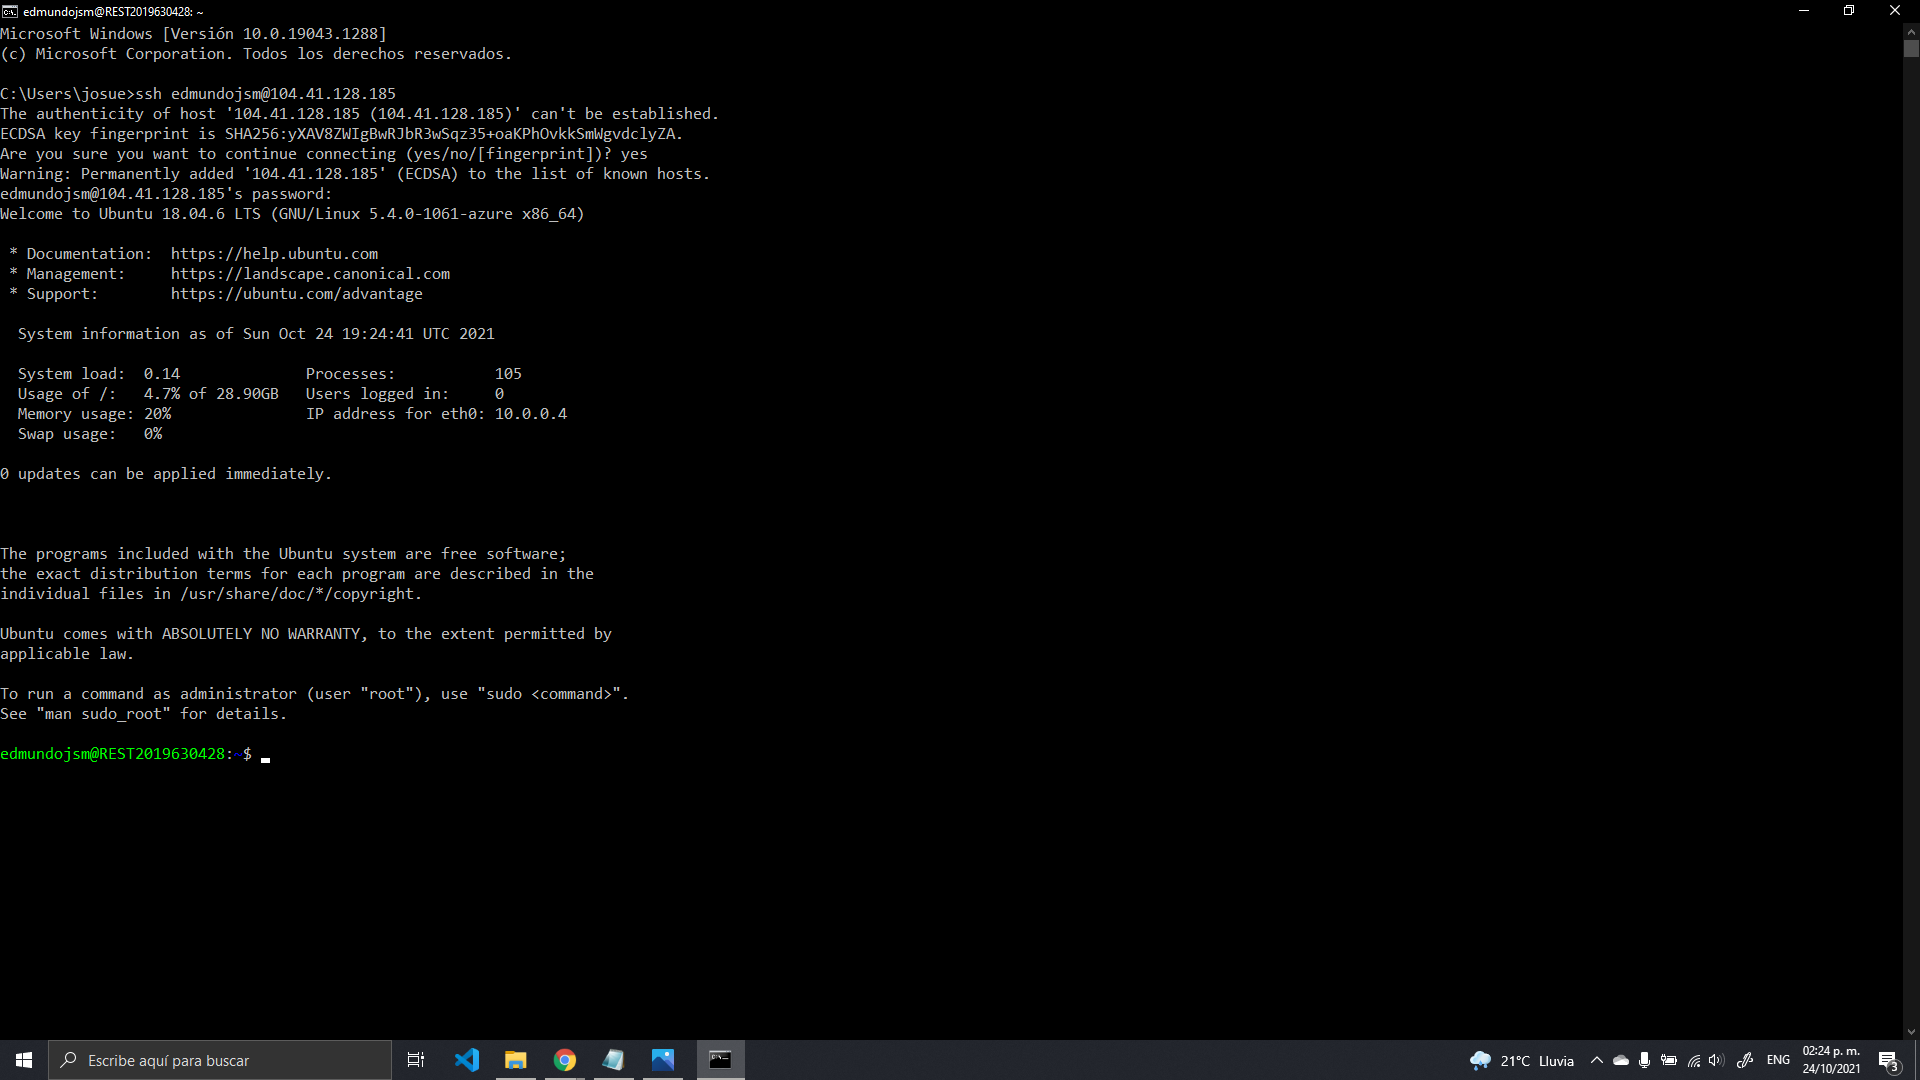
\includegraphics[scale=0.34]{resources/conexionssh.png}
			\caption{Conexión ssh con la maquina virtual.}\label{fig:picture}
		\end{figure}
		Posteriormente instalamos el JDK8 en la maquina virtual, como se ve en las figuras 10 y 11.
		\begin{figure}[H]
			\centering
			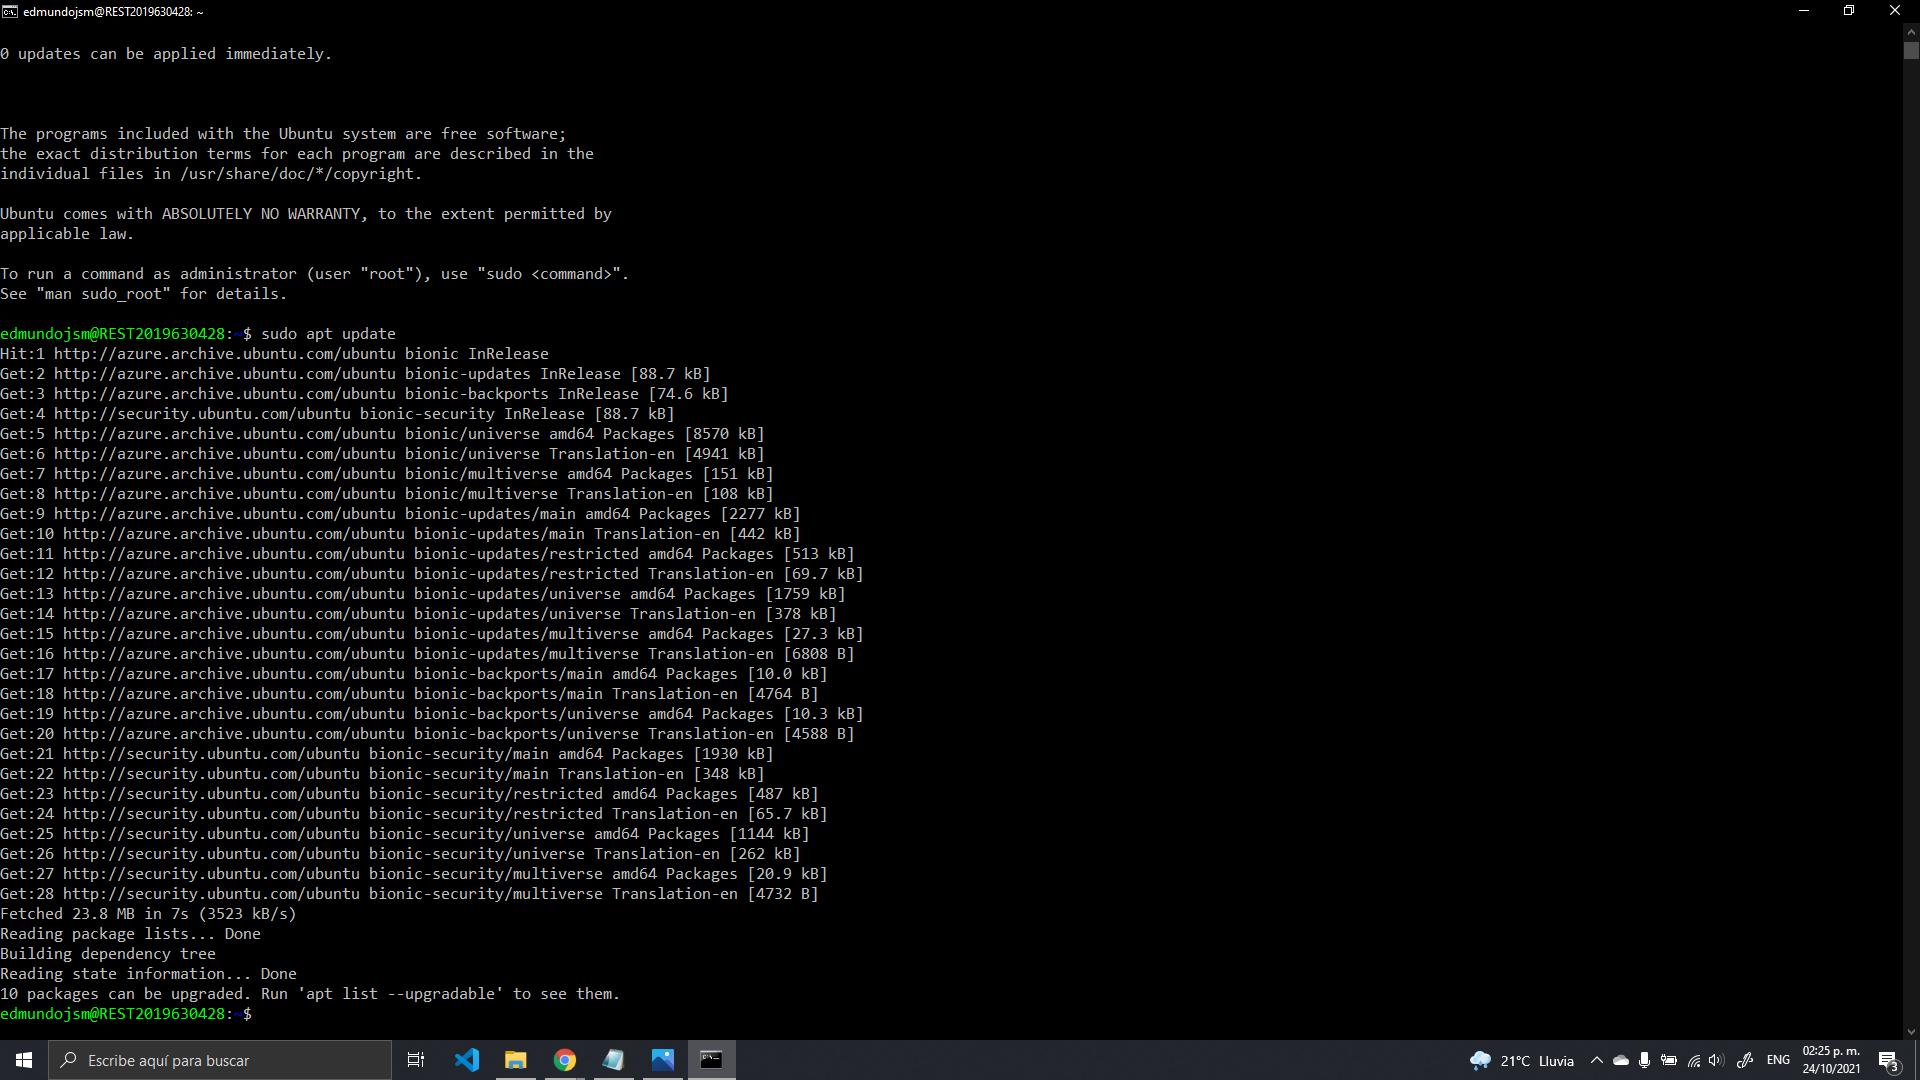
\includegraphics[scale=0.34]{resources/p2.1.png}
			\caption{Ejecución del comando sudo apt update.}\label{fig:picture}
		\end{figure}
		\begin{figure}[H]
			\centering
			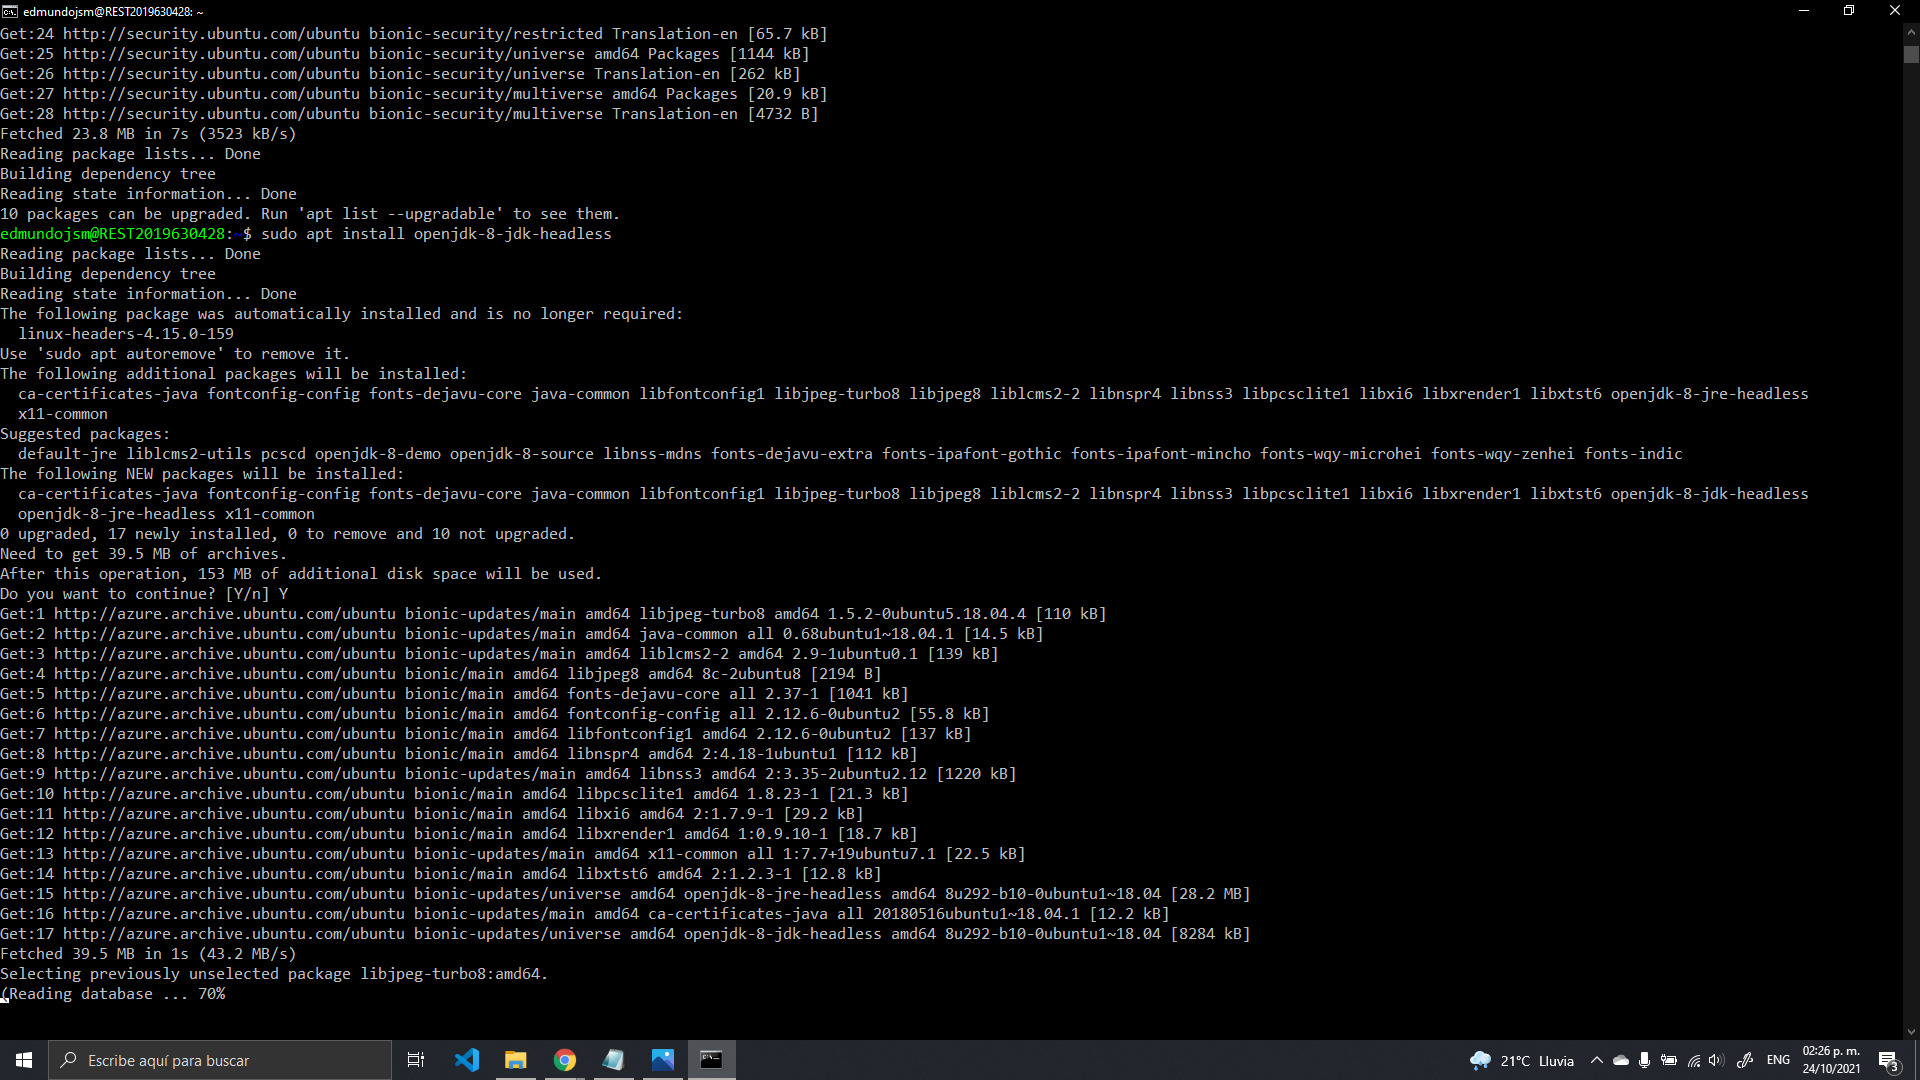
\includegraphics[scale=0.34]{resources/p2.2.png}
			\caption{Ejecución del comando sudo apt install openjdk-8-jdk-headless.}	\label{fig:picture}
		\end{figure}
		Después llevamos acabo lo que vemos en las figuras 12 a la 25, en estos pasos preparamos Tomcat para su uso posterior.
		\begin{figure}[H]
			\centering
			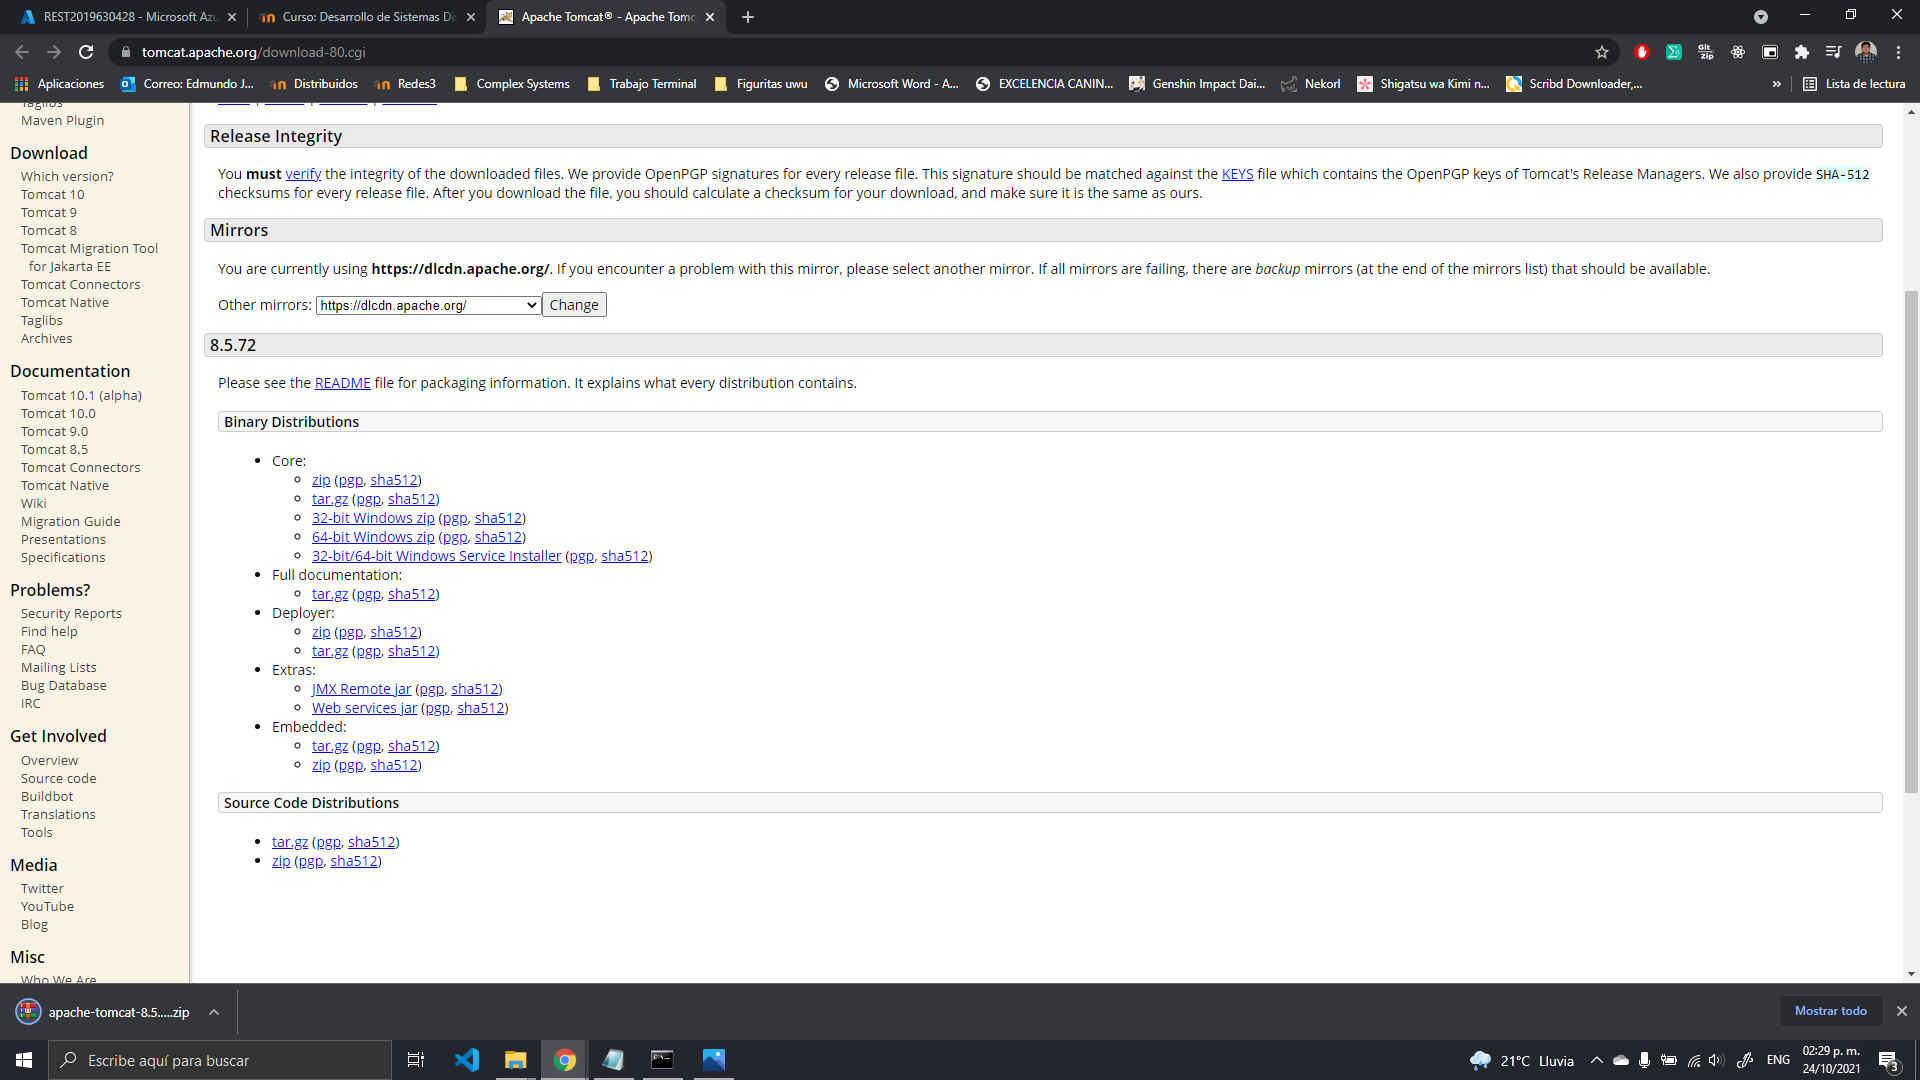
\includegraphics[scale=0.34]{resources/p3.png}
			\caption{Descargamos la distribución binaria de Tomcat 8 en ZIP de la siguiente URL https://tomcat.apache.org/download-80.cgi.}\label{fig:picture}
		\end{figure}
		\begin{figure}[H]
			\centering
			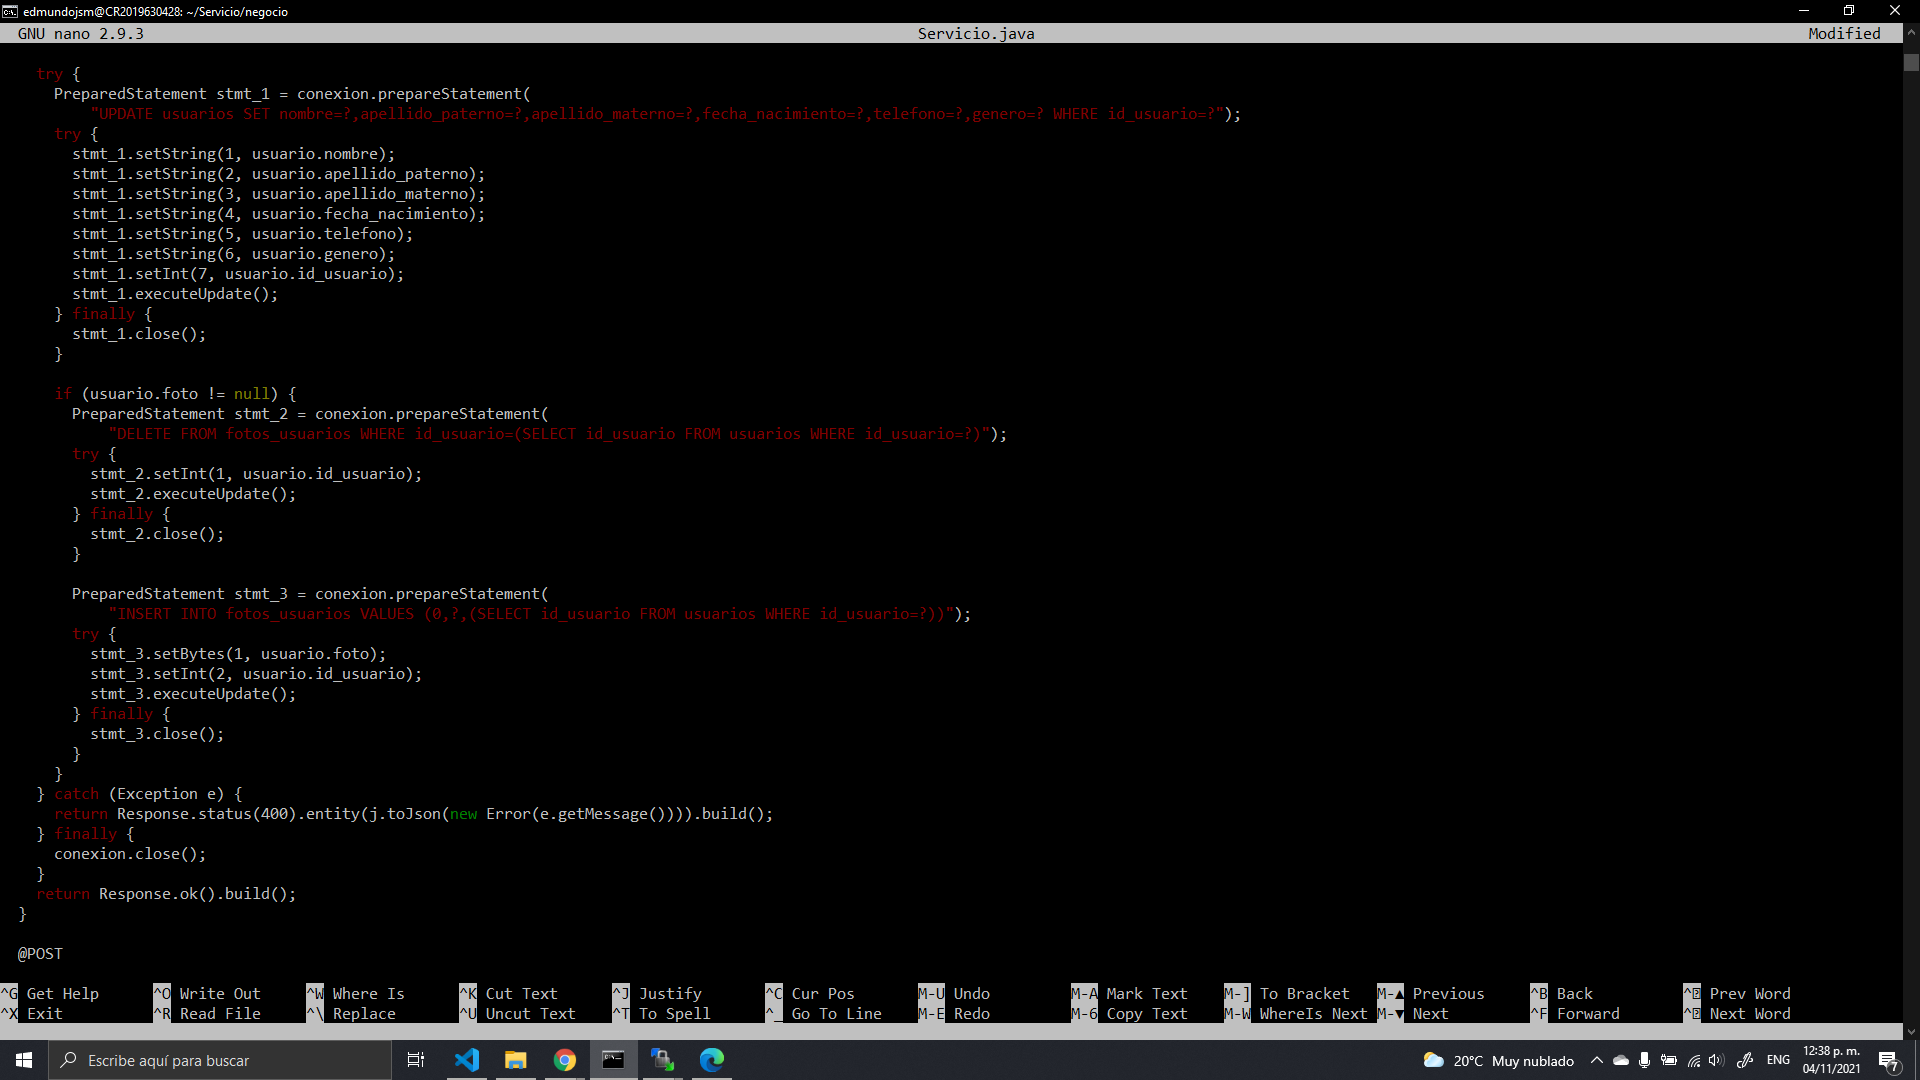
\includegraphics[scale=0.34]{resources/p4.1.png}
			\caption{Copiamos a la máquina virtual el archivo ZIP descargado.}\label{fig:picture}
		\end{figure}
		\begin{figure}[H]
			\centering
			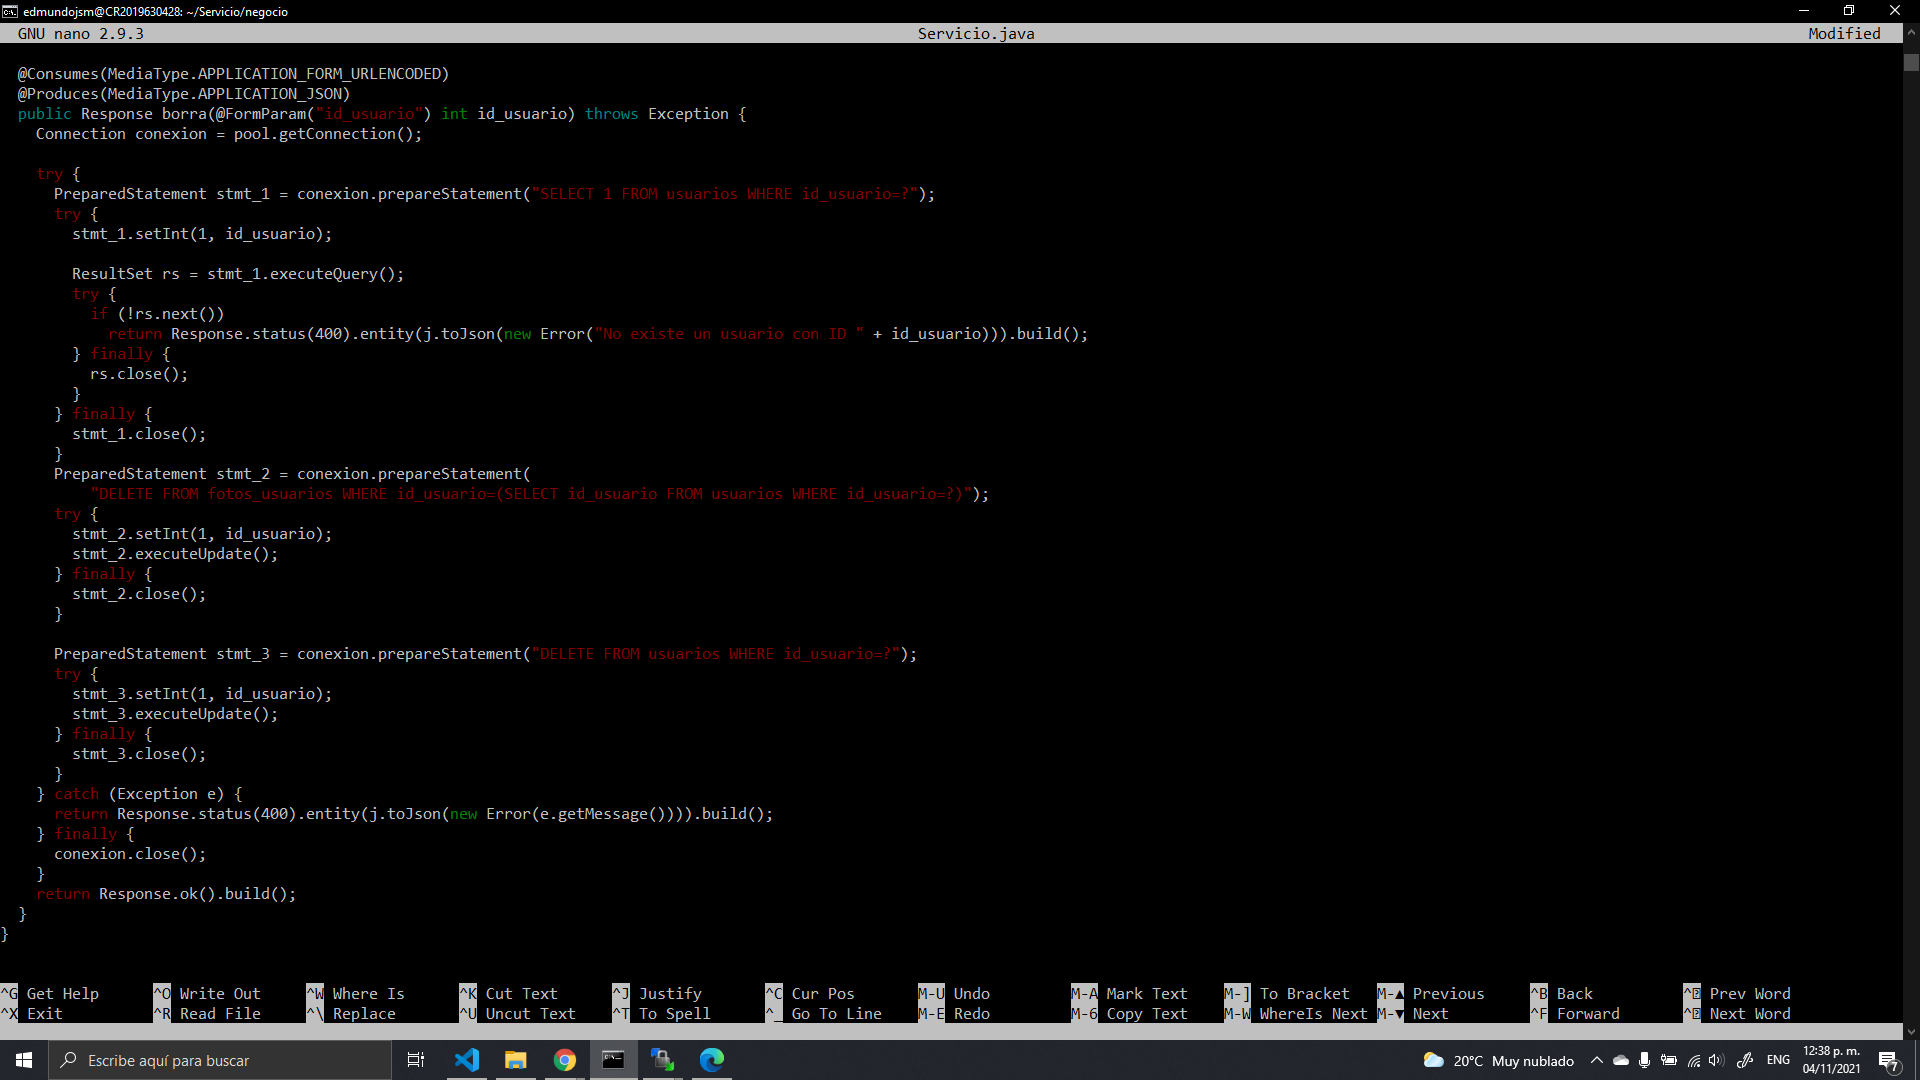
\includegraphics[scale=0.34]{resources/p5.png}
			\caption{Eliminamos el directorio webapps el cual se encuentra dentro del directorio de Tomcat, ademas creamos un nuevo directorio webapps y dentro de éste se crea el directorio ROOT.}\label{fig:picture}
		\end{figure}
		\begin{figure}[H]
			\centering
			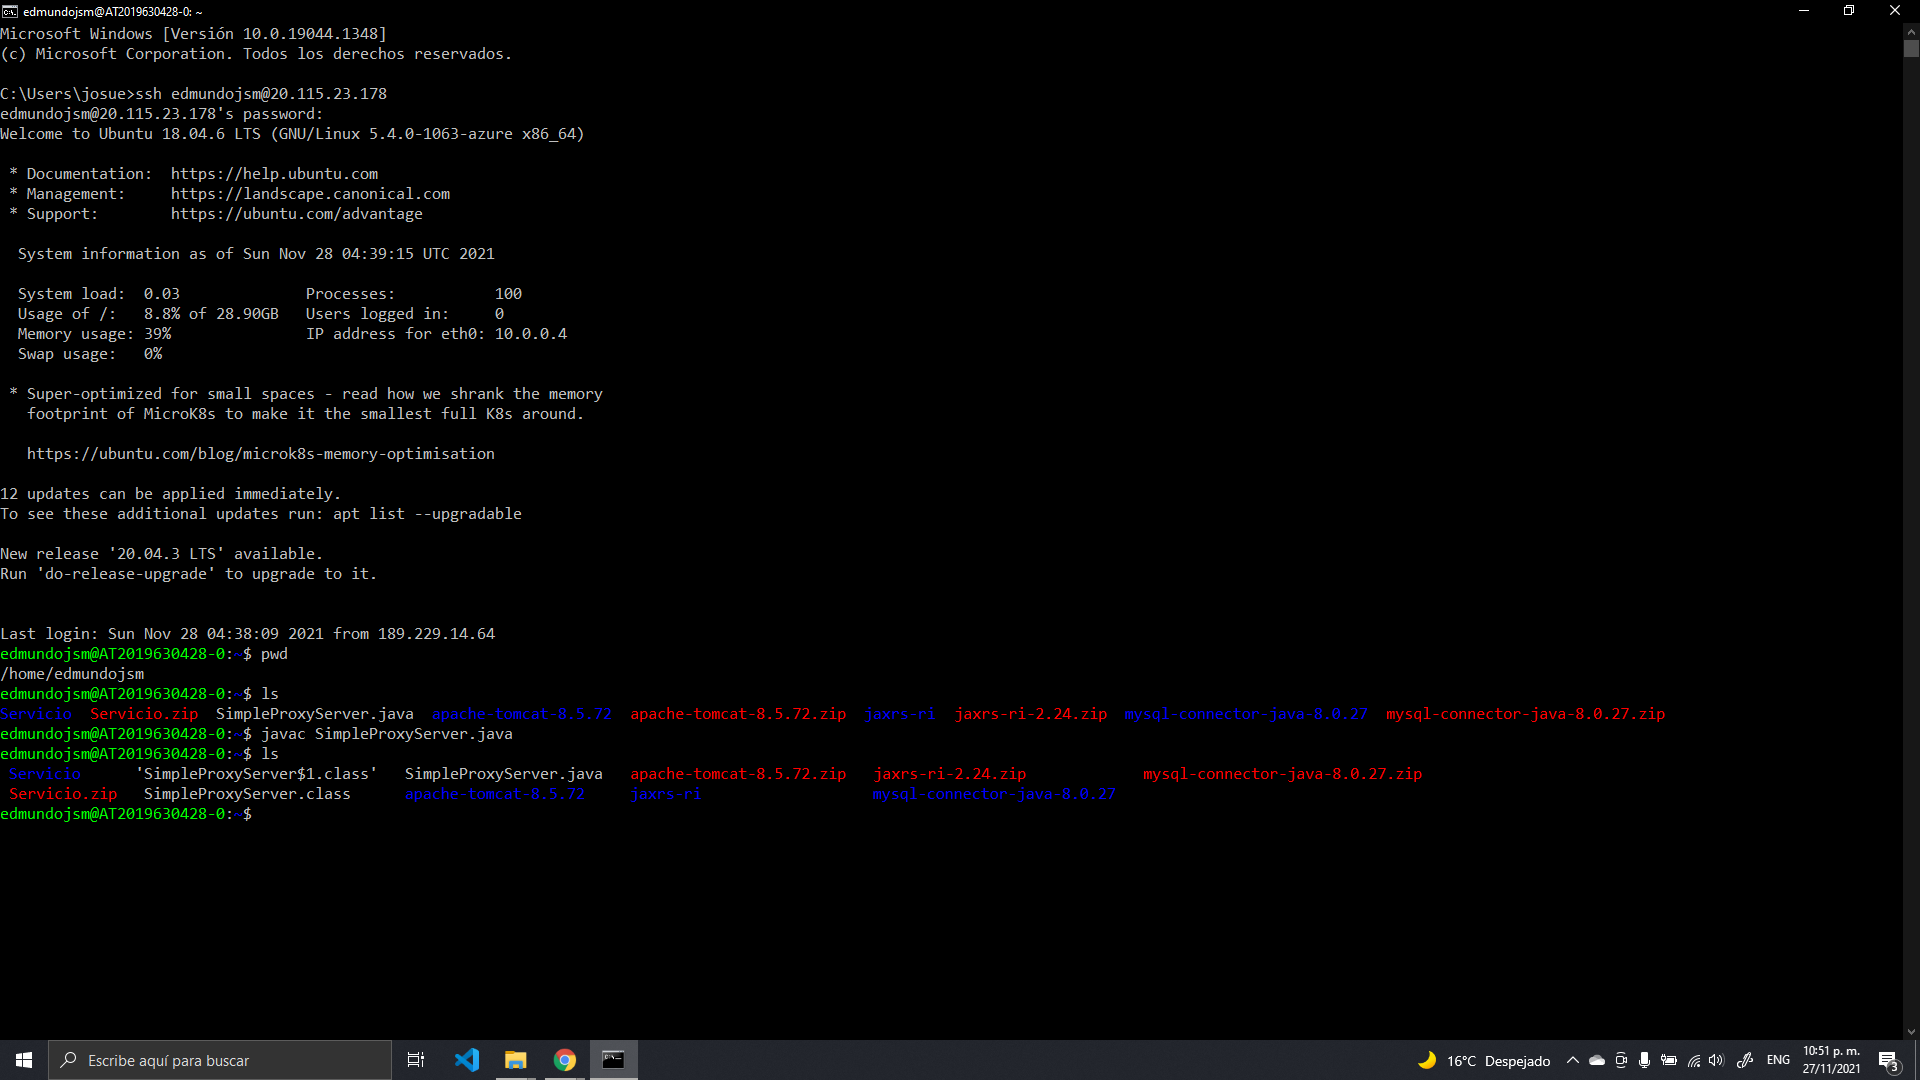
\includegraphics[scale=0.34]{resources/p6.png}
			\caption{Descargamos la biblioteca "Jersey" de la siguiente URL https://repo1.maven.org/maven2/org/glassfish/jersey/bundles/jaxrs-ri/2.24/jaxrs-ri-2.24.zip
.}\label{fig:picture}
		\end{figure}
		\begin{figure}[H]
			\centering
			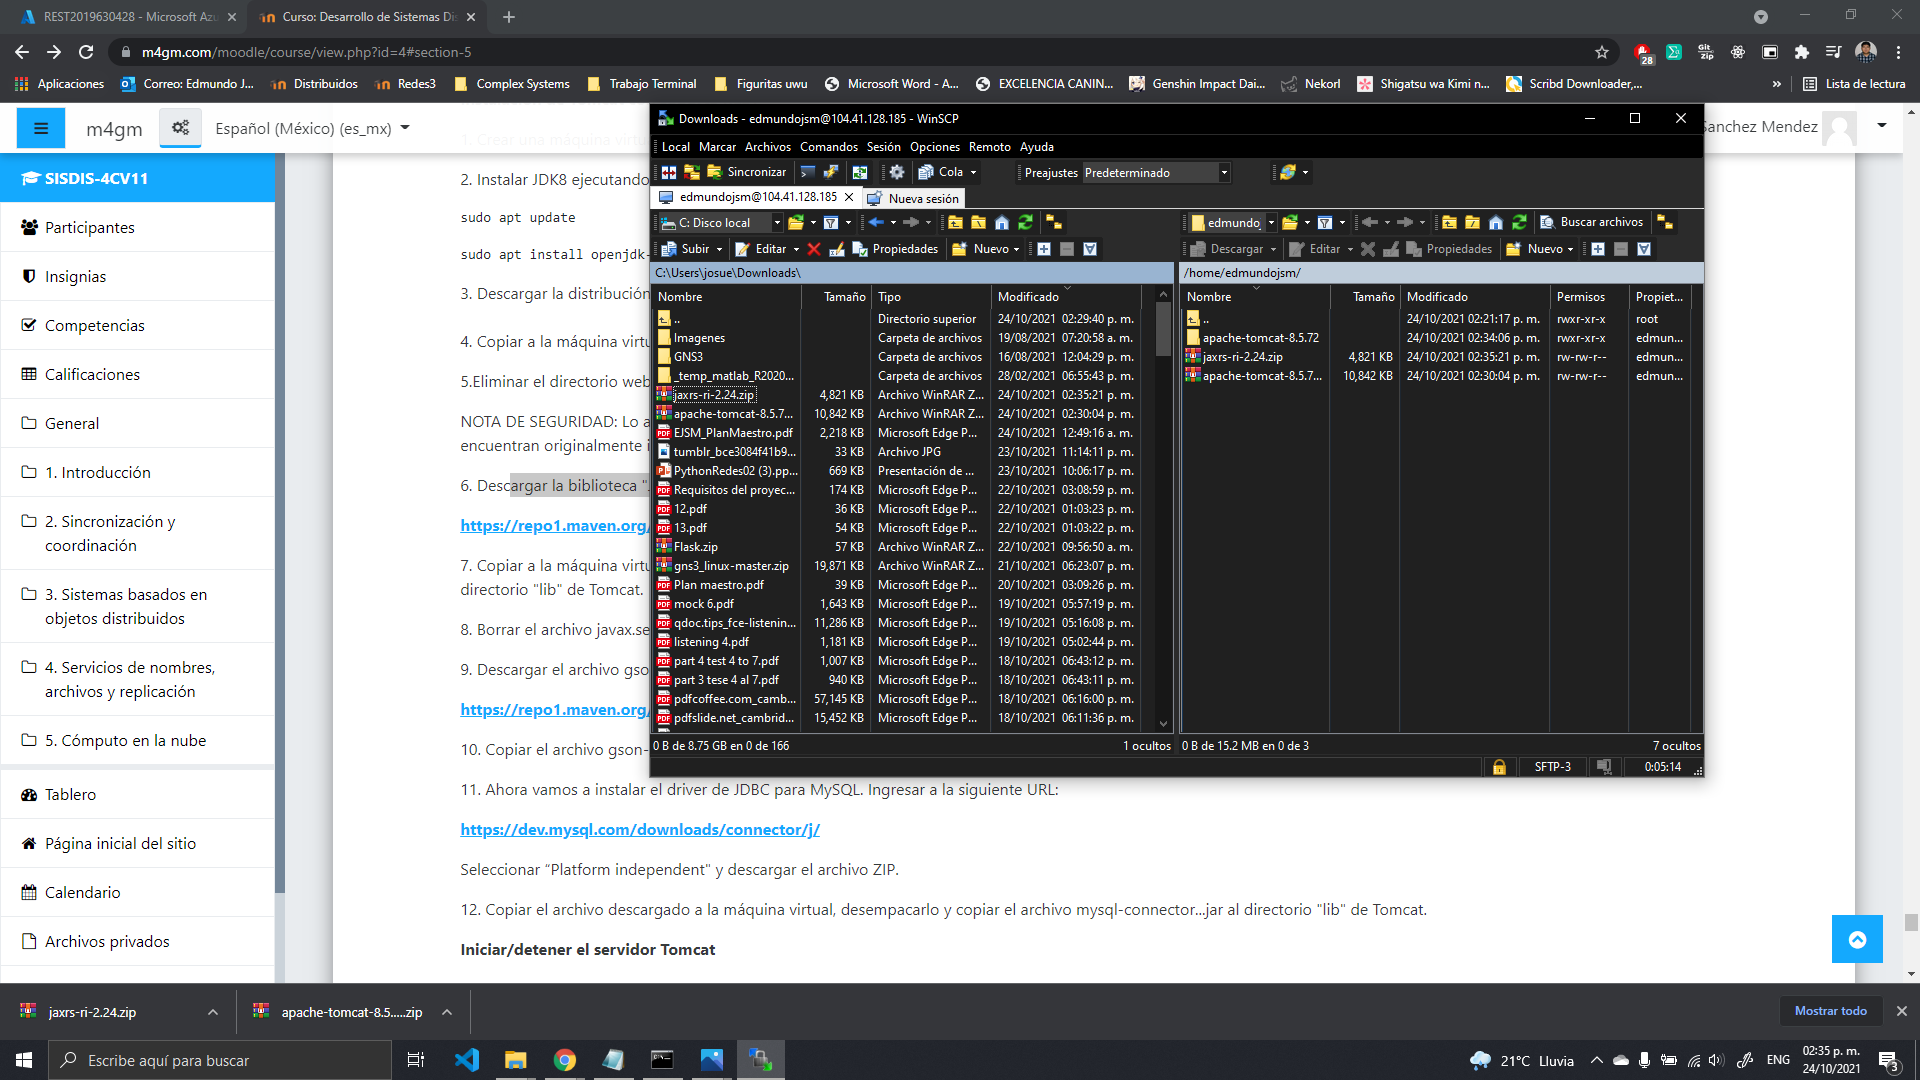
\includegraphics[scale=0.34]{resources/p7.1.png}
			\caption{Copiamos a la máquina virtual el archivo descargado en la figura anterior.}\label{fig:picture}
		\end{figure}
		\begin{figure}[H]
			\centering
			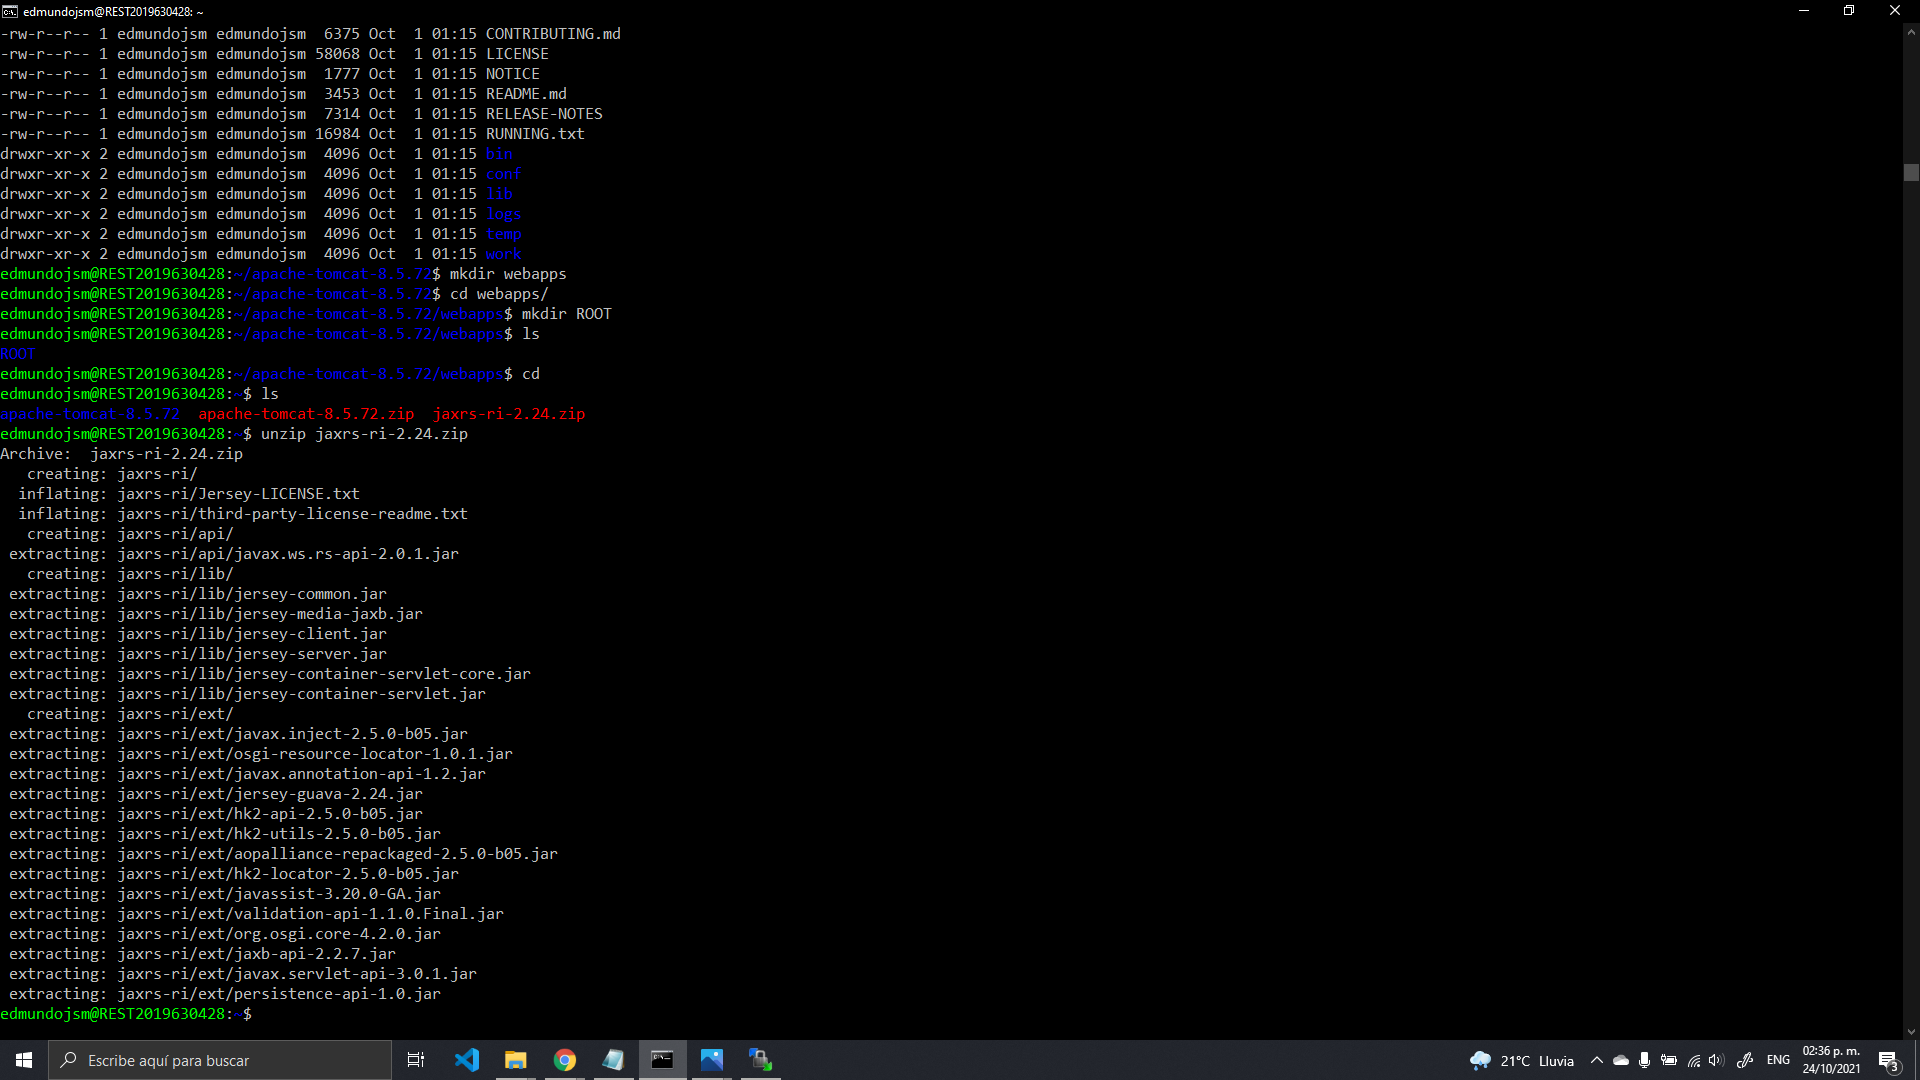
\includegraphics[scale=0.34]{resources/p7.2.png}
			\caption{Desempaquetamos el .zip de la figura anterior.}\label{fig:picture}
		\end{figure}
		\begin{figure}[H]
			\centering
			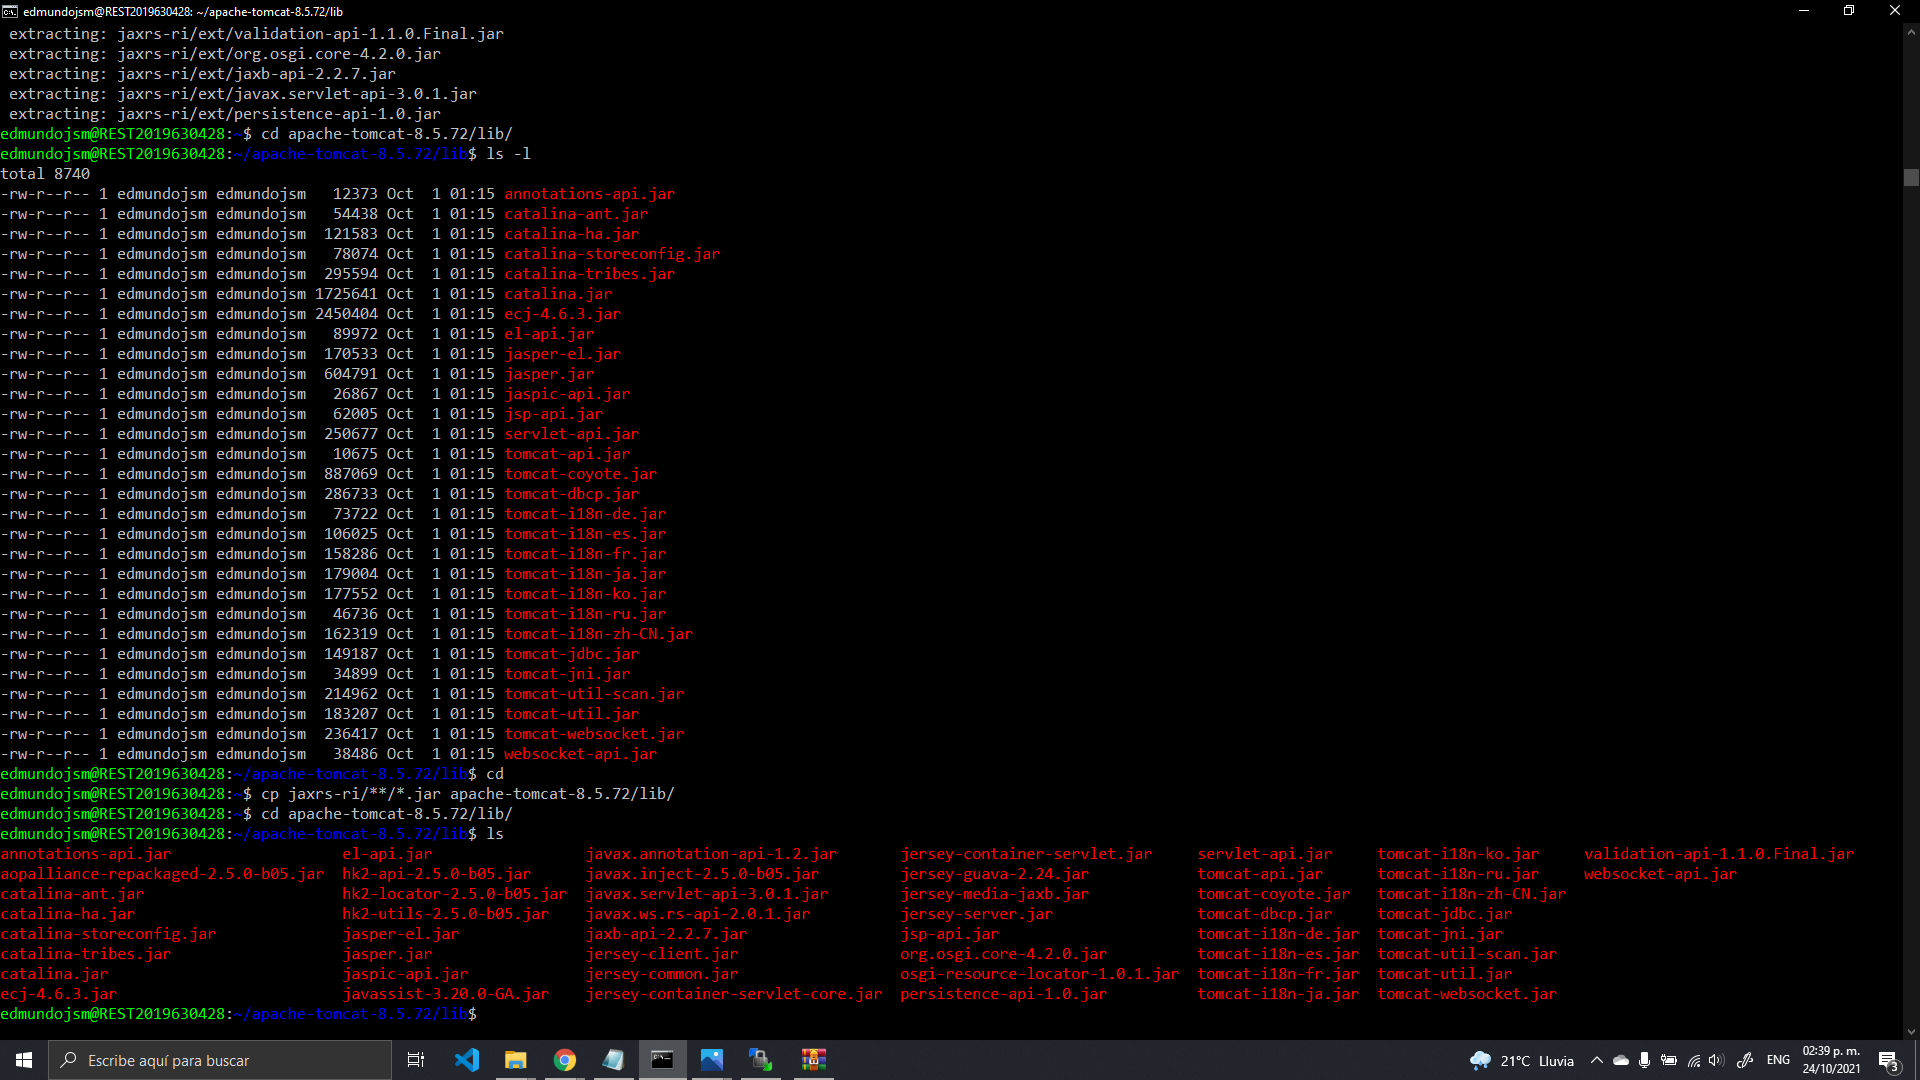
\includegraphics[scale=0.34]{resources/p7.3.png}
			\caption{Copiamos todos los archivos con extensión “.jar” de todos los directorios desempacados, al directorio "lib" de Tomcat.}\label{fig:picture}
		\end{figure}
		\begin{figure}[H]
			\centering
			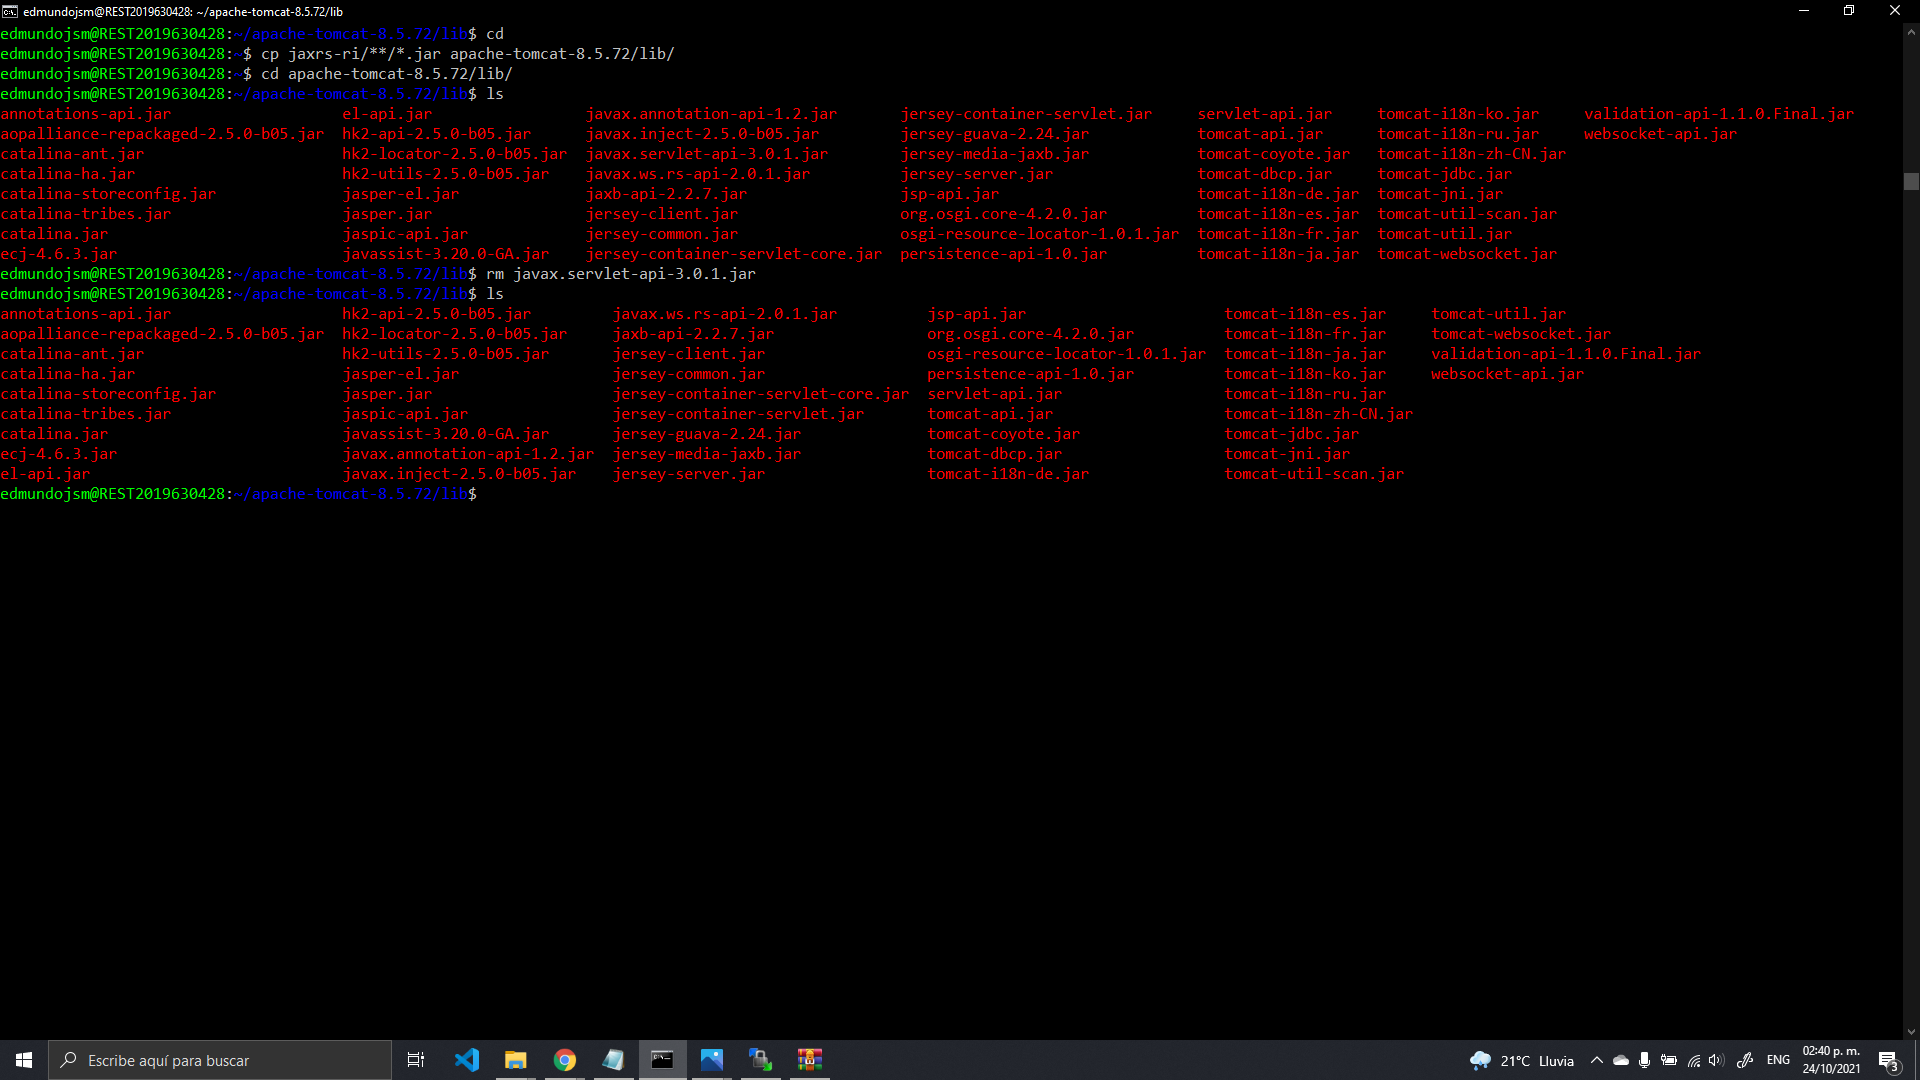
\includegraphics[scale=0.34]{resources/p8.2.png}
			\caption{Borramos el archivo javax.servlet-api-3.0.1.jar del directorio "lib" de Tomcat (esto debe hacerse ya que existe una incompatibilidad entre Tomcat y Jersey 2).}\label{fig:picture}
		\end{figure}
		\begin{figure}[H]
			\centering
			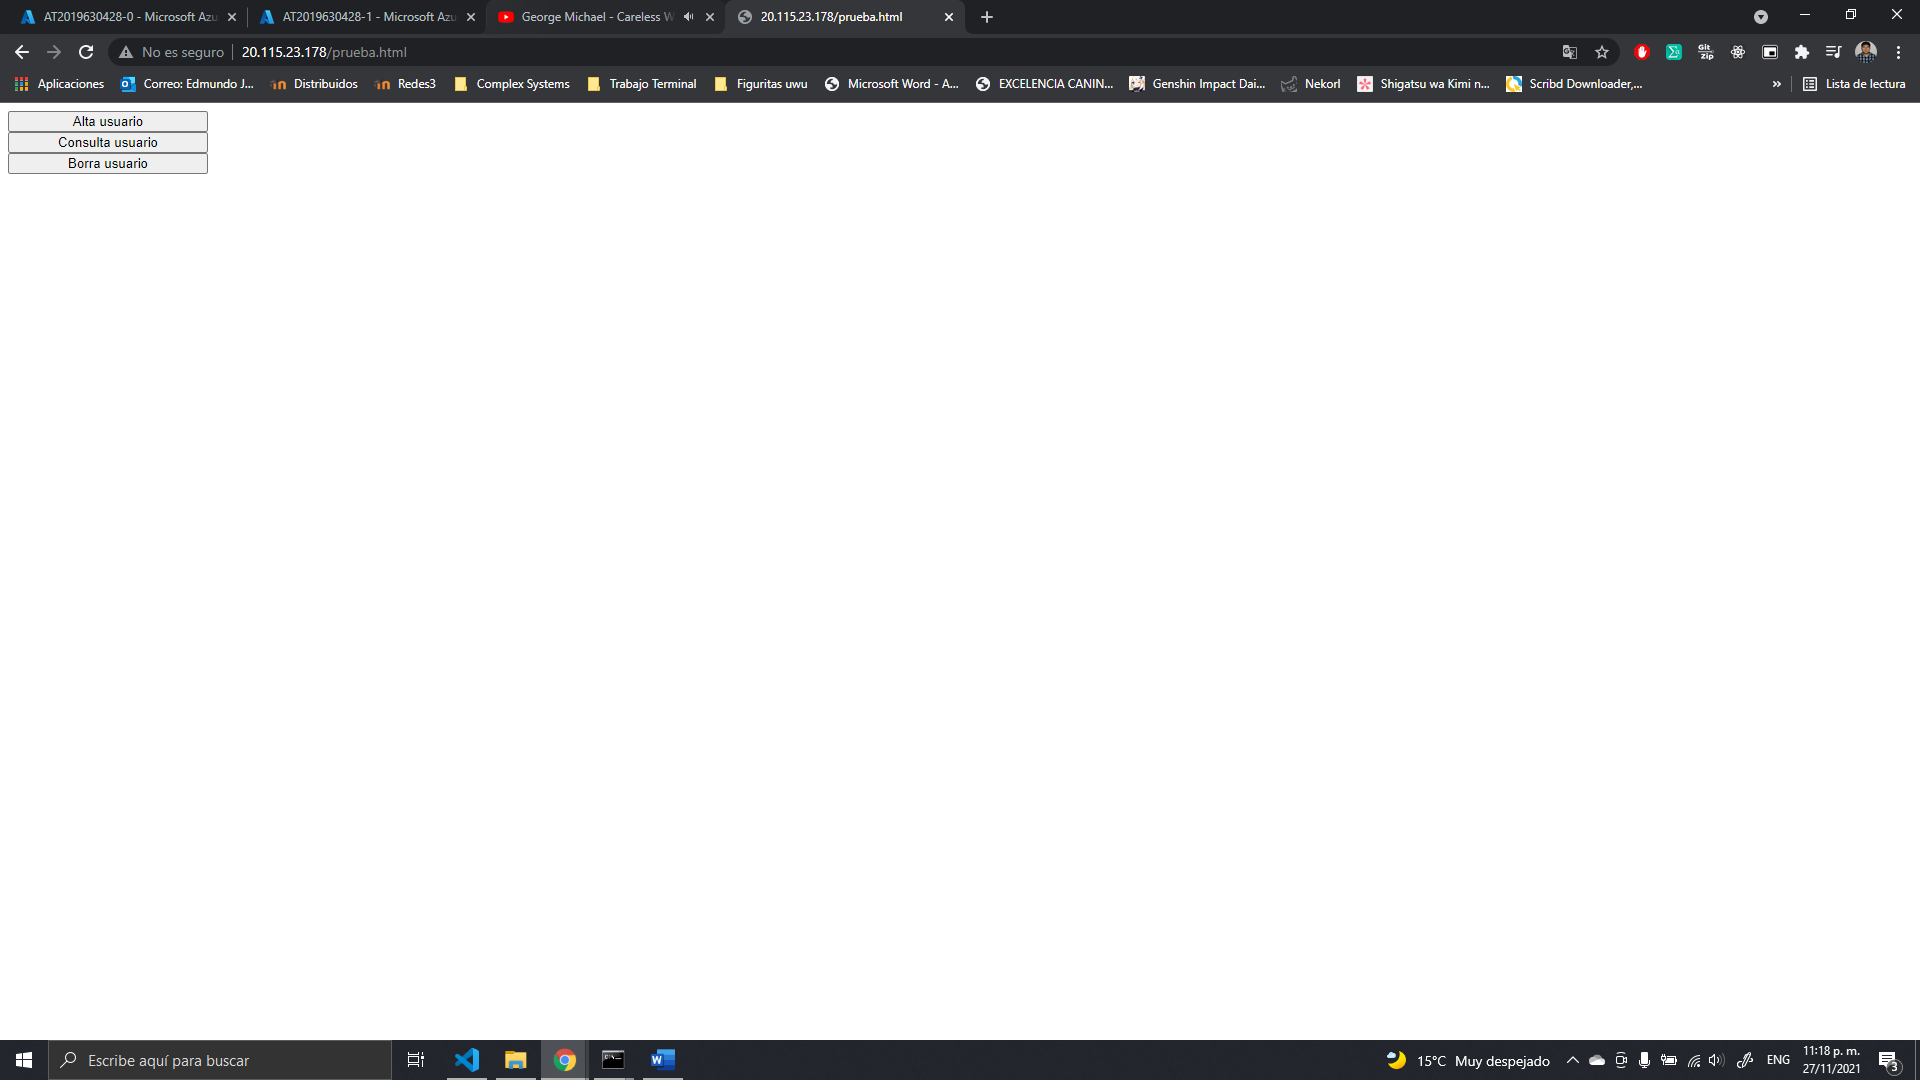
\includegraphics[scale=0.34]{resources/p9.png}
			\caption{Descargamos el archivo gson-2.3.1.jar de la URL https://repo1.maven.org/maven2/com/google
			/code/gson/gson/2.3.1/gson-2.3.1.jar}\label{fig:picture}
		\end{figure}
		\begin{figure}[H]
			\centering
			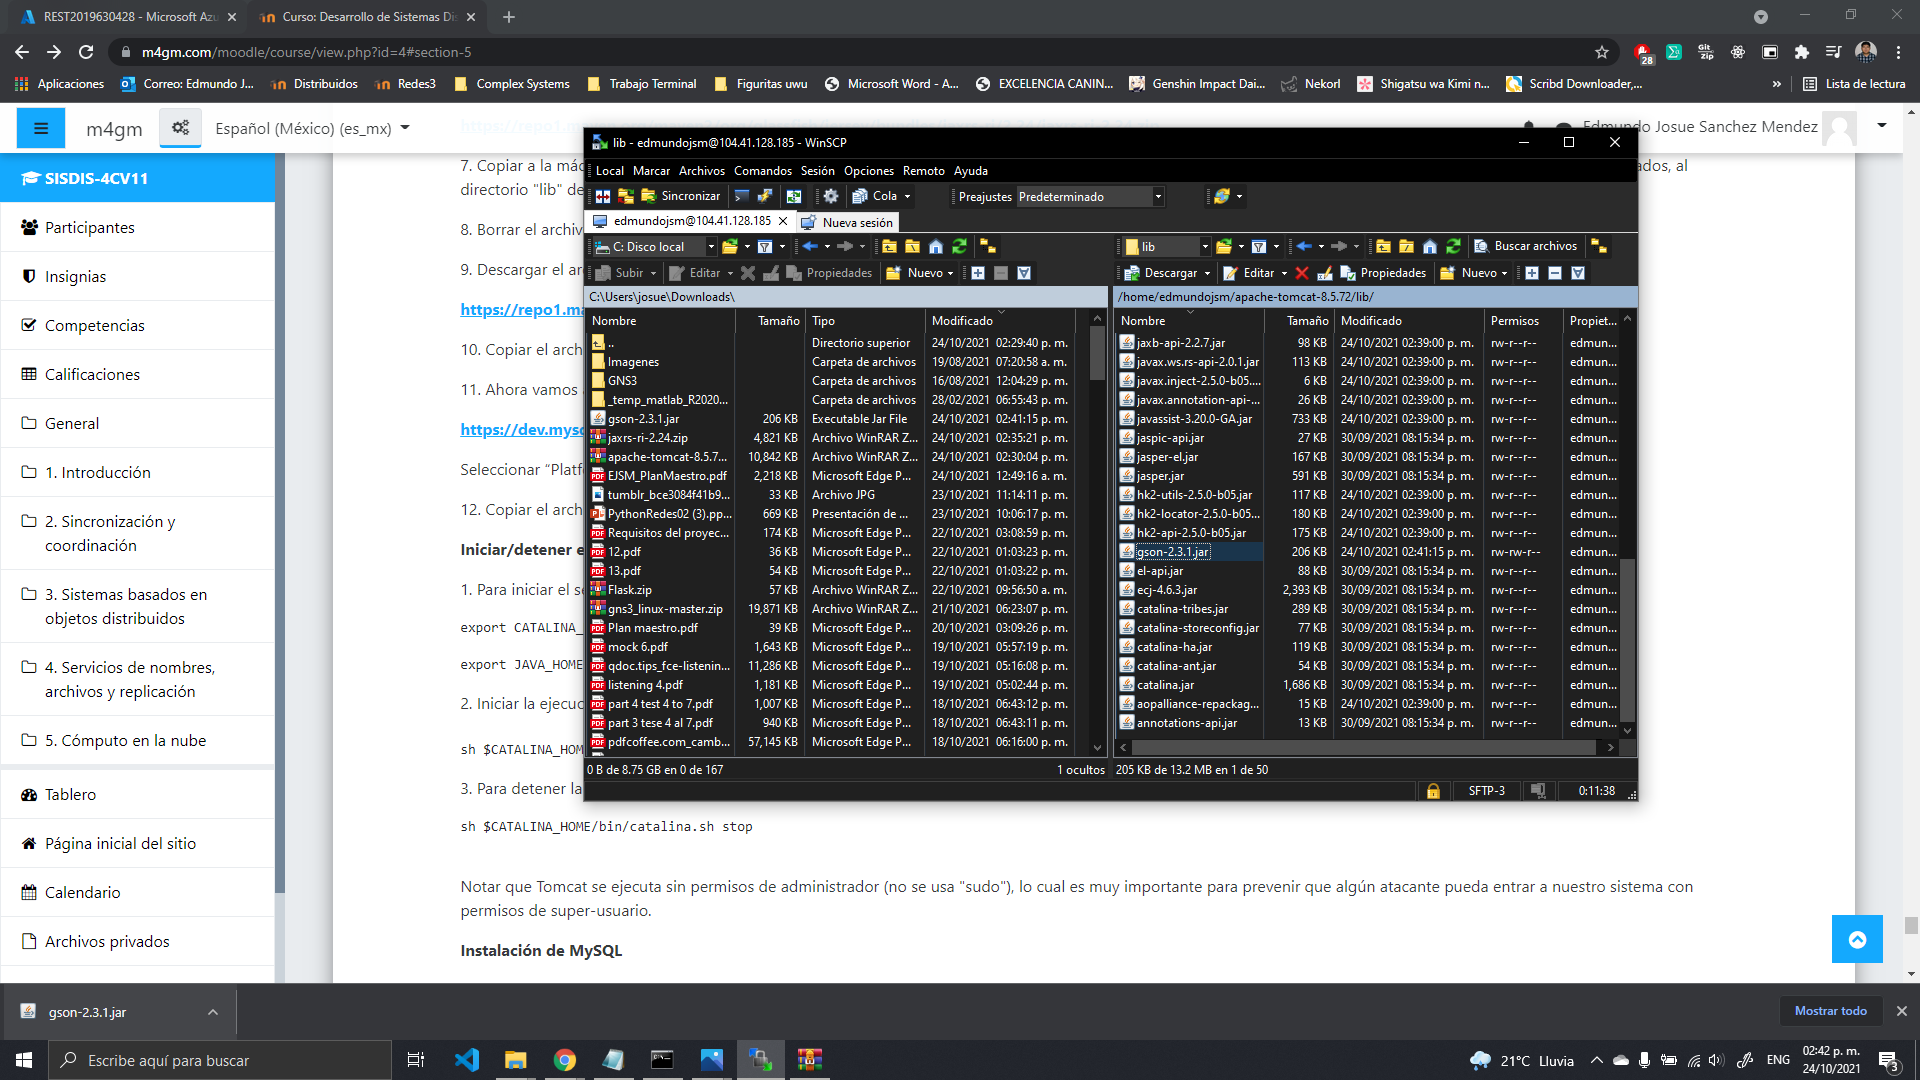
\includegraphics[scale=0.34]{resources/p10.png}
			\caption{Copiamos el archivo gson-2.3.1.jar al directorio "lib" de Tomcat.}\label{fig:picture}
		\end{figure}
		\begin{figure}[H]
			\centering
			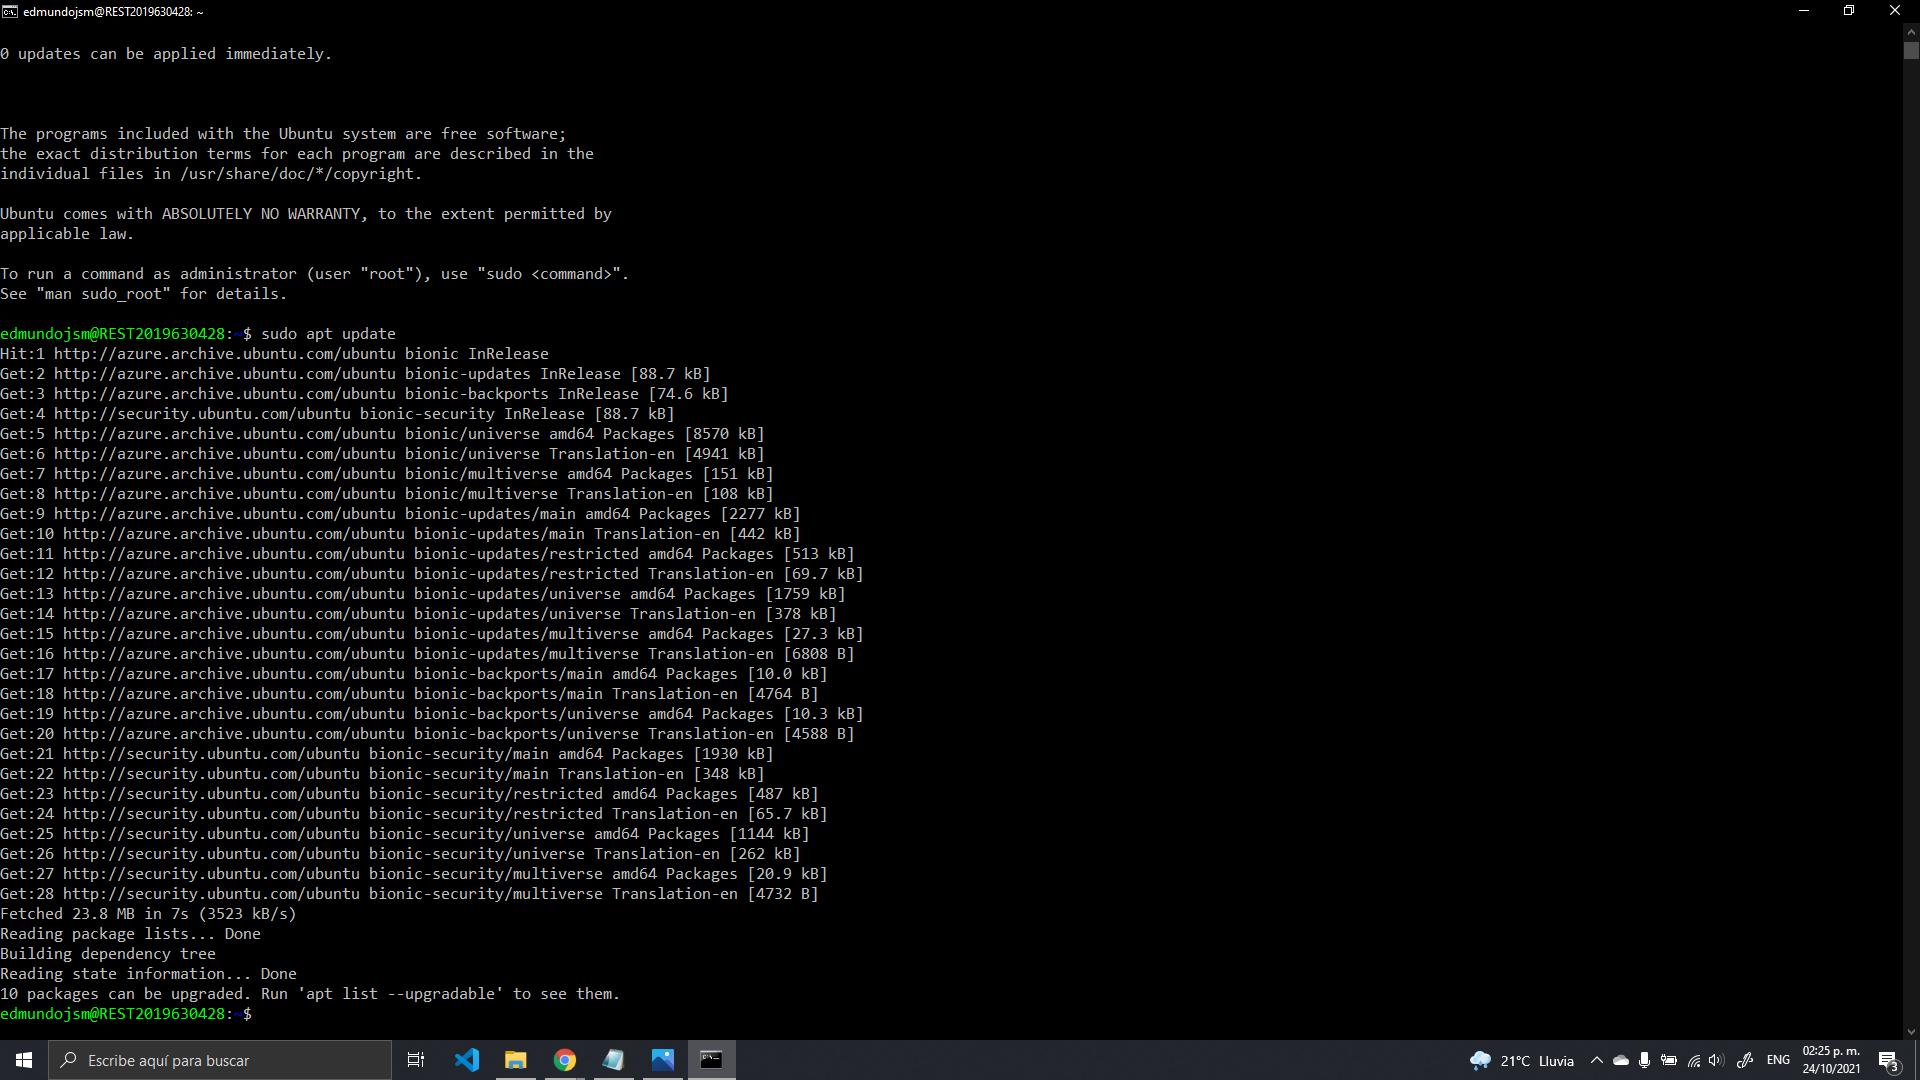
\includegraphics[scale=0.34]{resources/p2.1.png}
			\caption{Ahora instalamos el driver de JDBC para MySQL, lo descargamos desde la URL
https://dev.mysql.com/downloads/connector/j/ seleccionando la opción “Platform independent“ y descargamos el archivo ZIP.}\label{fig:picture}
		\end{figure}
		\begin{figure}[H]
			\centering
			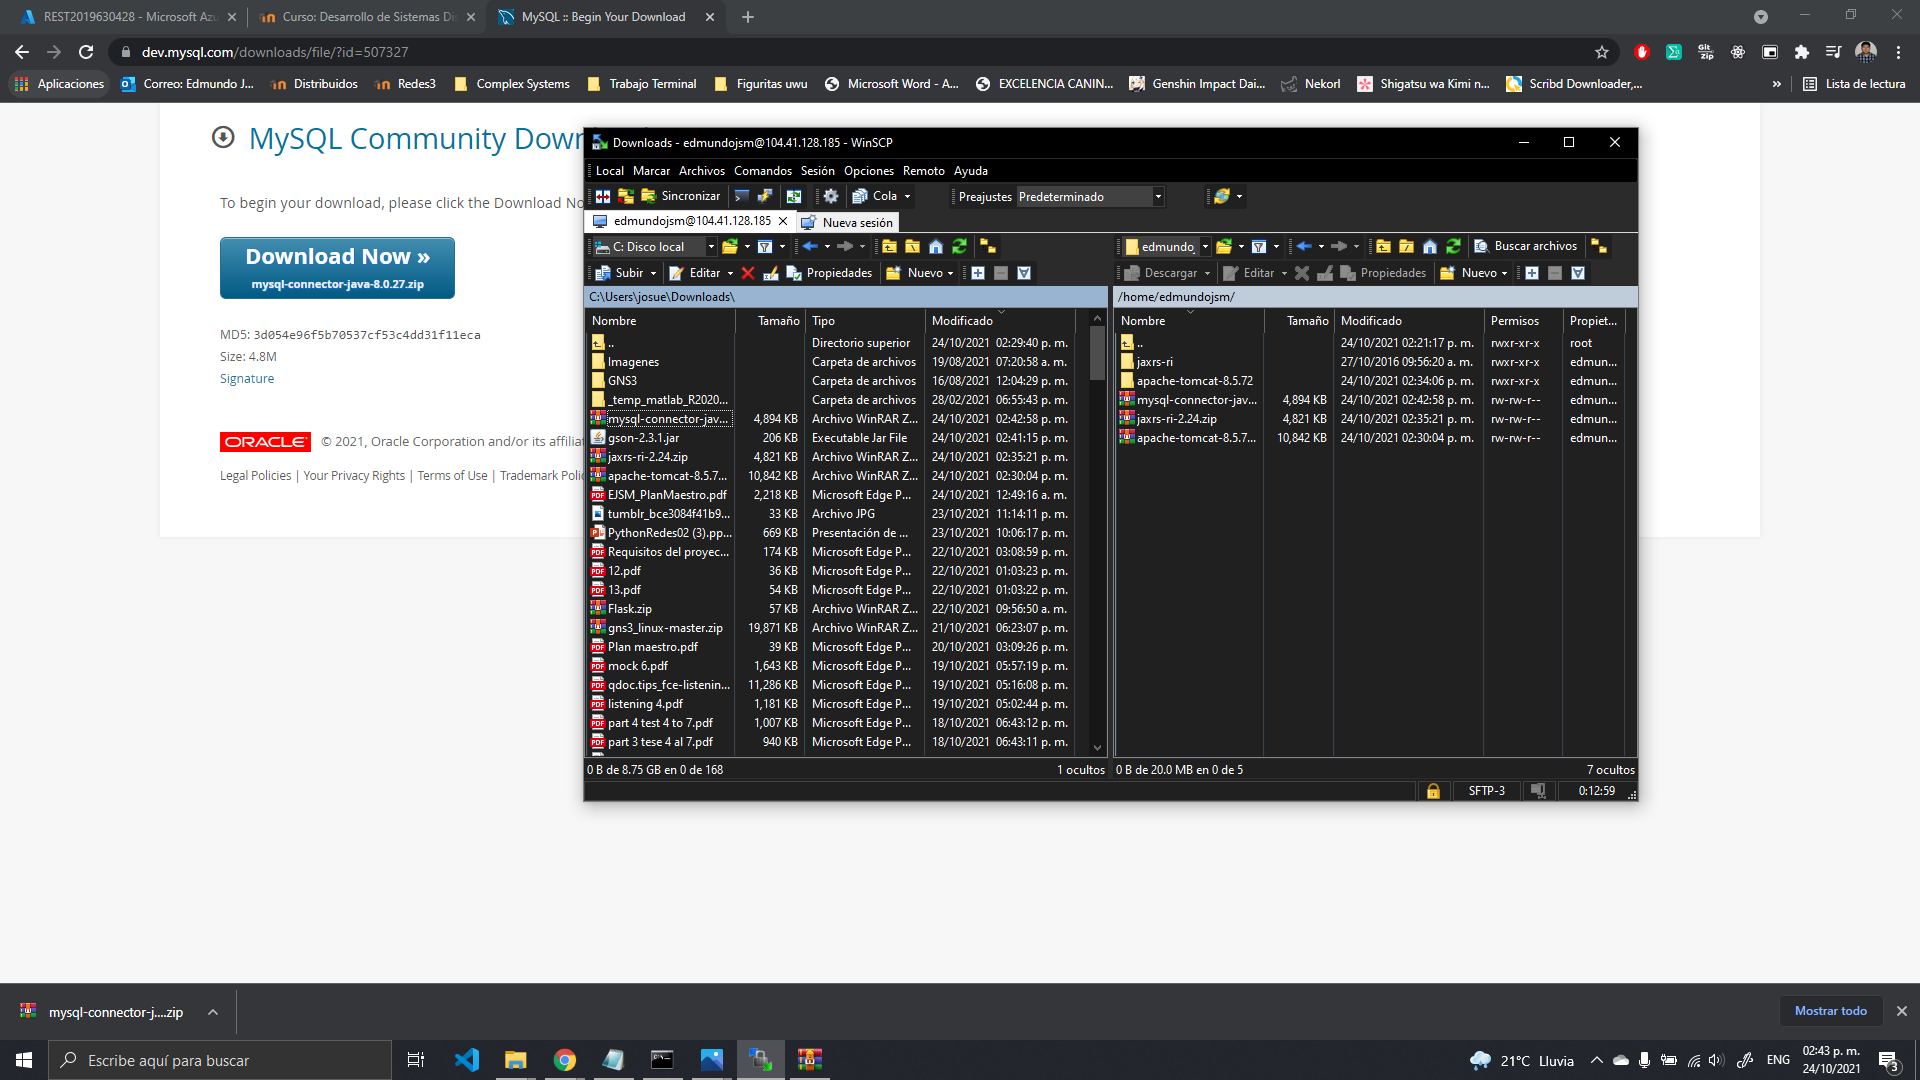
\includegraphics[scale=0.34]{resources/p12.1.png}
			\caption{Copiamos el archivo descargado a la máquina virtual.}\label{fig:picture}
		\end{figure}
		\begin{figure}[H]
			\centering
			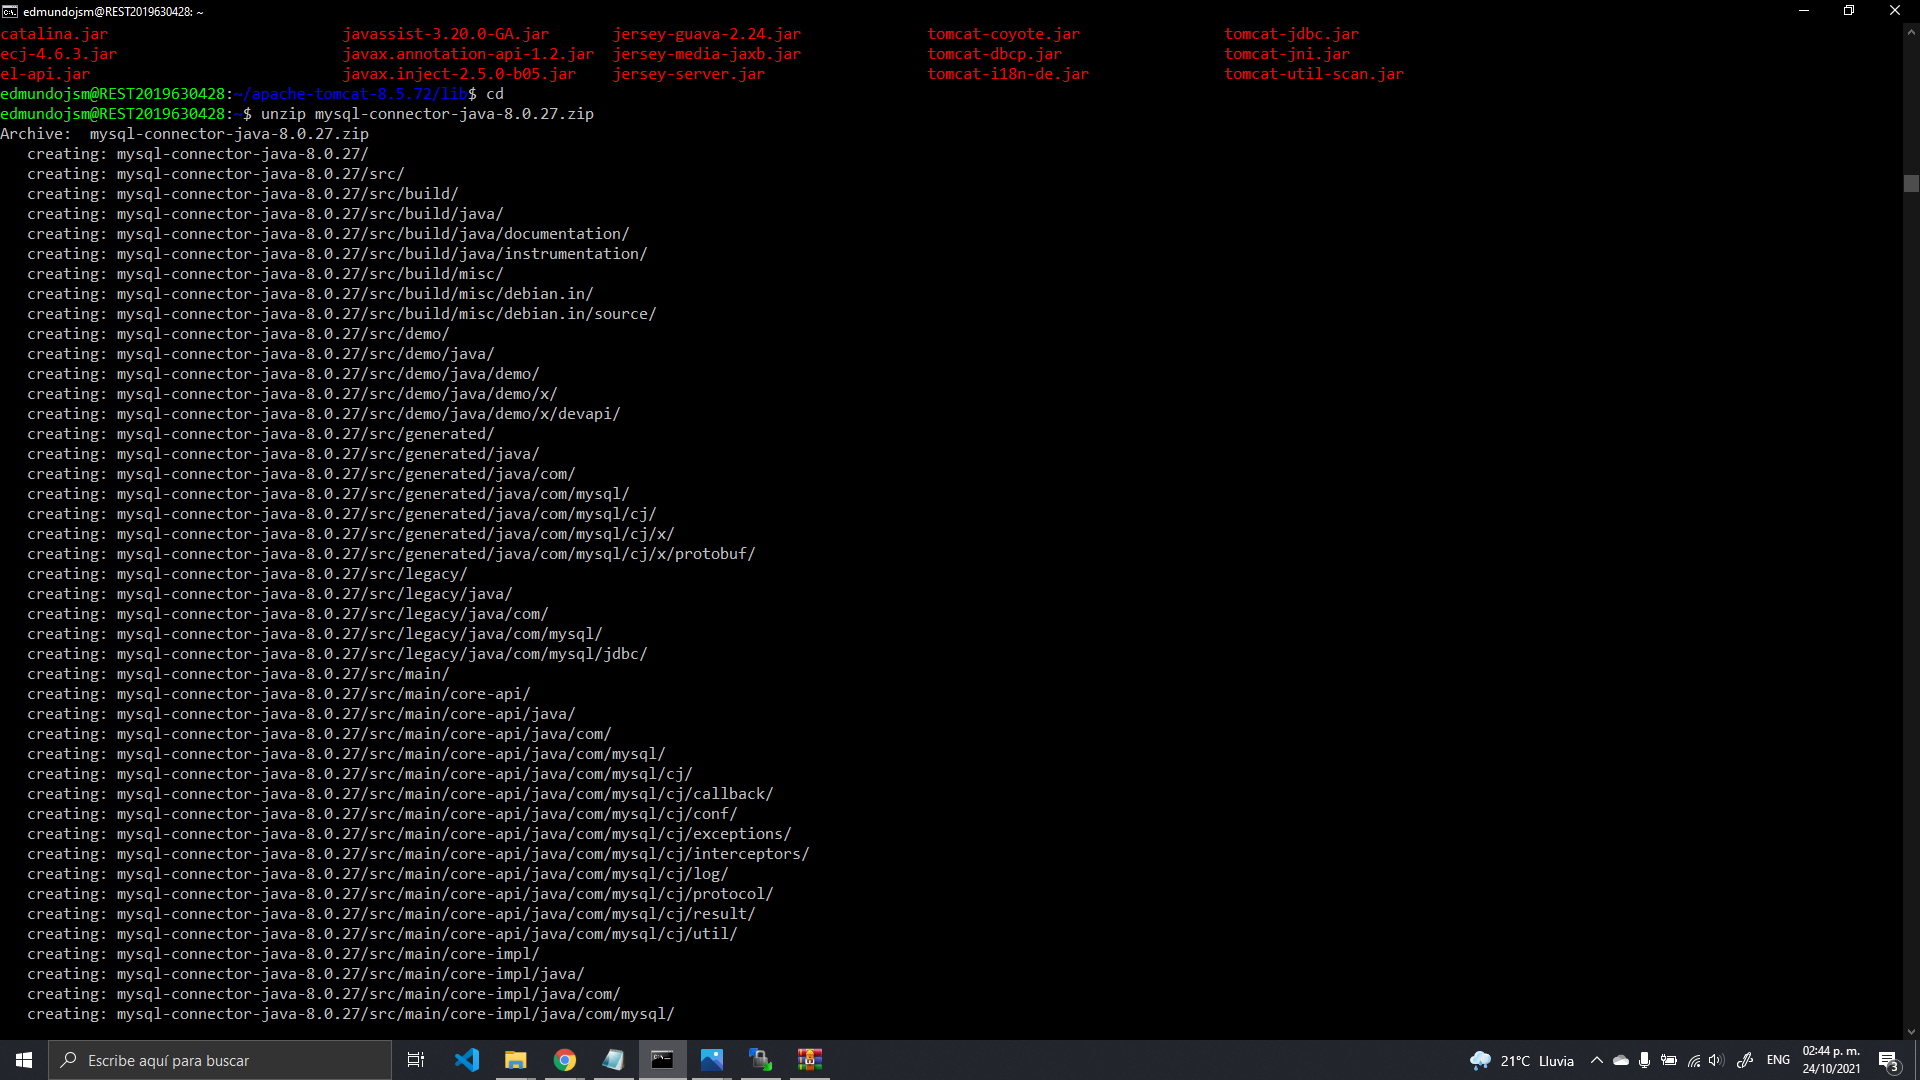
\includegraphics[scale=0.34]{resources/p12.2.png}
			\caption{Desempaquetamos el archivo .zip del paso anterior.}\label{fig:picture}
		\end{figure}
		\begin{figure}[H]
			\centering
			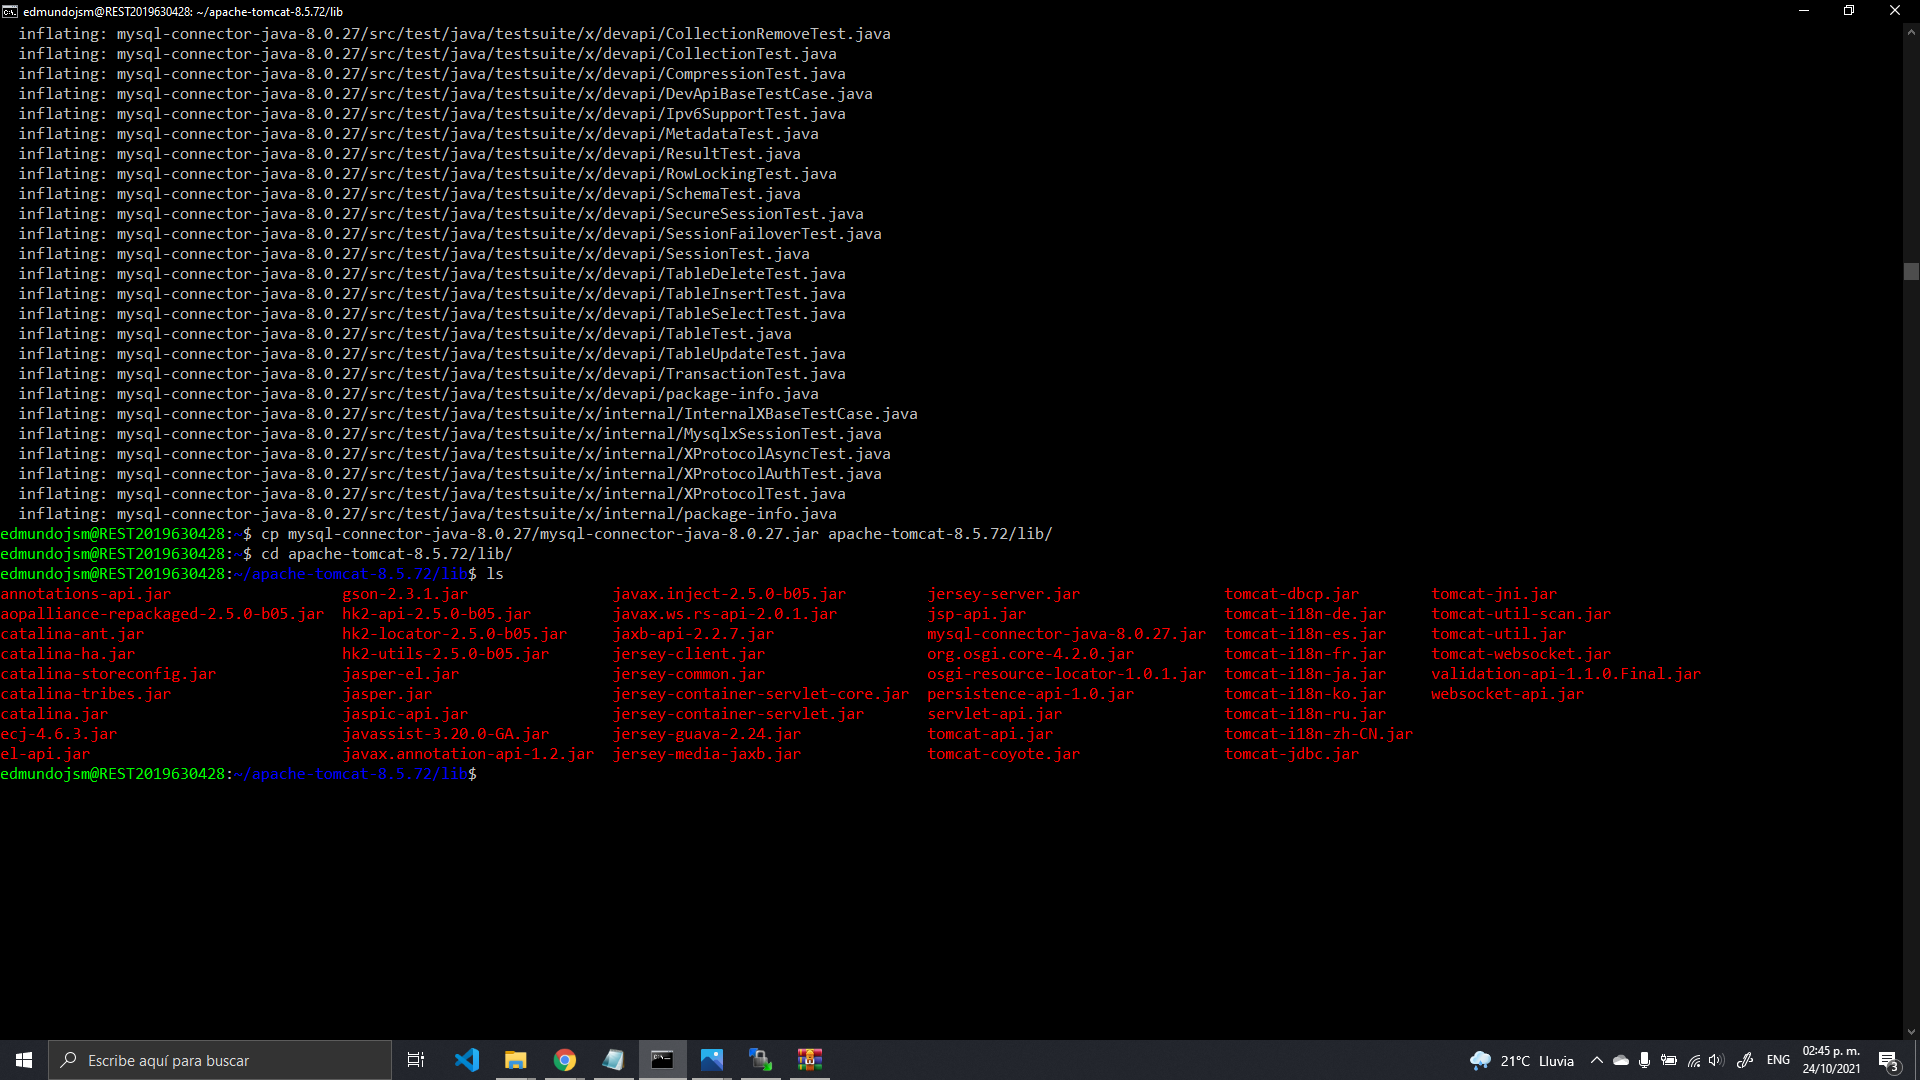
\includegraphics[scale=0.34]{resources/p12.3.png}
			\caption{Copiamos el archivo mysql-connector-java-8.0.27.jar al directorio "lib" de Tomcat.}\label{fig:picture}
		\end{figure}
		\subsection{Iniciar/detener el servidor Tomcat}
		En esta parte configuramos 2 variables de entorno, estas son JAVA\_HOME Y CATALINA\_HOME los cuales se tendrán que asignar las rutas absolutas, para el directorio de java-8-openjdk-amd64 y de Tomcat 8, ademas esto nos sera útil para los siguientes pasos, aparte de iniciar y detener el servidor de Tomcat, para facilitarnos los pasos después de apagar el servidor lo volveremos a iniciar. Todo lo anterior lo vemos en la figura 26.
		\begin{figure}[H]
			\centering
			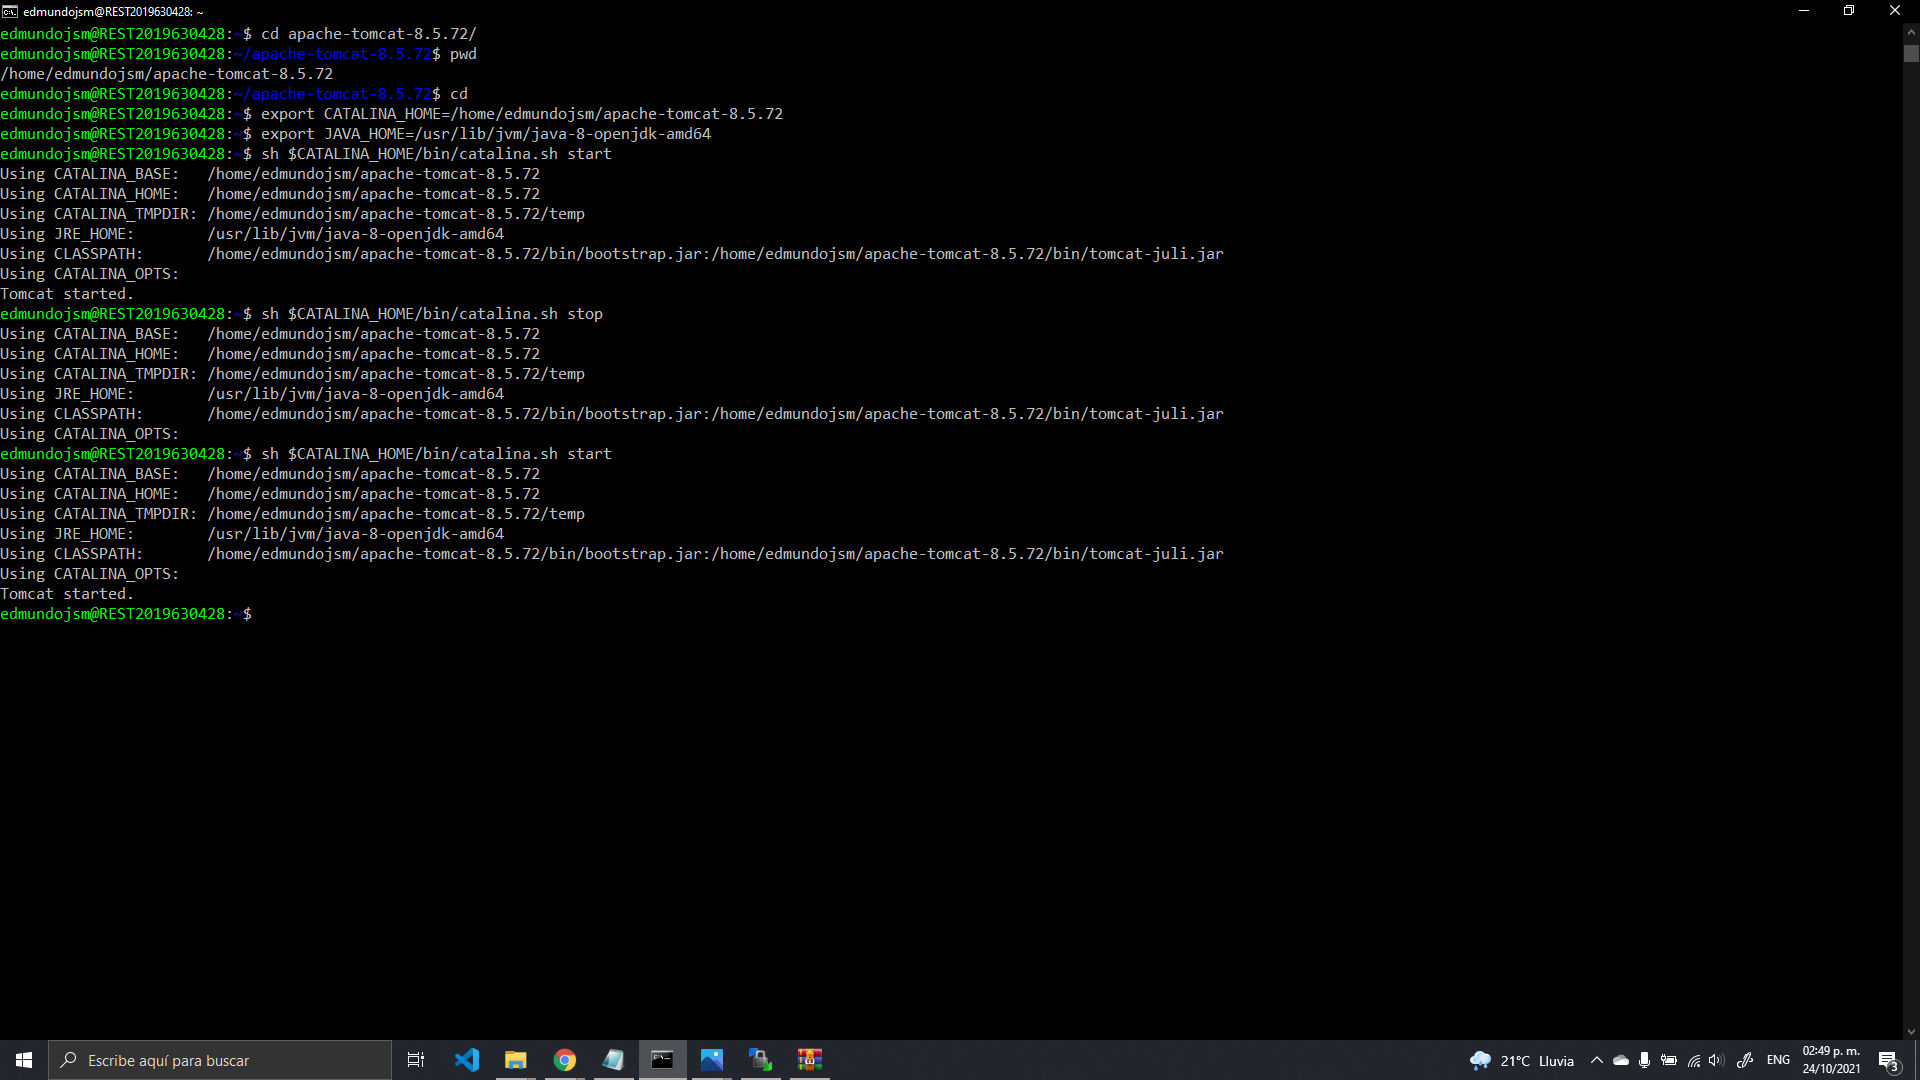
\includegraphics[scale=0.34]{resources/iniciandotomcat.png}
			\caption{Definición de variables de entorno, iniciar, detener y volver a iniciar el servidor de Tomcat.}\label{fig:picture}
		\end{figure}
		\subsection{Instalación de MySQL}
		En la figura 27 vemos como actualizamos los paquetes de la maquina virtual y ademas instalamos el paquete default de MySQL
		\begin{figure}[H]
			\centering
			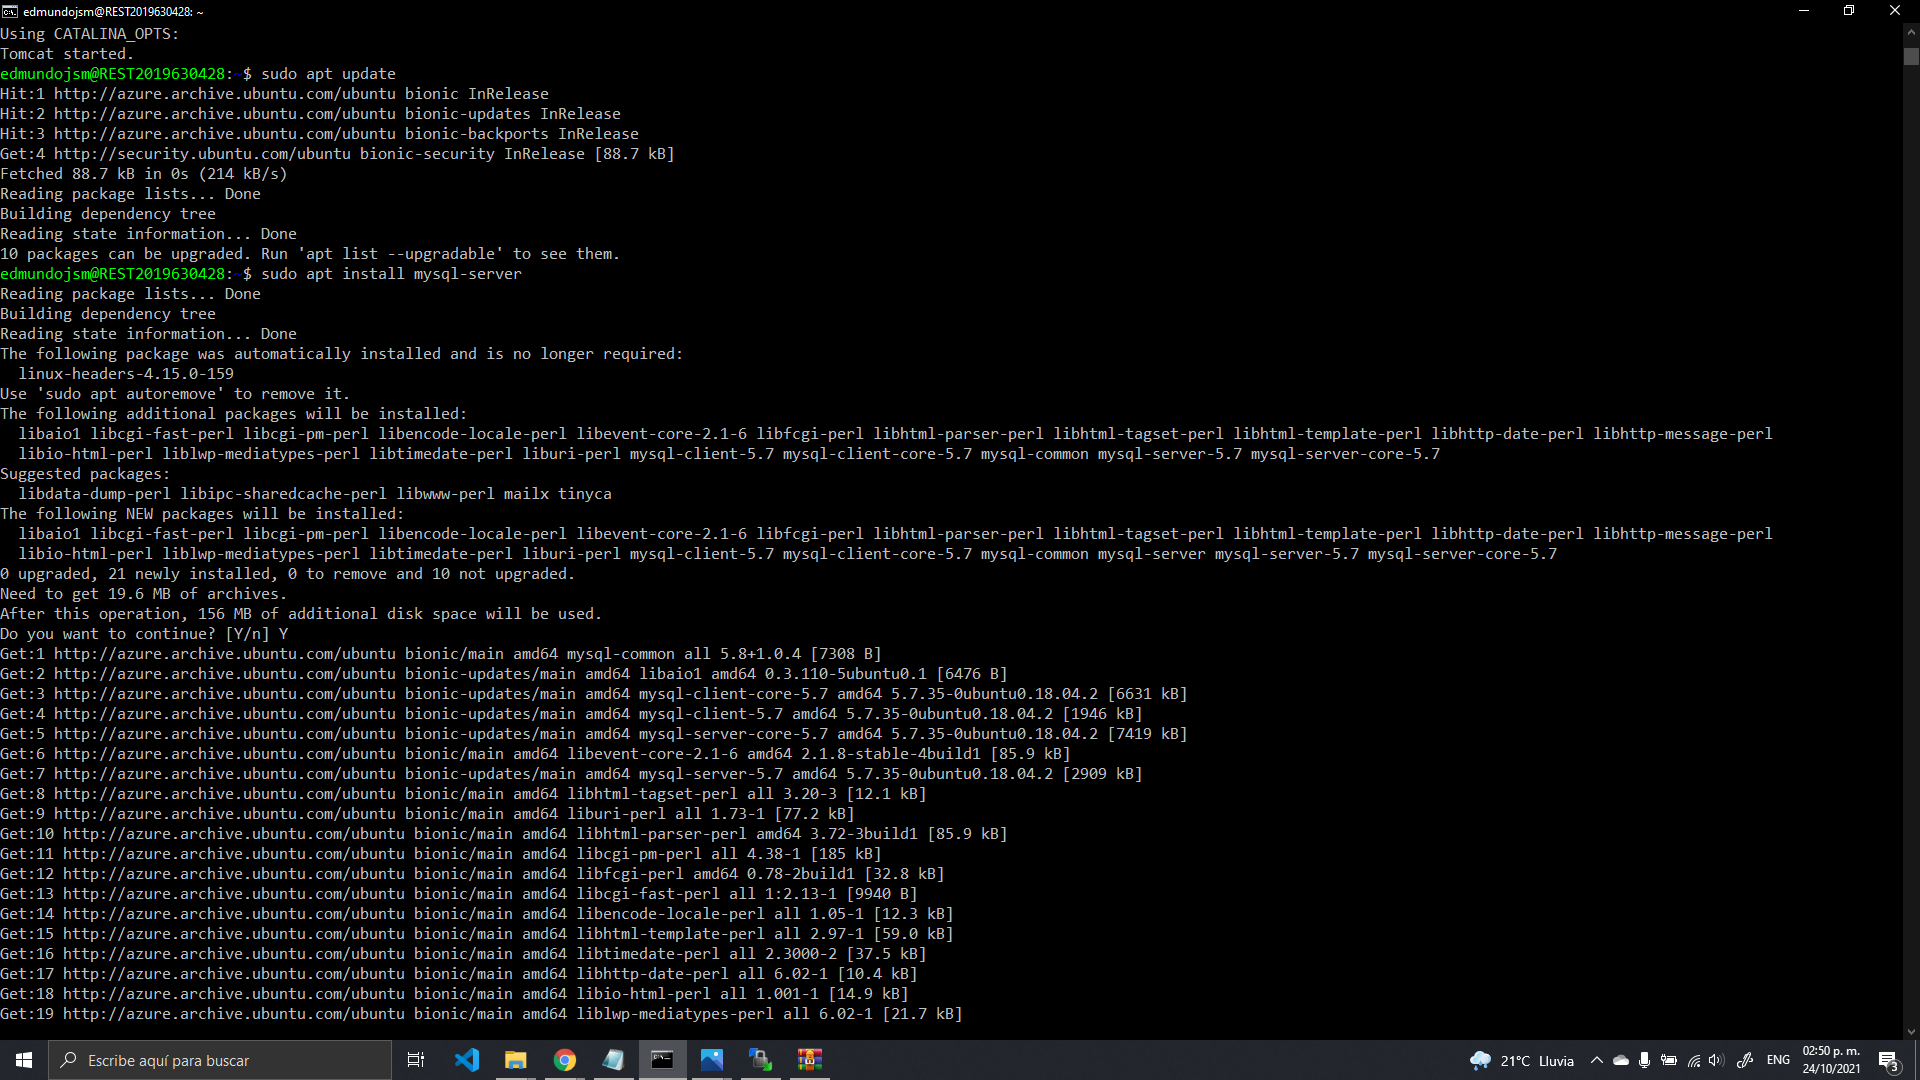
\includegraphics[scale=0.34]{resources/installandomysql.png}
			\caption{Actualizando los paquetes en la maquina virtual e instalando MySQL.}\label{fig:picture}
		\end{figure}
		Ahora en la figura 28 ejecutamos el script de seguridad de MySQL con el fin de poner una contraseña para el usuario root en MySQL.
		\begin{figure}[H]
			\centering
			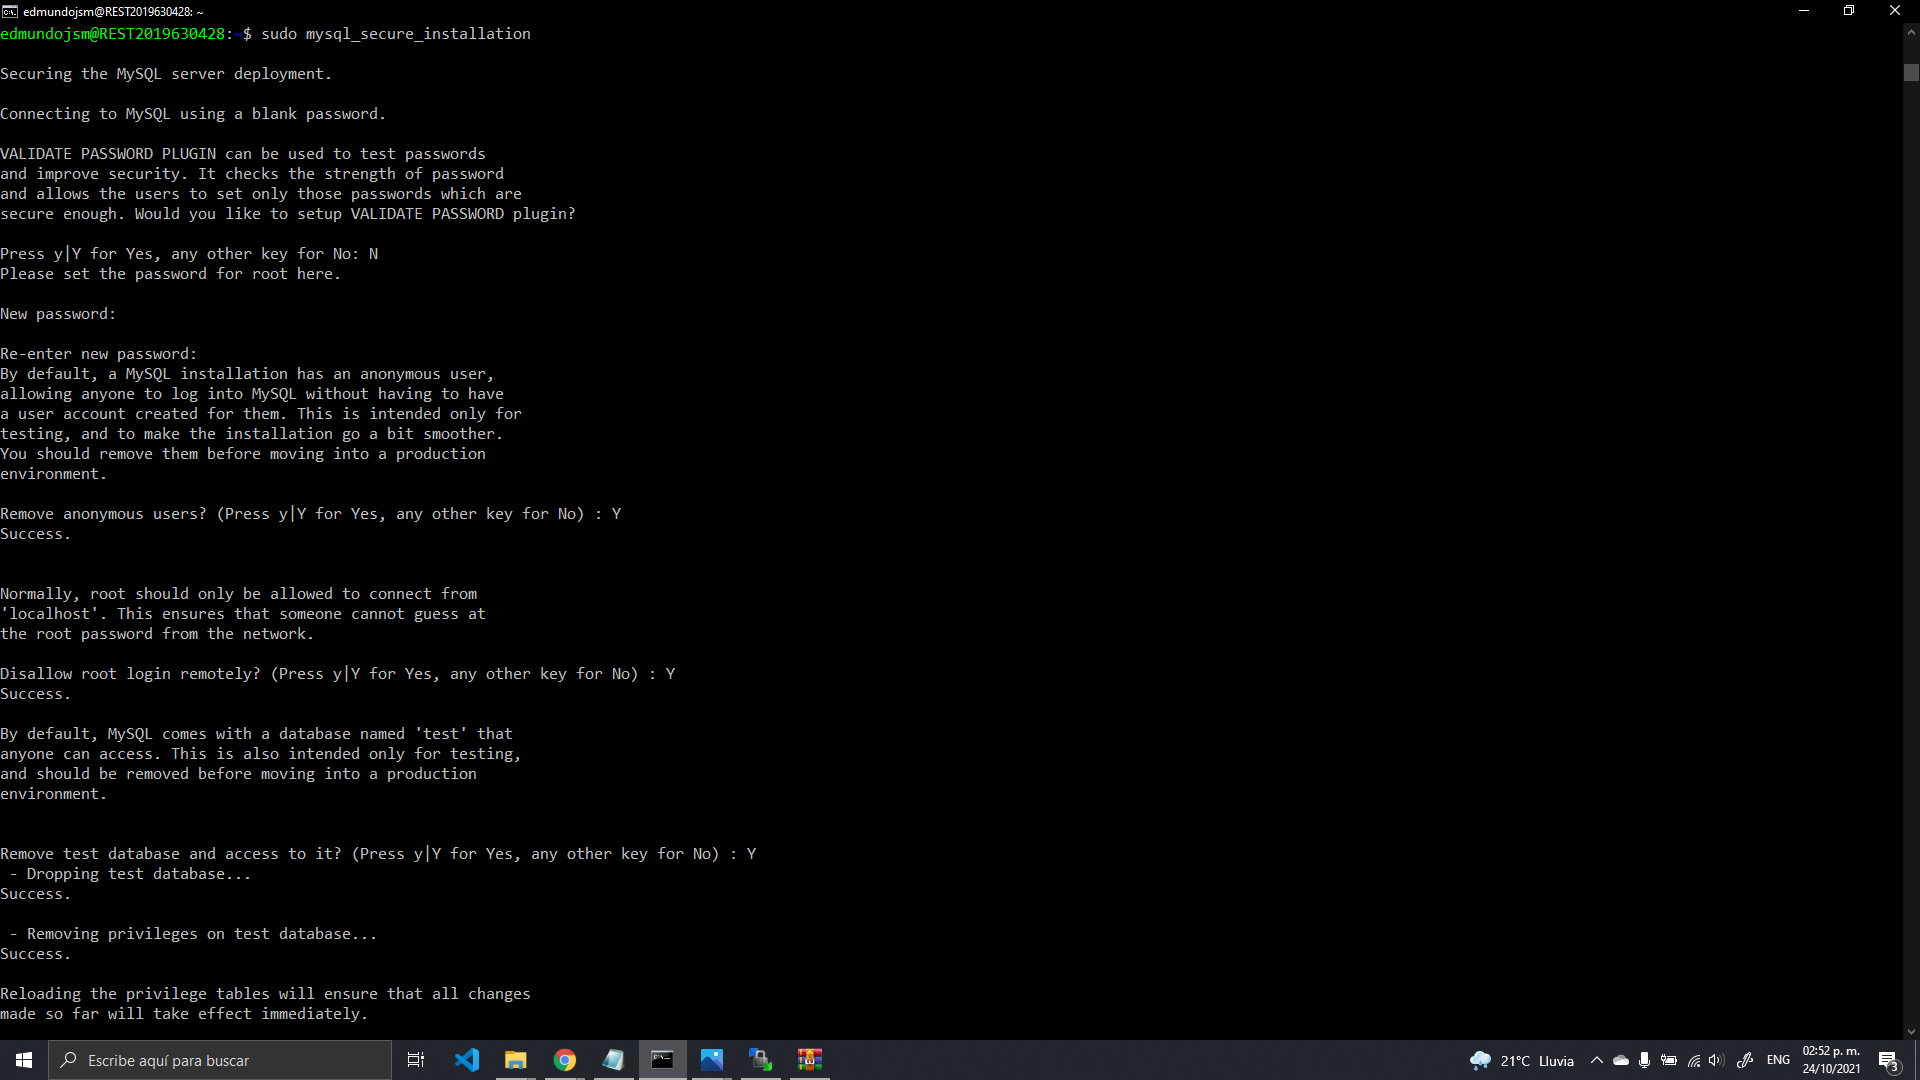
\includegraphics[scale=0.34]{resources/MYSQL3.png}
			\caption{Ejecutando script de seguridad.}\label{fig:picture}
		\end{figure}
		Una vez realizado lo anterior en la imagen 29 vemos como ejecutamos el monitor de MySQL, ejecutamos un comando SQL el cual nos permite modificar la contraseña de root, actualizamos los privilegios y salimos del monitor de SQL.
		\begin{figure}[H]
			\centering
			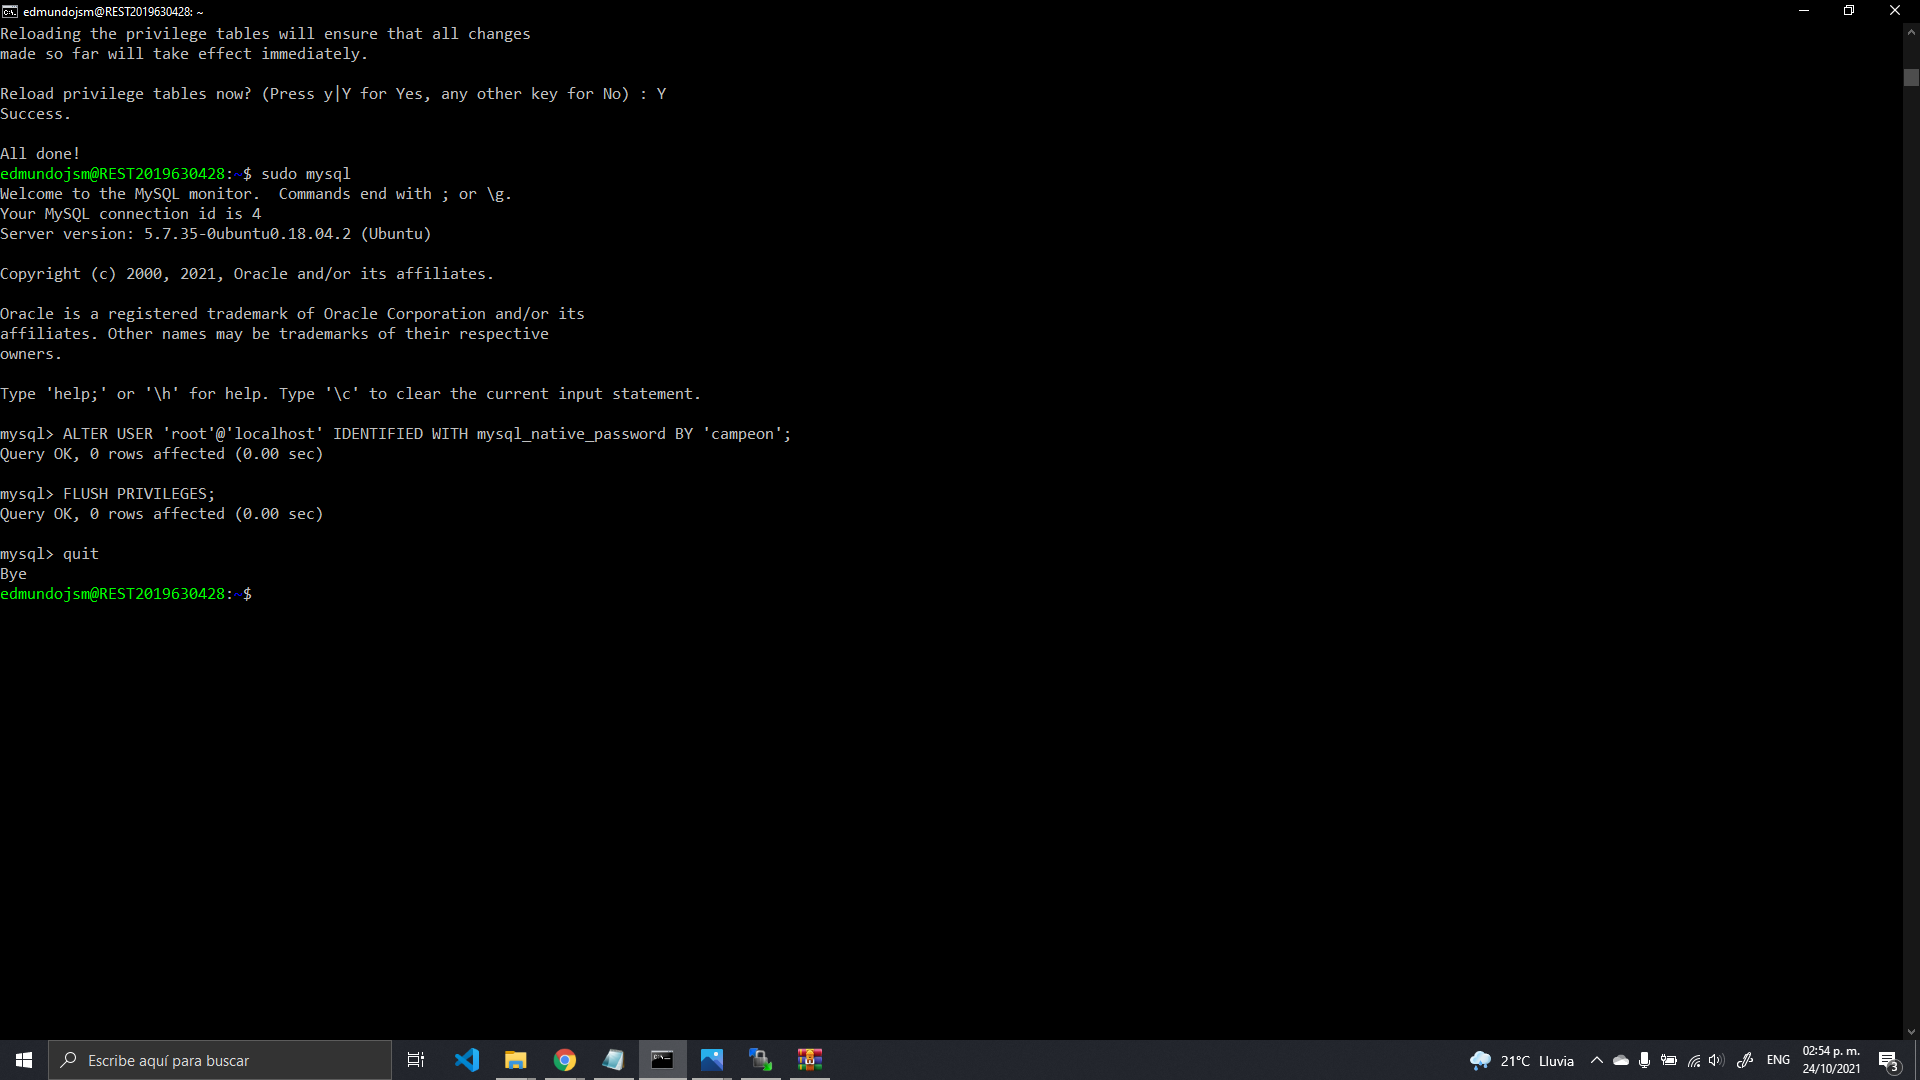
\includegraphics[scale=0.34]{resources/MYSQLF.png}
			\caption{Modificando contraseña de root y actualizando privilegios en el monitor de MySQL.}\label{fig:picture}
		\end{figure}
		\subsection{Creación de un usuario en MySQL}
		En esta parte del proceso crearemos un usuario en MySQL llamado hugo con la contraseña hugo10, ademas de otorgar todos los permisos sobre la base de datos "servicio\_web".
		\begin{figure}[H]
			\centering
			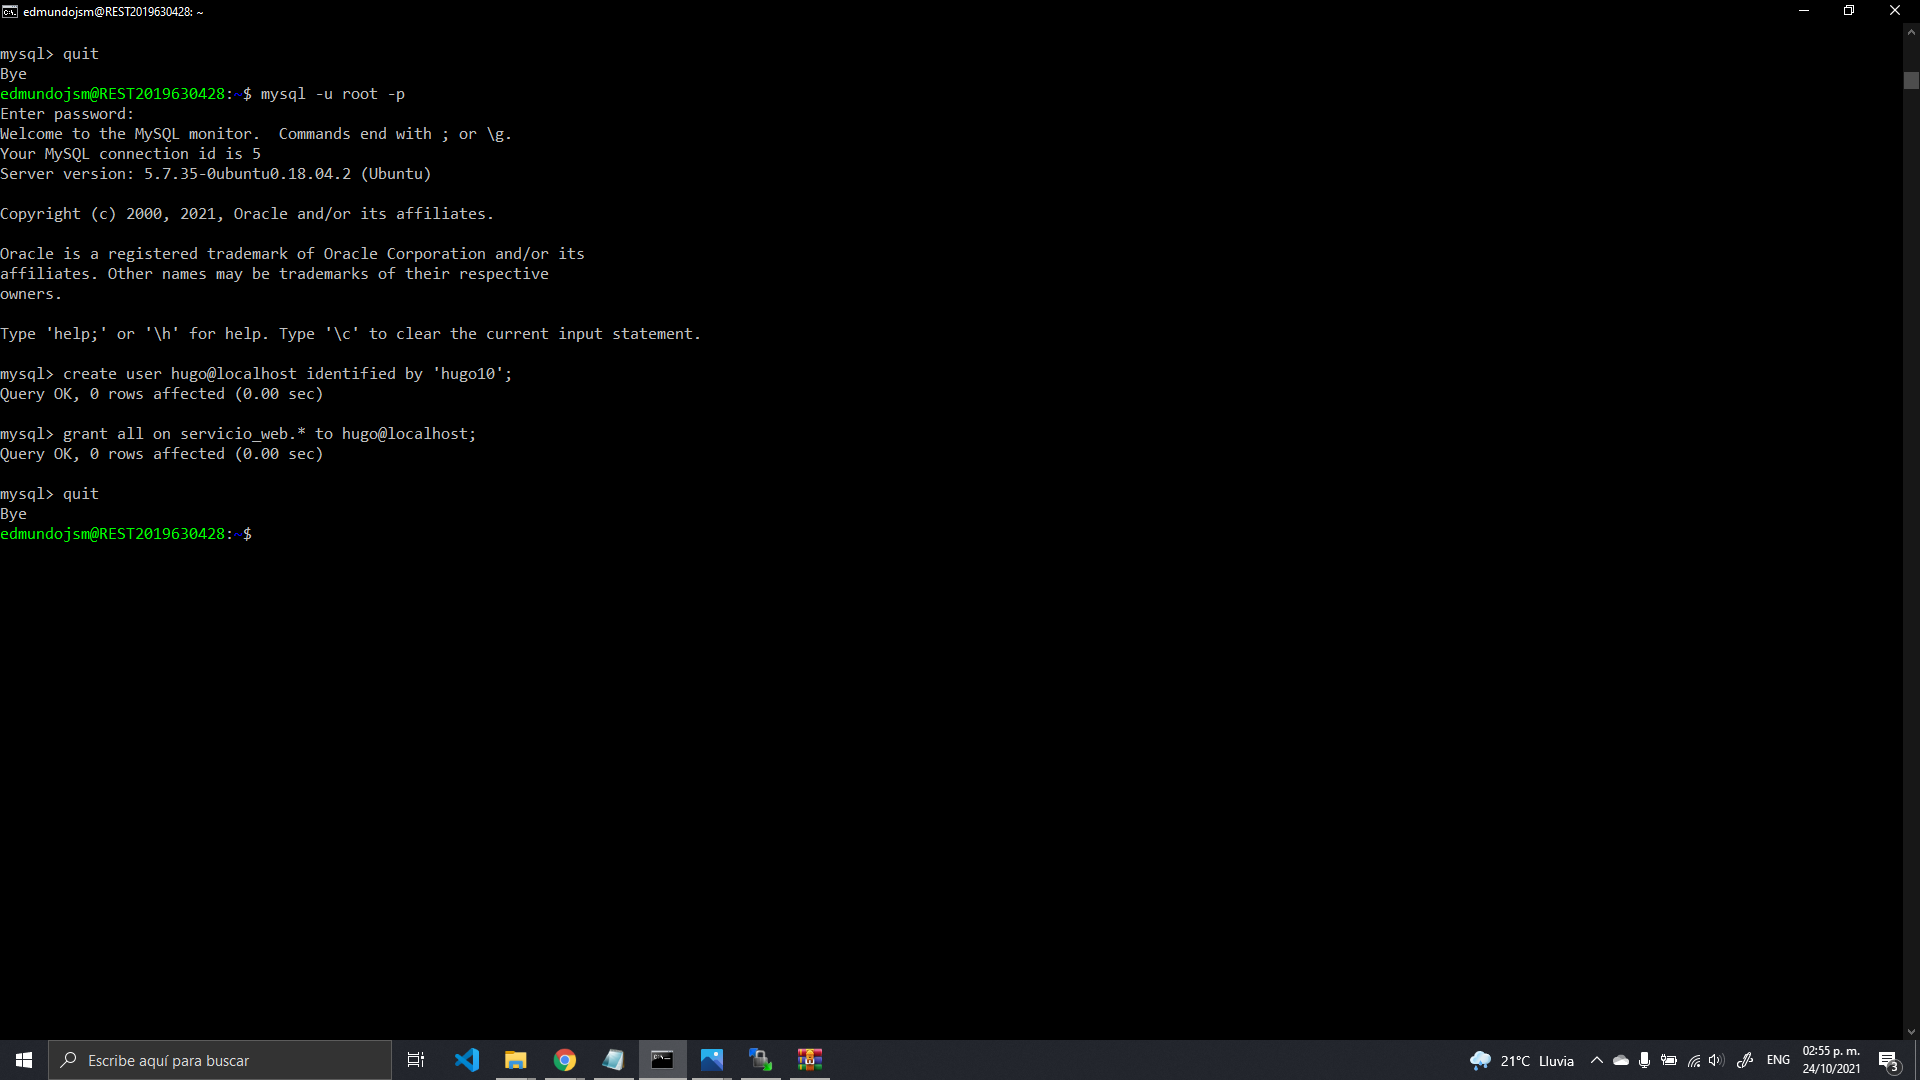
\includegraphics[scale=0.34]{resources/crearusuariook.png}
			\caption{Creación de usuario hugo dando permisos para la base de datos "servicio\_web".}\label{fig:picture}
		\end{figure}
		\subsection{Creación de la base de datos servicio\_web}
		En esta parte del procedimiento crearemos la base de datos a utilizar para esta practica la cual sera administrada por el usuario hugo, para esta ocasión tendremos que usar dos tablas, la de usuarios y la de fotos de los usuarios, las cuales tendrán las siguientes tablas con los tipos de datos correspondientes.
		\begin{verbatim}
			create table usuarios
			(
			    id_usuario integer auto_increment primary key,
			    email varchar(256) not null,
			    nombre varchar(100) not null,
			    apellido_paterno varchar(100) not null,
			    apellido_materno varchar(100),
			    fecha_nacimiento date not null,
			    telefono varchar(20),
			    genero char(1)
			);
			create table fotos_usuarios
			(
			    id_foto integer auto_increment primary key,
			    foto longblob,
			    id_usuario integer not null
			);
		\end{verbatim}
		Una vez creados tendremos que ingresar los siguientes comandos los cuales hacen la referencia entre las tablas y crean una llave primaria la cual sera el email en la tabla de usuarios.
		\begin{verbatim}
			alter table fotos_usuarios add foreign key (id_usuario) references usuarios(id_usuario);
			create unique index usuarios_1 on usuarios(email);
		\end{verbatim}
		Todo lo anterior se hará en el monitor MySQL pasando el usuario hugo, todo lo anterior lo podemos ver en la figura 31 , recordando que al finalizar tenemos que salir del monitor MySQL.
		\begin{figure}[H]
			\centering
			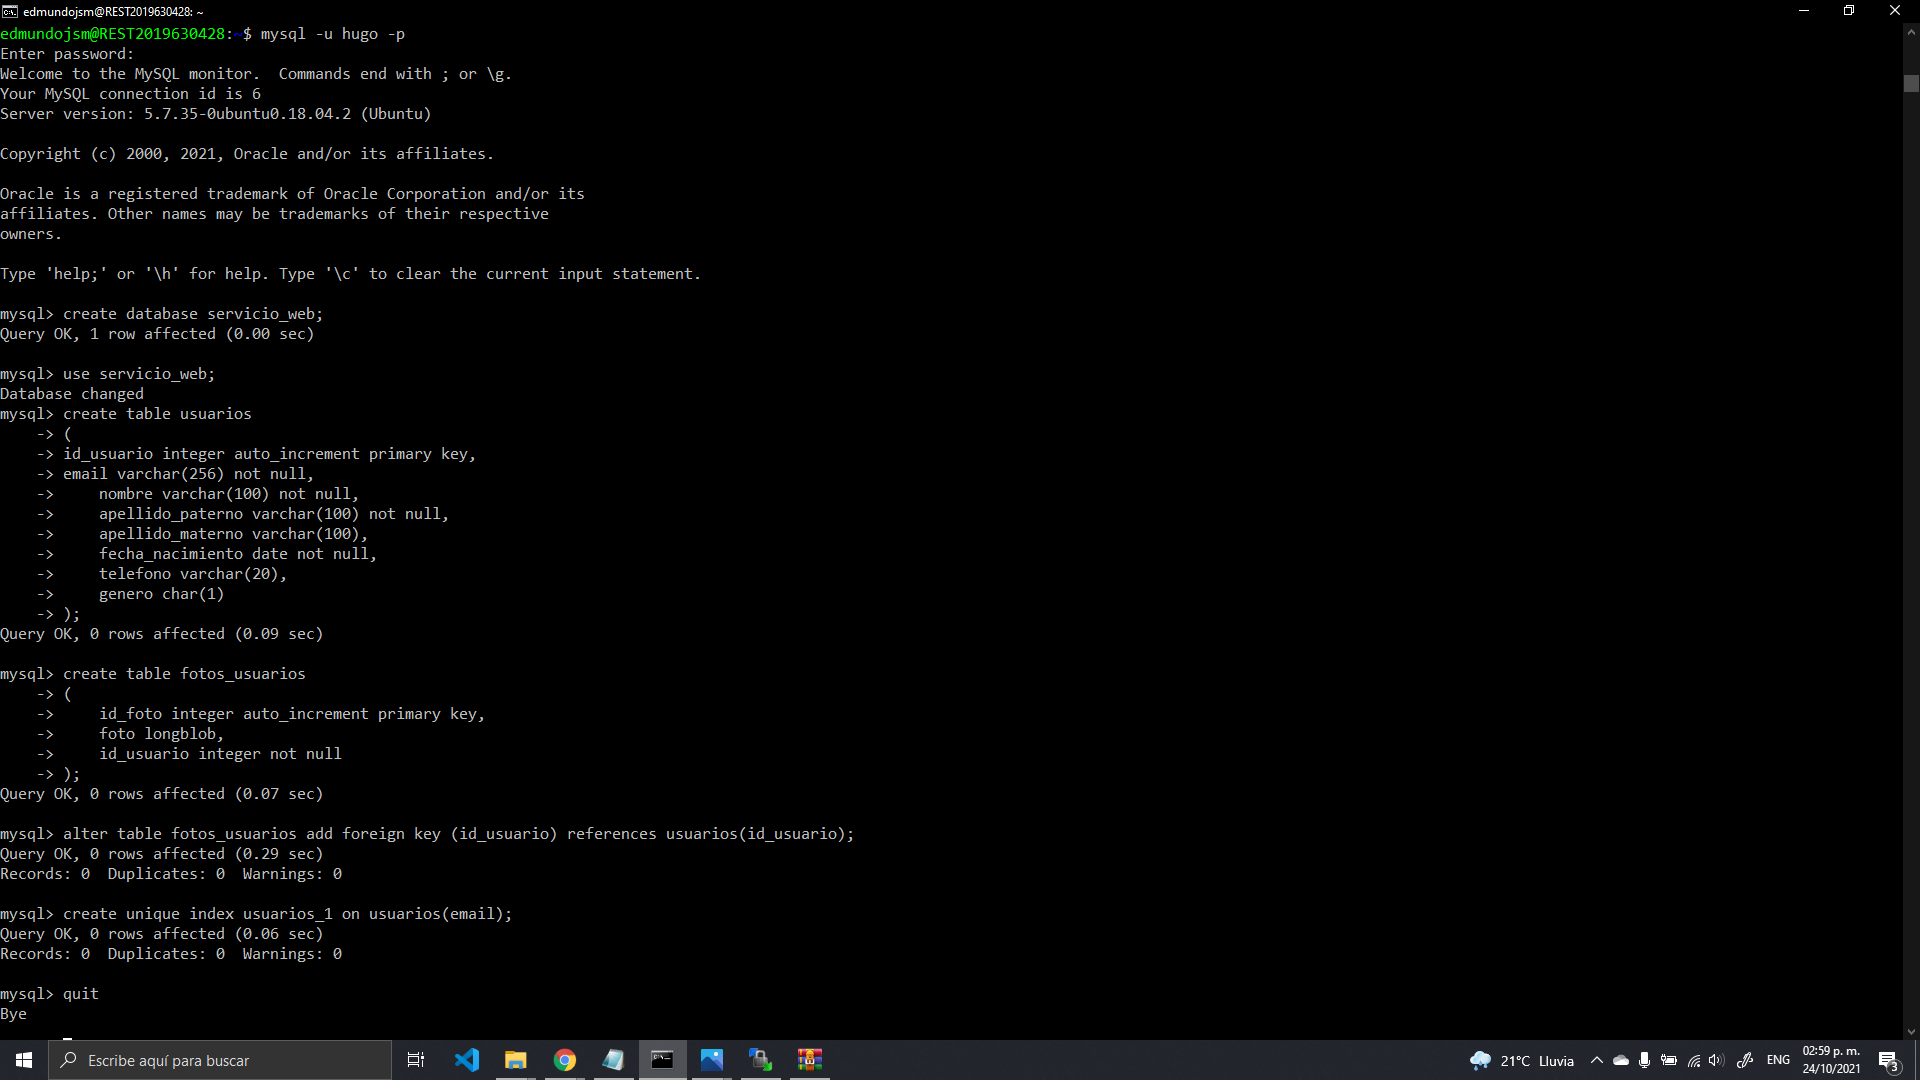
\includegraphics[scale=0.34]{resources/bdok.png}
			\caption{Creacion de la base de datos "servicio\_web".}\label{fig:picture}
		\end{figure}
		\subsection{Compilar, empacar y desplegar el servicio web}
		Para esta sección se compila, empaca y se despliega el servicio web, esto hará que el servicio web este prácticamente listo para su uso, sin embargo, nos faltara agregar 3 archivos los cuales son WSCliente.js, prueba.html y usuario\_sin\_foto.png los cuales son archivos necesarios para el correcto funcionamiento del programa, prácticamente es la parte del front-end. Para poder lograrlo tendremos que seguir lo que se muestra en las figuras 32 a la 36.
		\begin{figure}[H]
			\centering
			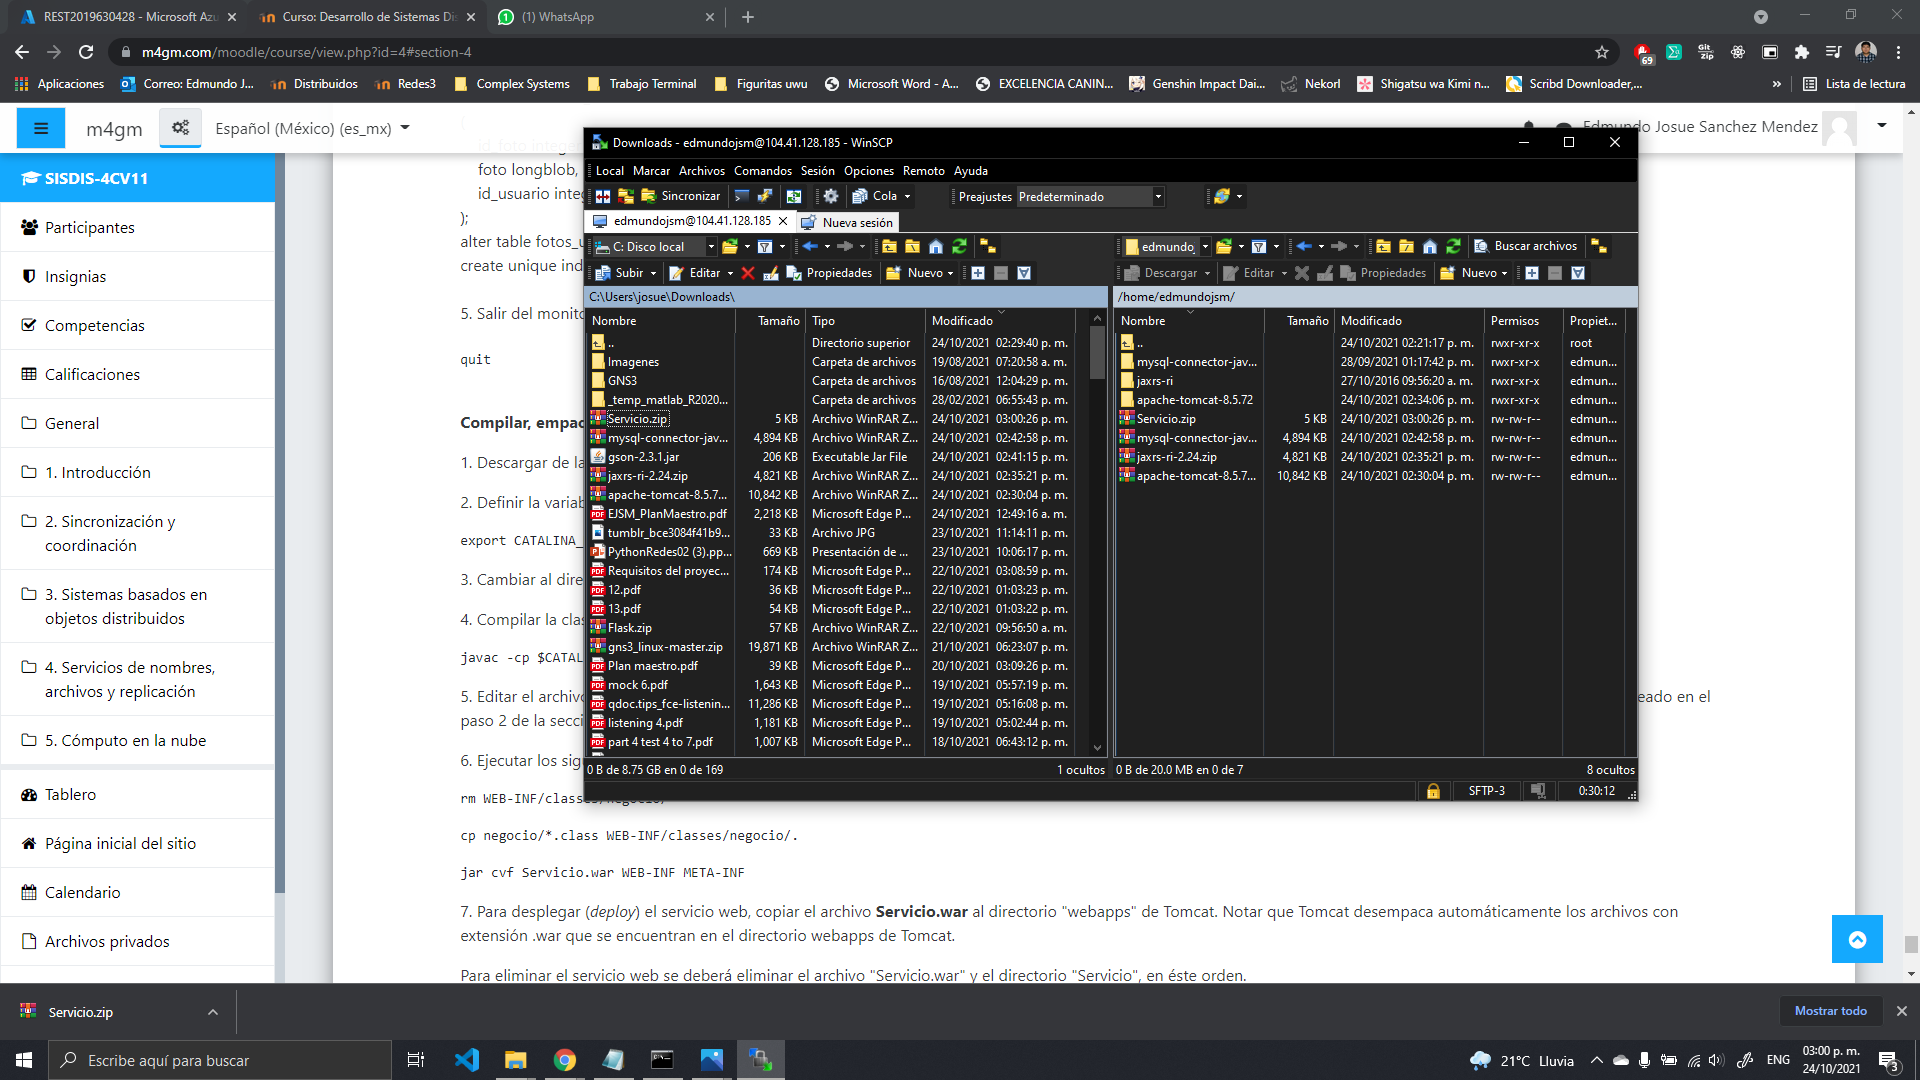
\includegraphics[scale=0.34]{resources/cdb1.png}
			\caption{Archivo Servicio.zip descargado desde de la plataforma y pasado a la maquina virtual.}\label{fig:picture}
		\end{figure}
		\begin{figure}[H]
			\centering
			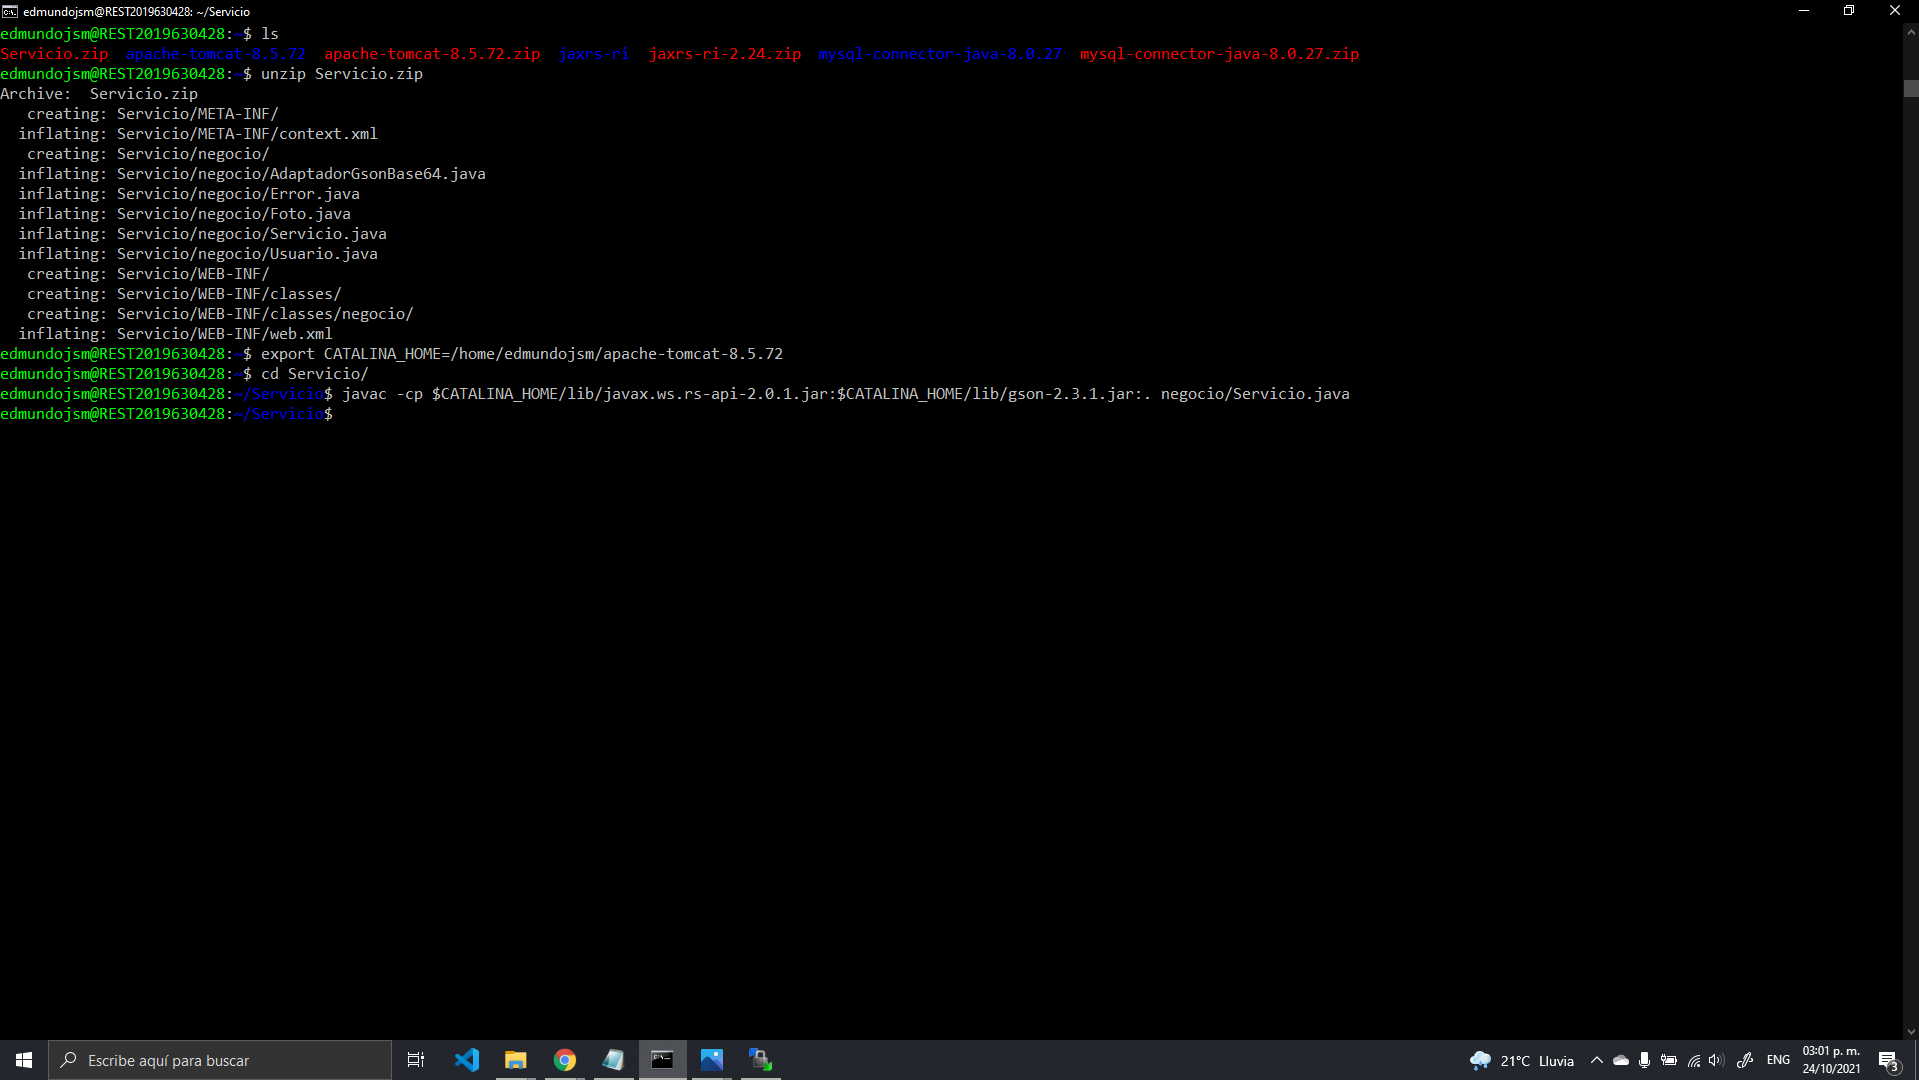
\includegraphics[scale=0.34]{resources/ced1234.png}
			\caption{Desempaque del archivo Servicio.zip, así como definición de la variable de ambiente CATALINA\_HOME, también el cambio de directorio a Servicio para poder compilar la clase Servicio.java.}\label{fig:picture}
		\end{figure}
		\begin{figure}[H]
			\centering
			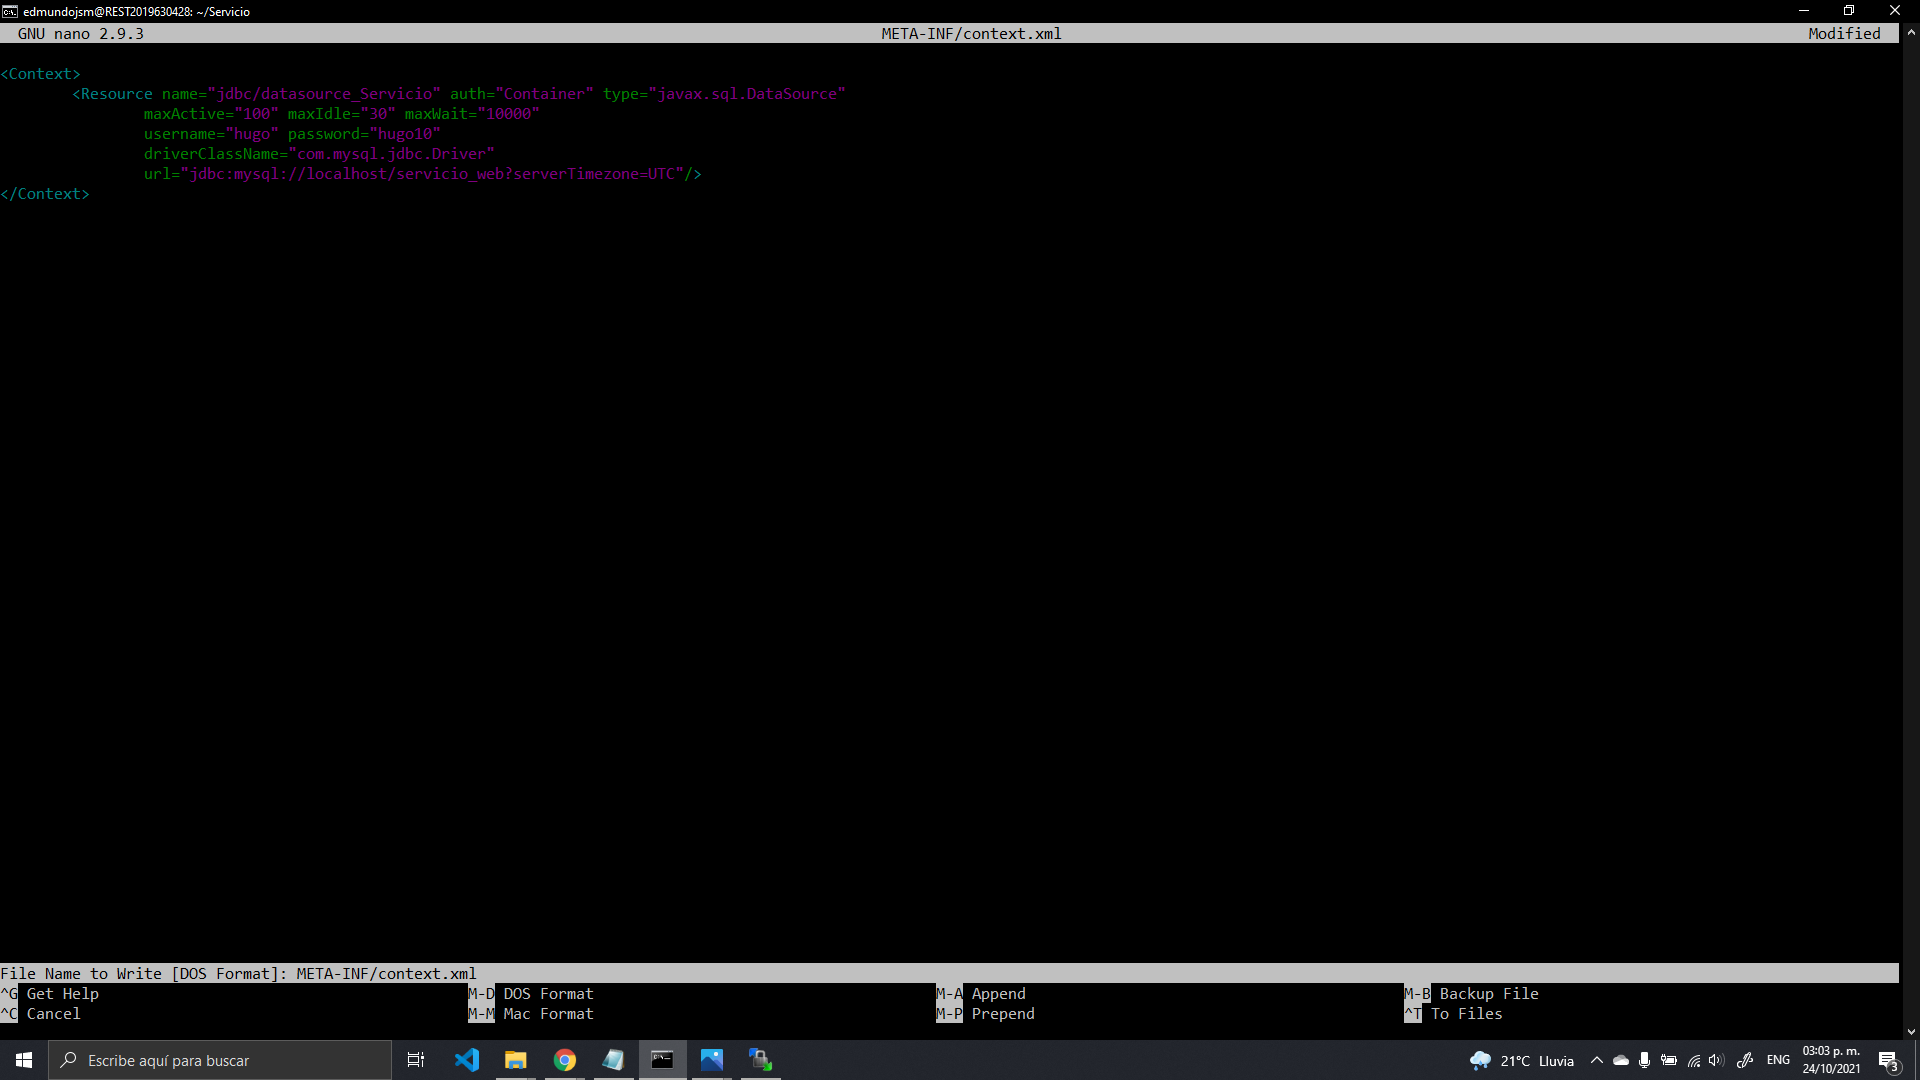
\includegraphics[scale=0.34]{resources/ced5.png}
			\caption{Modificación del archivo context.xml que esta en el directorio META-INF, definiendo el username de la base de datos y el password correspondiente, en este caso es hugo y hugo10.}\label{fig:picture}
		\end{figure}
		\begin{figure}[H]
			\centering
			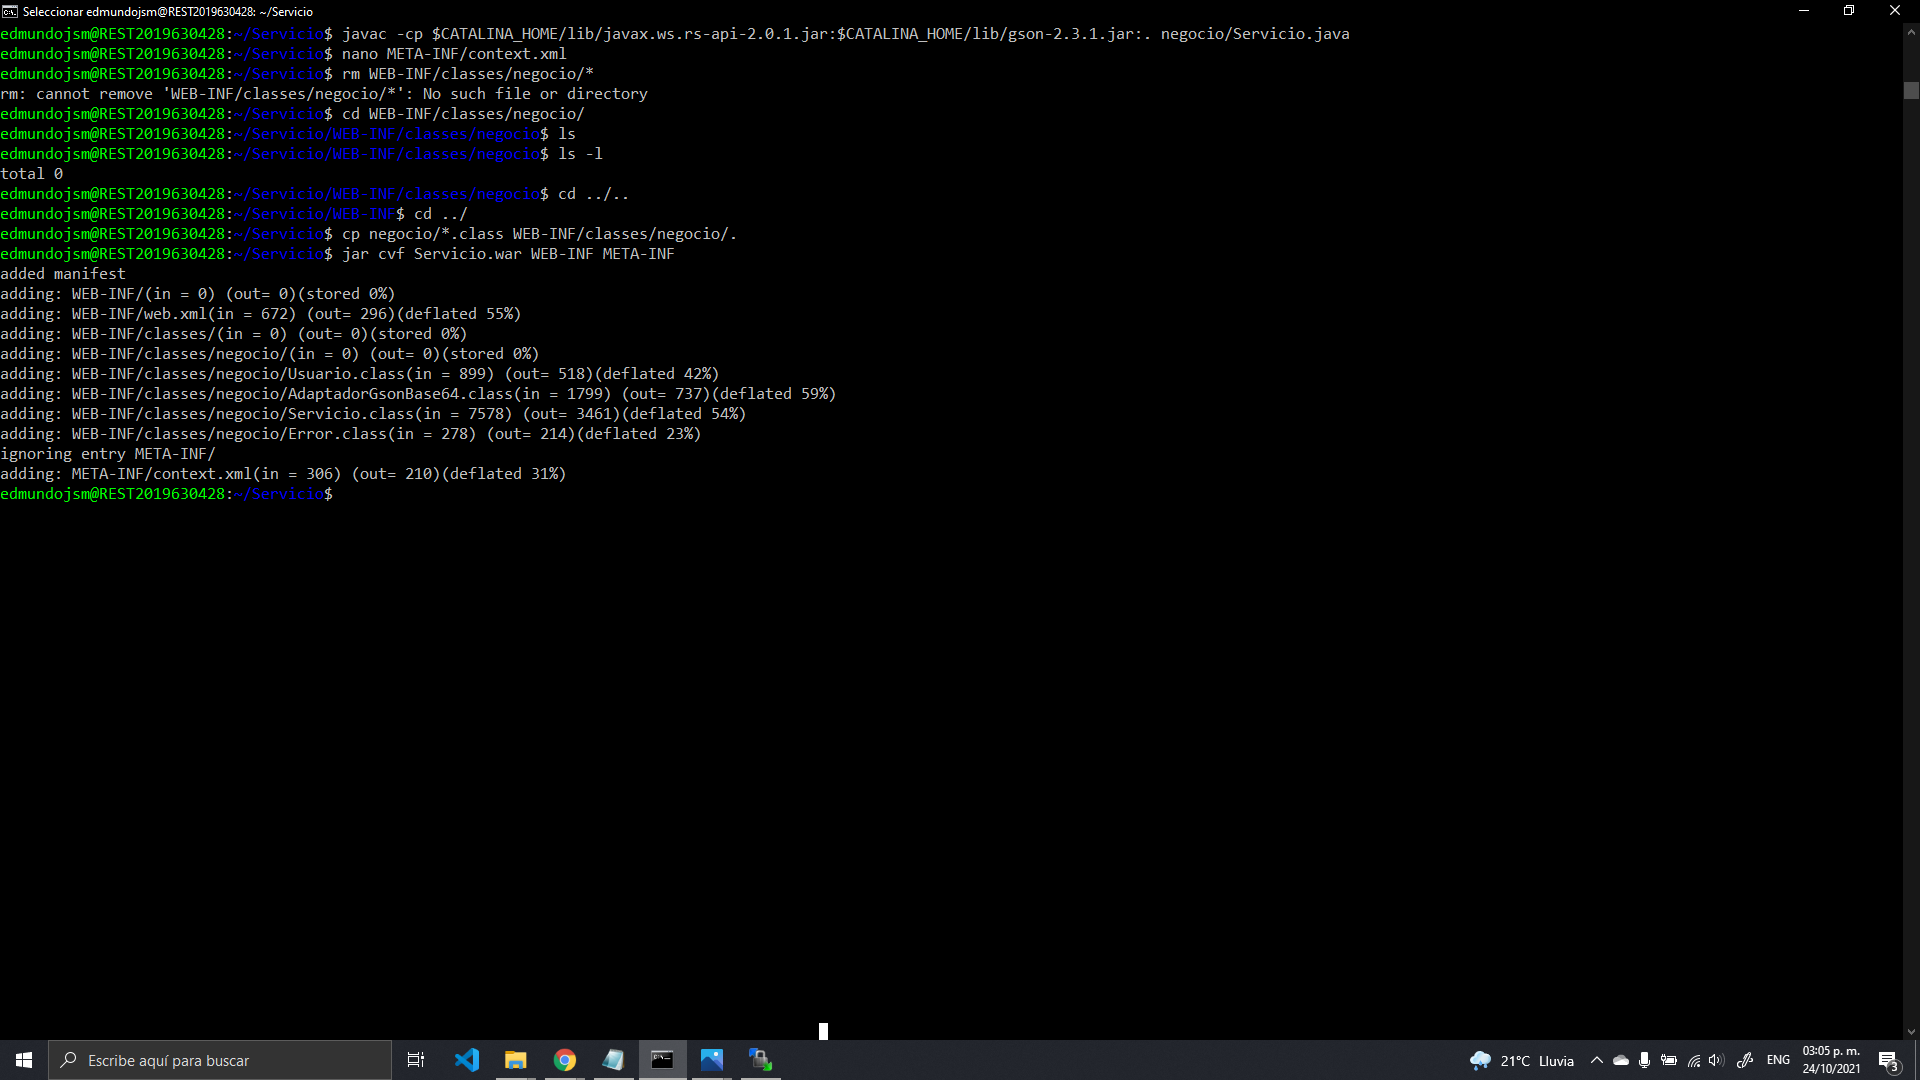
\includegraphics[scale=0.34]{resources/ced6.png}
			\caption{Ejecución de comandos para crear el servicio web para Tomcat .}\label{fig:picture}
		\end{figure}
		\begin{figure}[H]
			\centering
			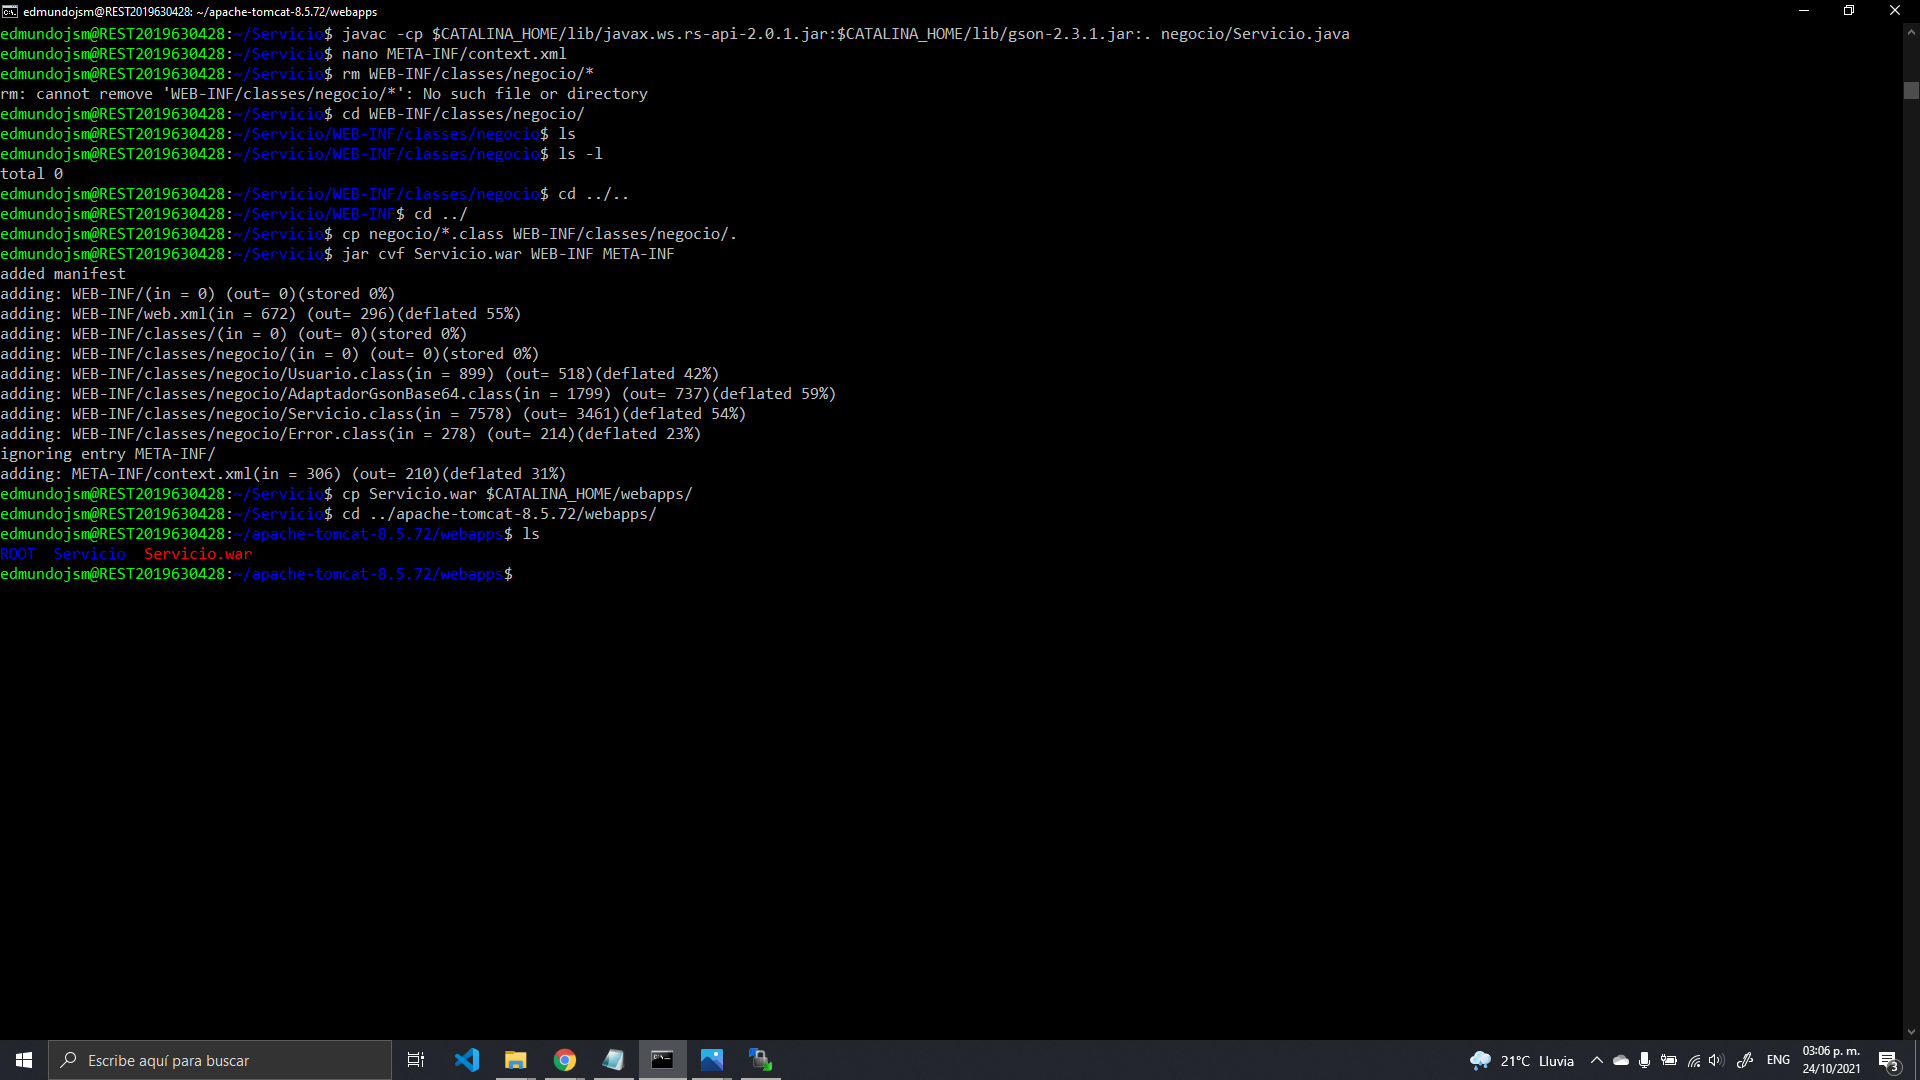
\includegraphics[scale=0.34]{resources/cedF.png}
			\caption{Copia del archivo Servicio.war al directorio webapps de Tomcat, observar que Tomcat desempaca automáticamente los archivos con extensión .war que se encuentran en el directorio webapps.}\label{fig:picture}
		\end{figure}
		\subsection{Prueba del servicio web utilizando HTML-Javascript}
		Antes de ir con las pruebas como tal vamos a pasar los archivos restantes pero primero que nada veremos si Tomcat esta funcionando para ello copiaremos uno de los primeros archivos restantes, el cual sera usuario\_sin\_foto.png a la carpeta ROOT, como vemos en la imagen 37.
		\begin{figure}[H]
			\centering
			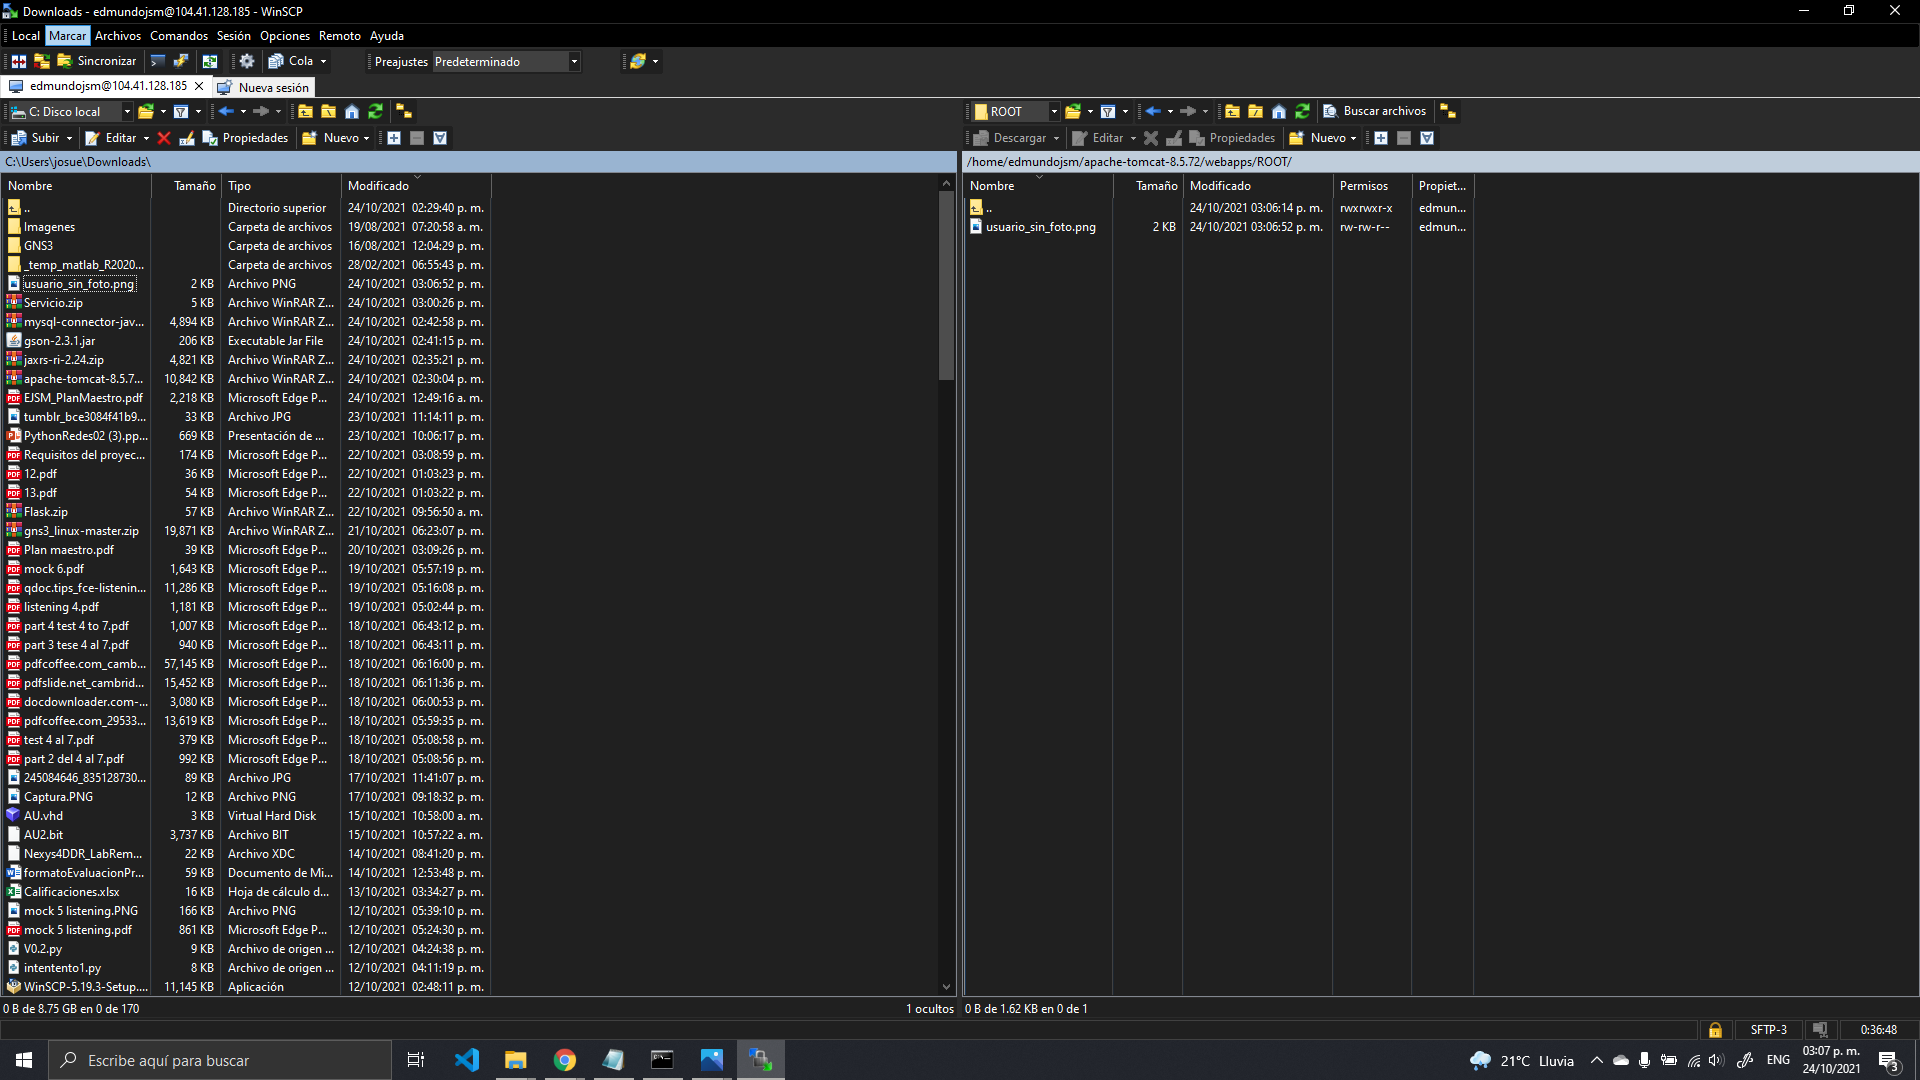
\includegraphics[scale=0.34]{resources/ULTIMO1.png}
			\caption{Copia del archivo usuario\_sin\_foto.png a la carpeta ROOT.}\label{fig:picture}
		\end{figure}
		 Ahora teniendo copiado el archivo no queda mas que probar si funciona correctamente Tomcat como vemos en la figura 38, para ello ingresaremos a la siguiente URL http://104.41.128.185:8080/usuario\_sin\_foto.png mencionar que la IP no es fija, va cambiando de acuerdo a la maquina virtual de cada uno.
		\begin{figure}[H]
			\centering
			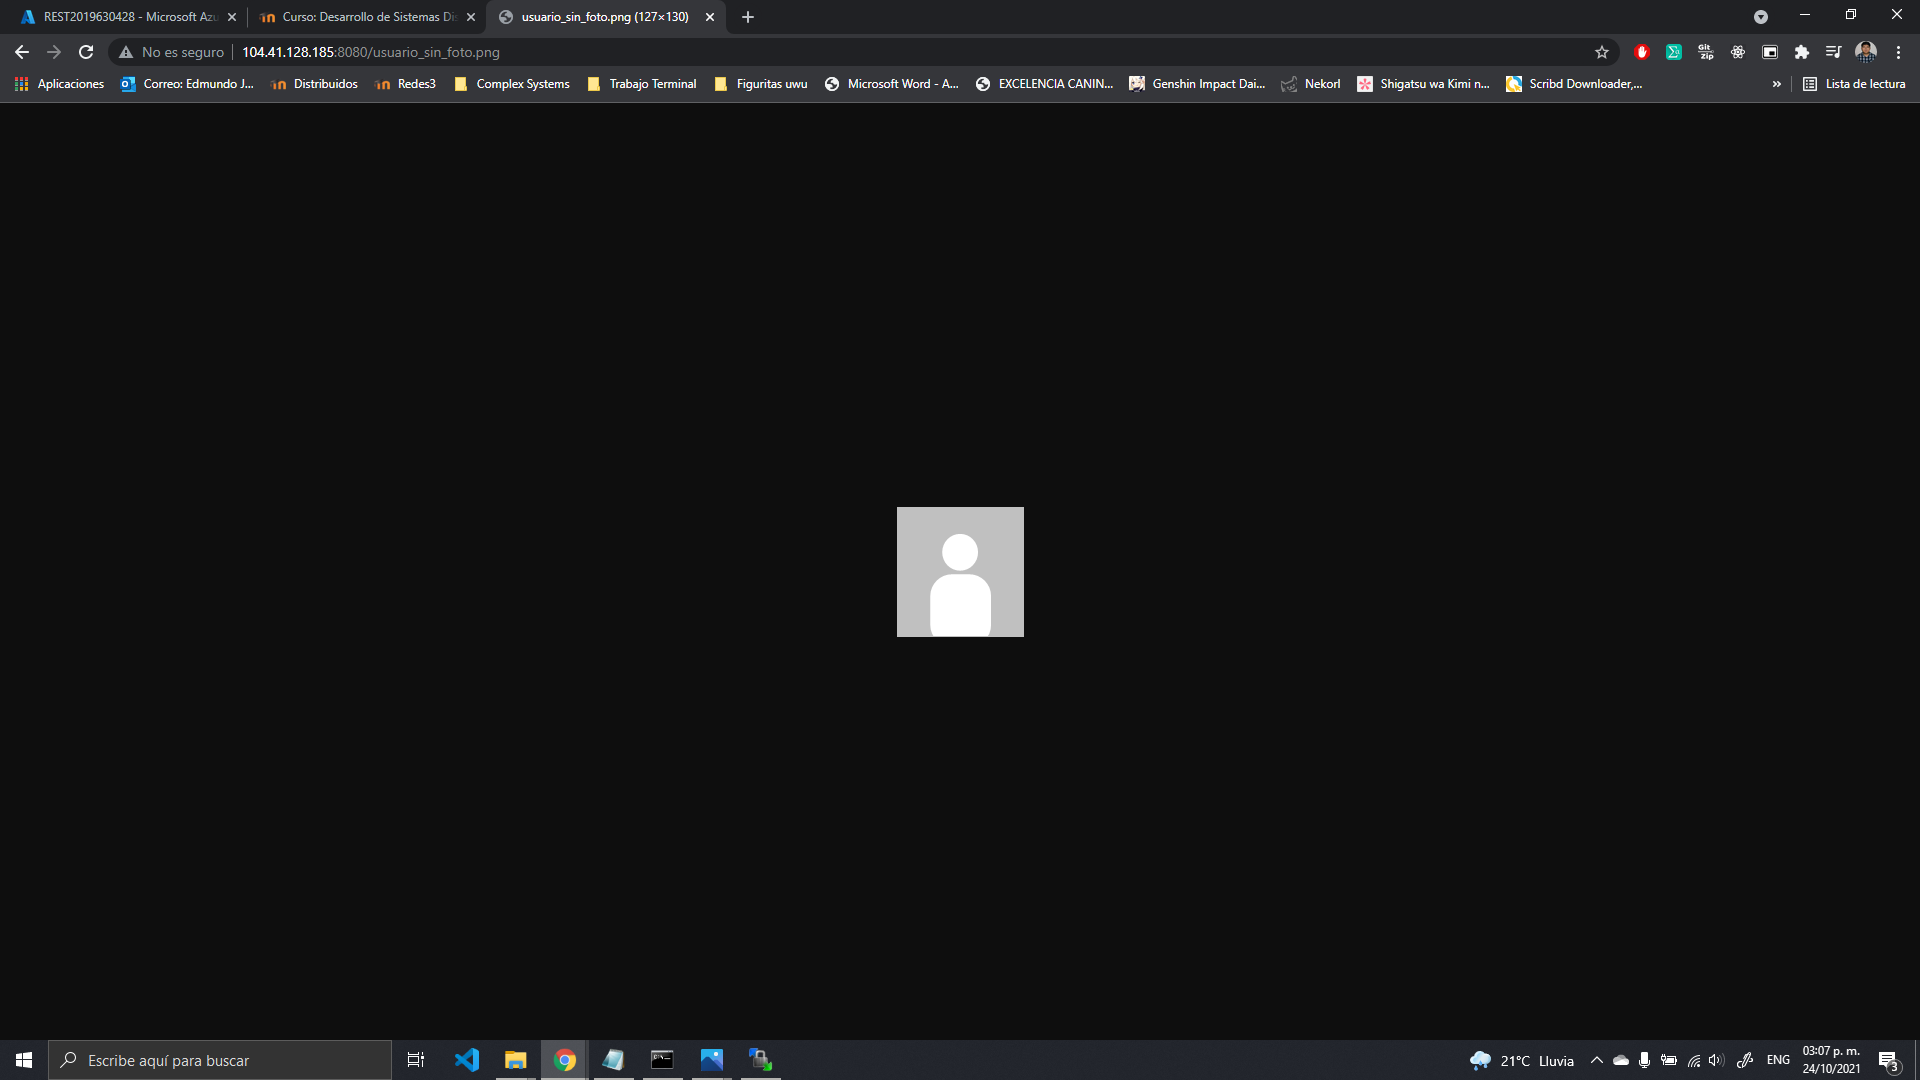
\includegraphics[scale=0.34]{resources/ULTIMO1ok.png}
			\caption{Tomcat funcionando.}\label{fig:picture}
		\end{figure}		 
		 Ahora copiaremos los archivos restantes los cuales son WSClient.js y prueba.html, esto se puede ver en la figura 39.
		 \begin{figure}[H]
			\centering
			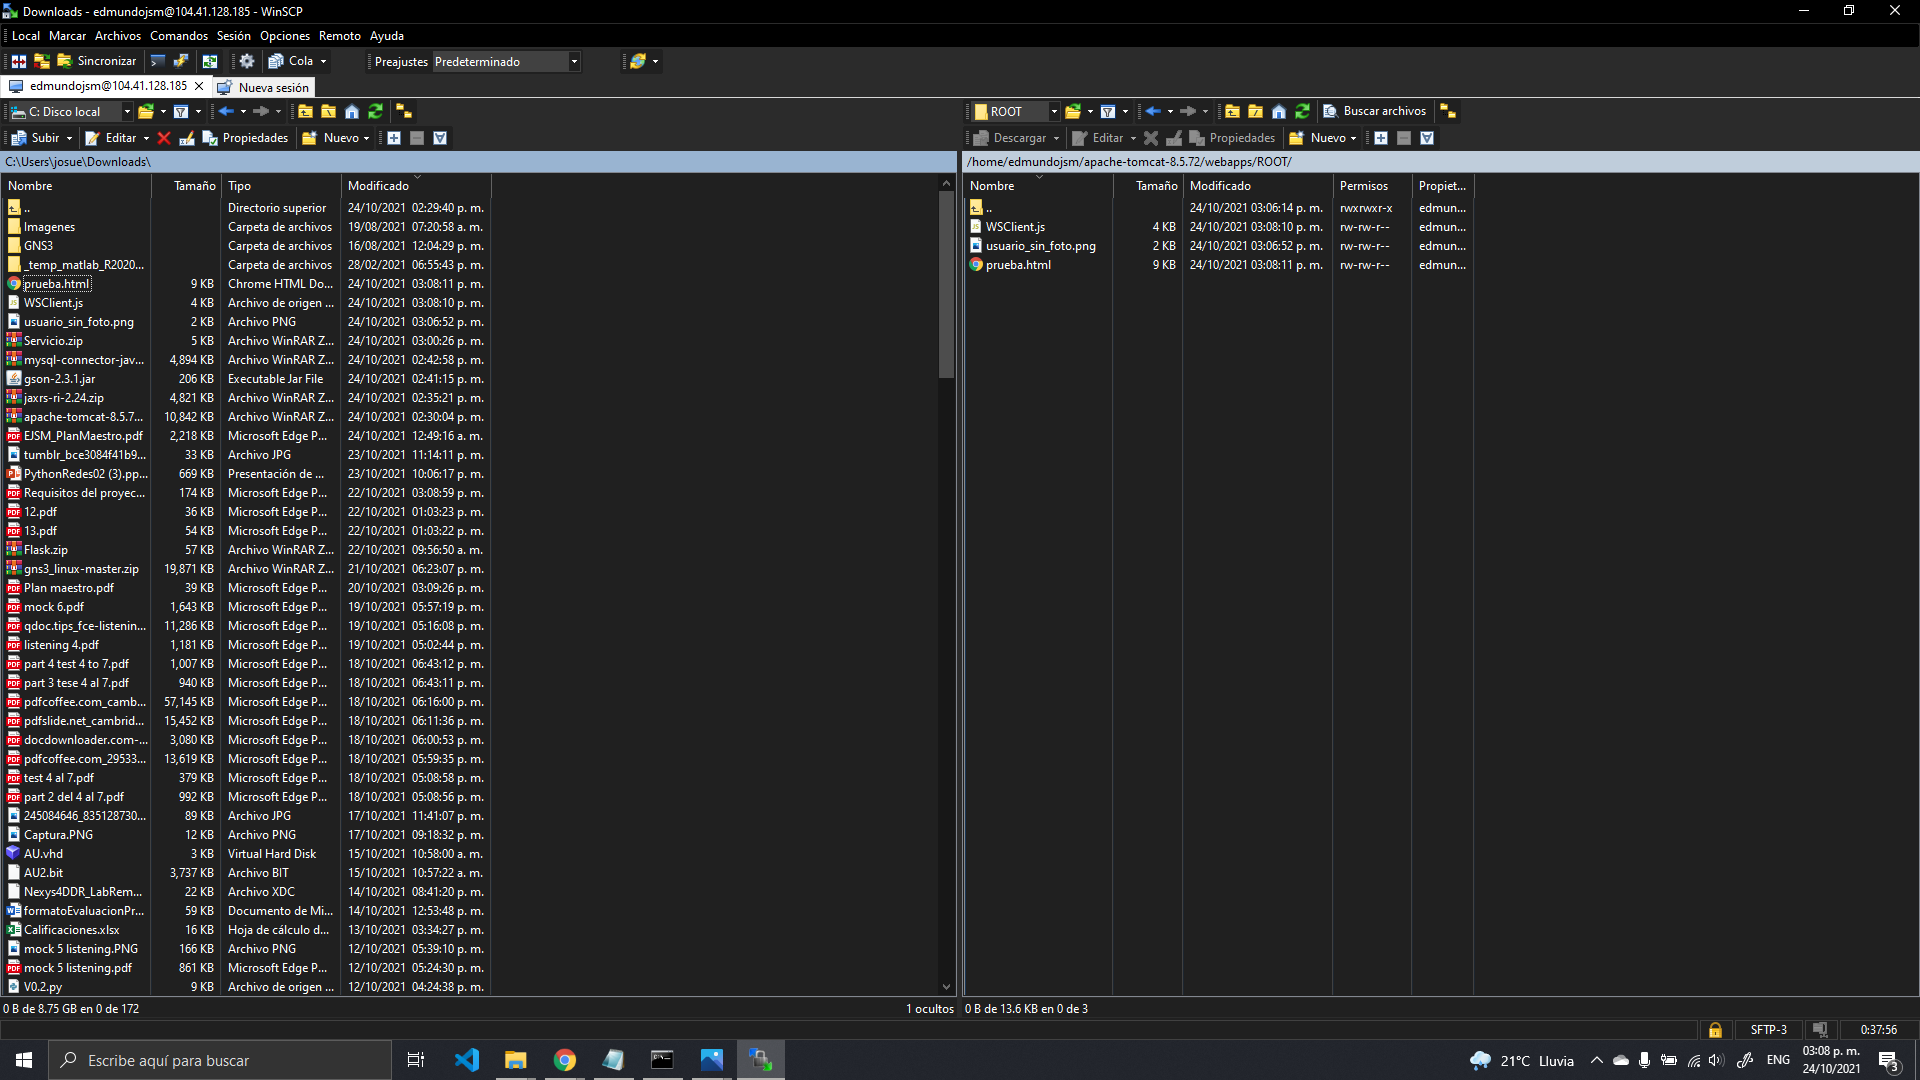
\includegraphics[scale=0.34]{resources/ULTIMO2y3.png}
			\caption{Copia de los archivos WSClient.js y prueba.html a la maquina virtual.}\label{fig:picture}
		\end{figure}
		Ahora vayamos netamente a las pruebas. Para empezar nos dirigiremos a la URL http://104.41.128.185:
8080/prueba.html (ver imagen 40) esto para cargar una pagina HTML en la cual podemos hacer el clásico ABCC, es decir altas, bajas, cambios y consultas de una base de datos. Empecemos así con una alta, para esto veamos la figura 41, en la figura 40 vemos los datos que serán dados de alta y en la figura 5 vemos el mensaje de que el usuario se dio de alta.
		\begin{figure}[H]
			\centering
			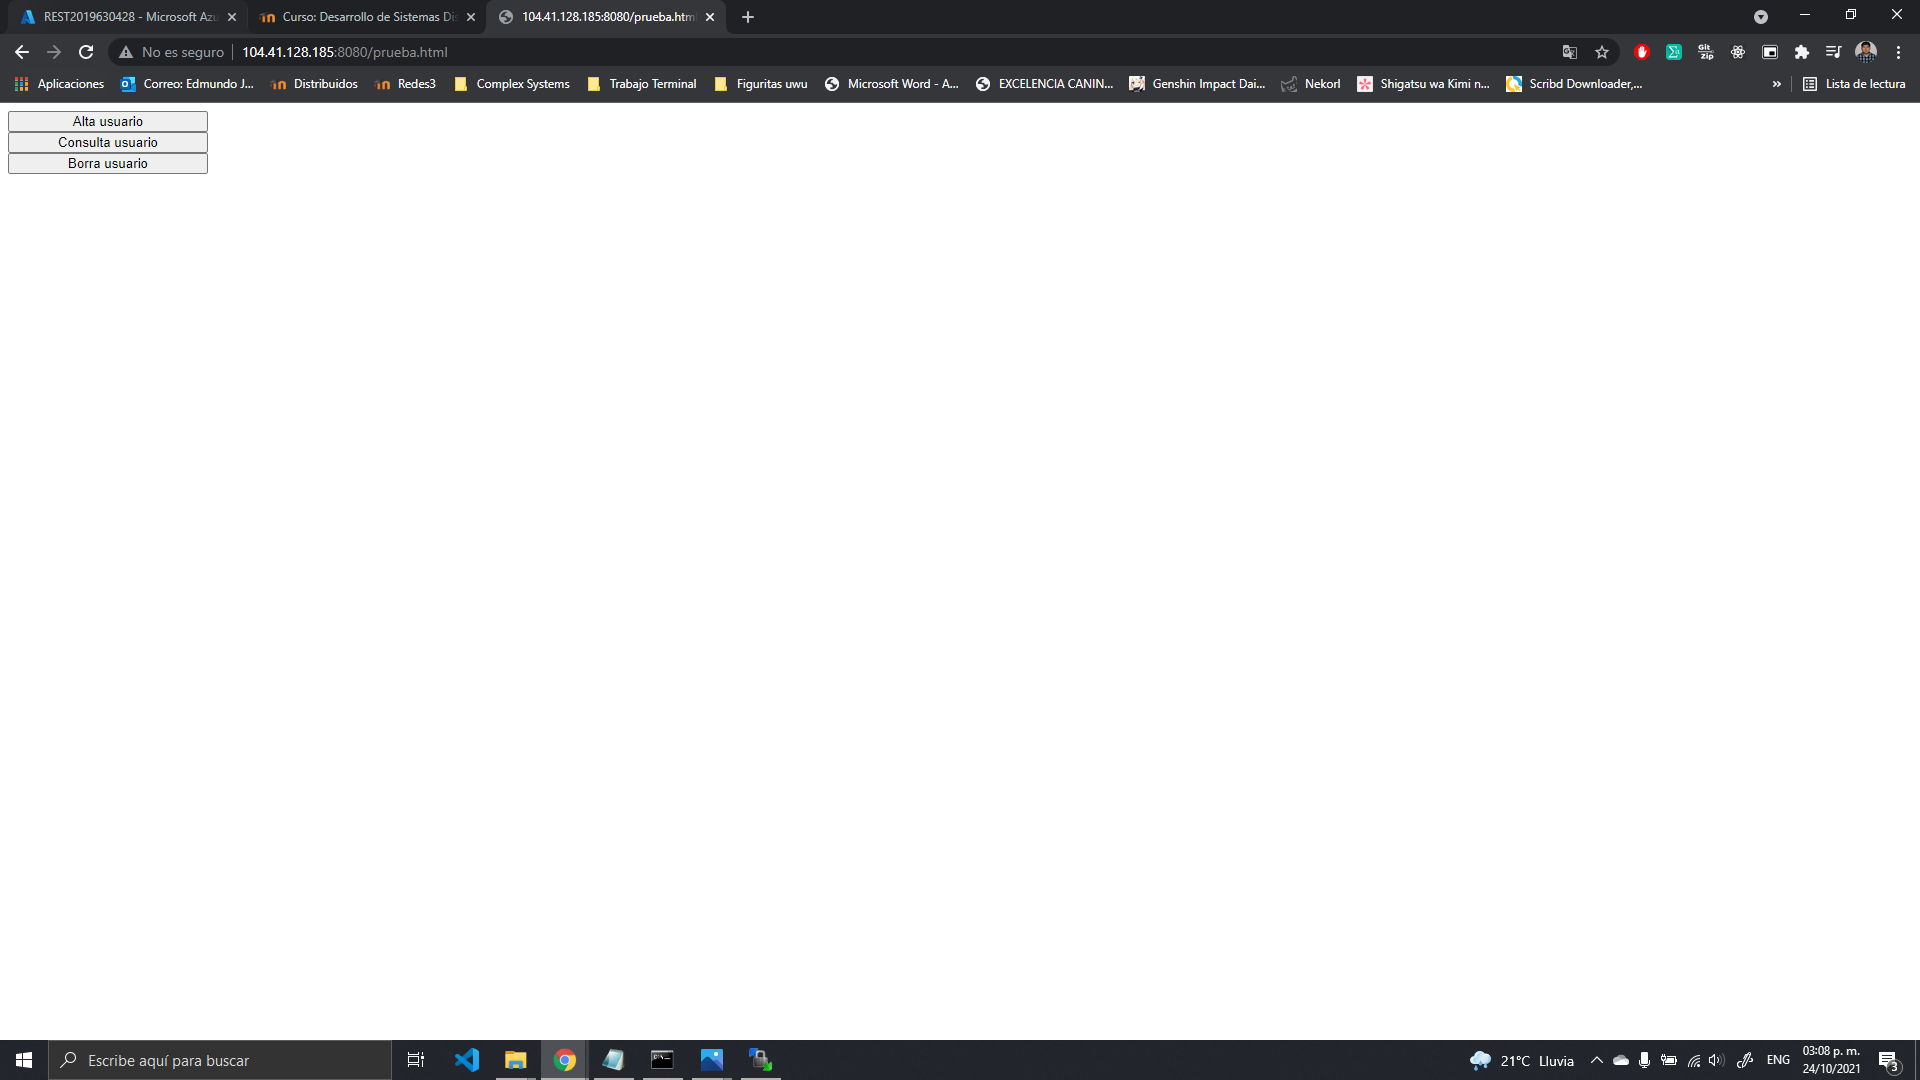
\includegraphics[scale=0.34]{resources/ULTIMO4.png}
			\caption{Pagina prueba.html.}\label{fig:picture}
		\end{figure}
		\begin{figure}[H]
			\centering
			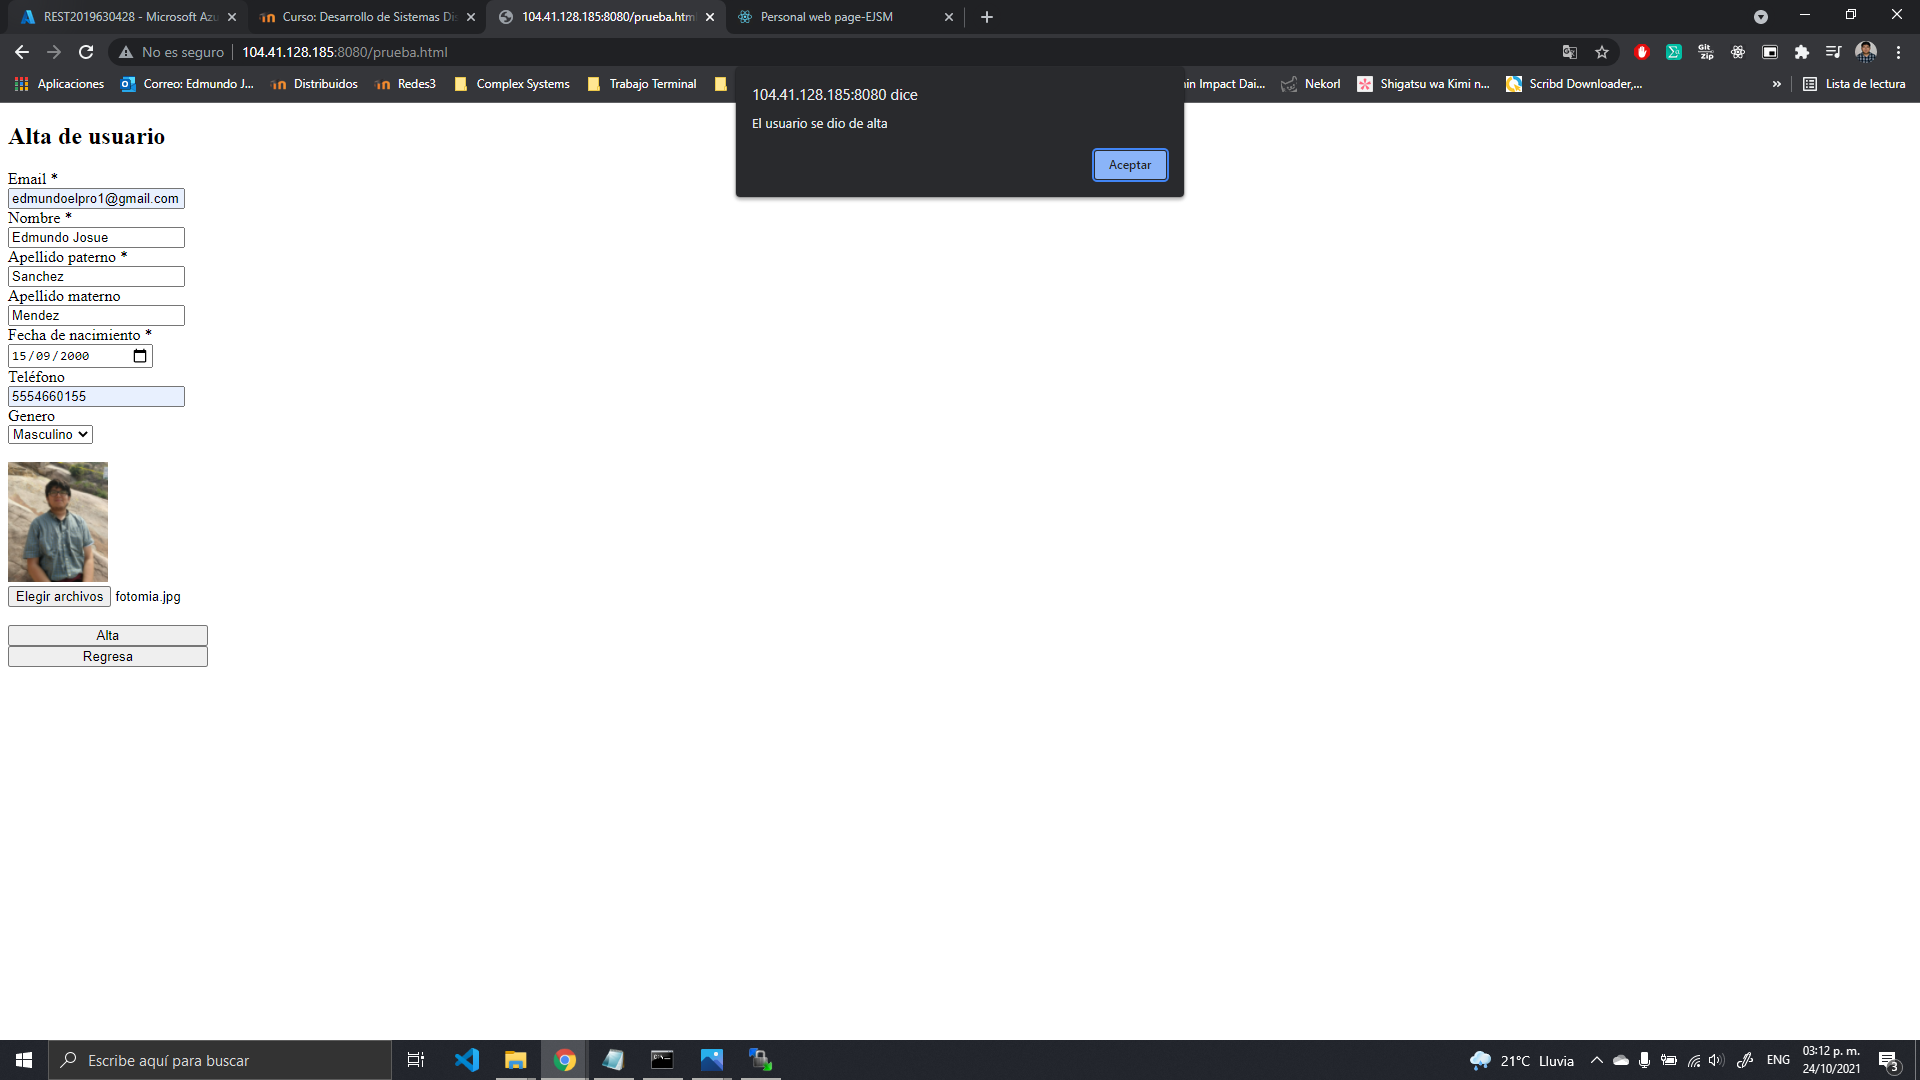
\includegraphics[scale=0.34]{resources/ULTIMO5.png}
			\caption{Alta de usuario.}\label{fig:picture}
		\end{figure}
		La siguiente prueba sera dar de alta un usuario con el mismo correo que se ocupo, como vemos nos regresa un mensaje diciendo que el email ya existe como se ve en la figura 42.
		\begin{figure}[H]
			\centering
			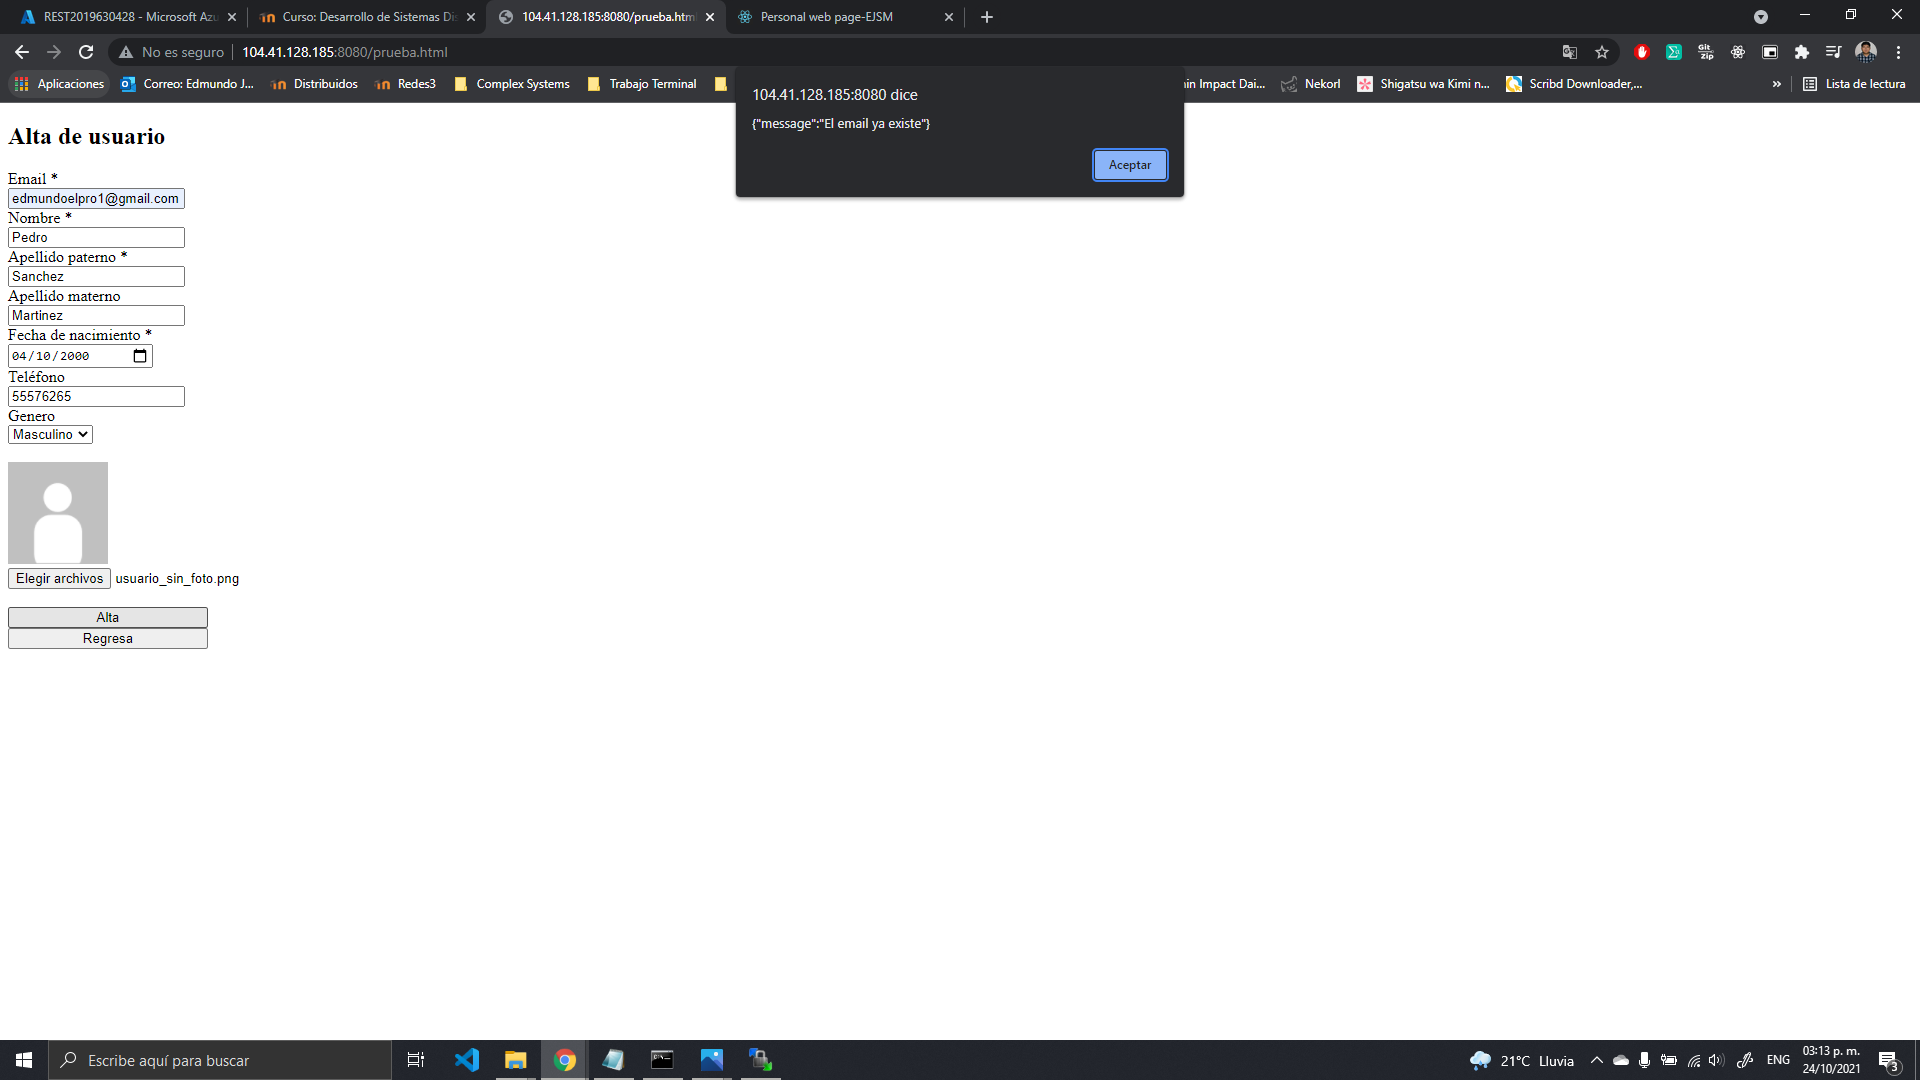
\includegraphics[scale=0.34]{resources/ULTIMO6.png}
			\caption{Alta de usuario con el mismo correo.}\label{fig:picture}
		\end{figure} 
		Una prueba mas sera la de consultar un usuario por medio del correo electrónico como vemos en la figura 43 solo colocamos el correo electrónico que se registro y como vemos en la figura 44 nos muestra la información que registramos en la figura 41.
		\begin{figure}[H]
			\centering
			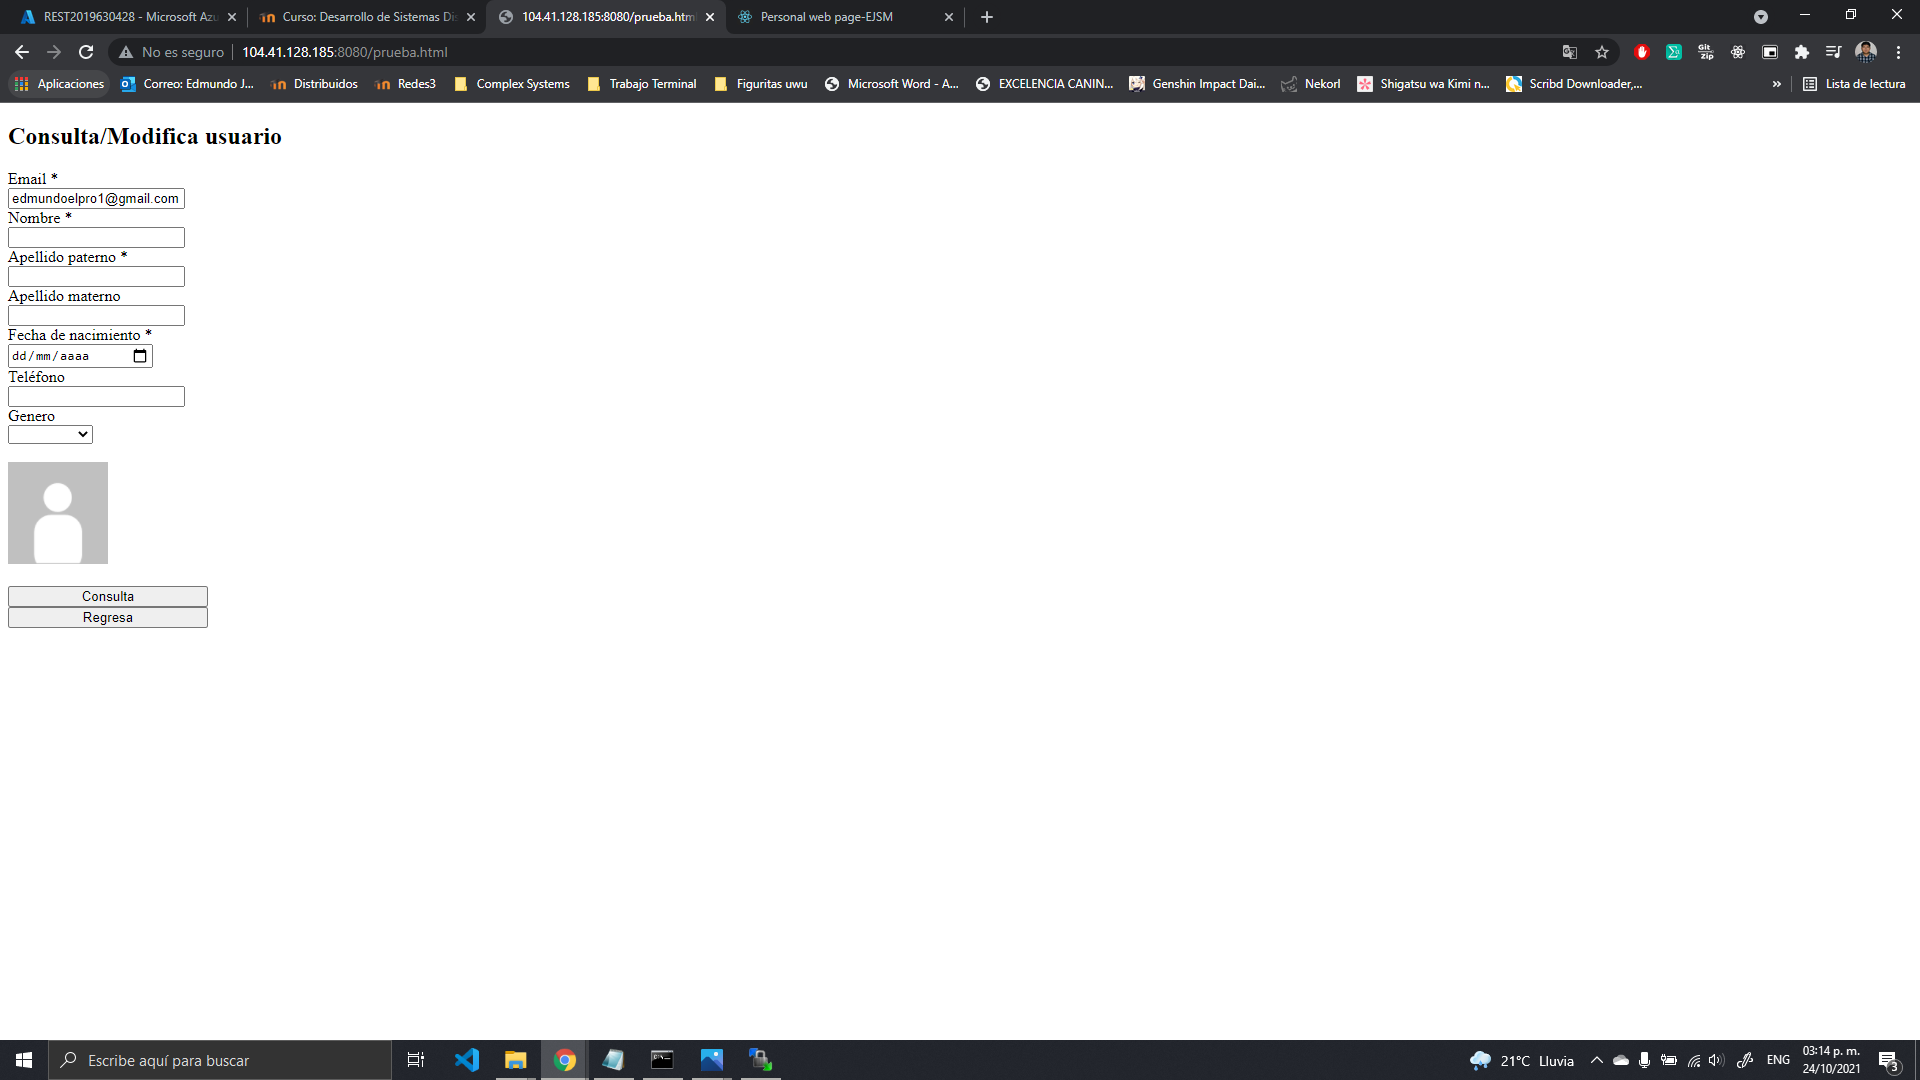
\includegraphics[scale=0.34]{resources/ULTIMO7.1.png}
			\caption{Consulta por medio del correo.}\label{fig:picture}
		\end{figure}
		\begin{figure}[H]
			\centering
			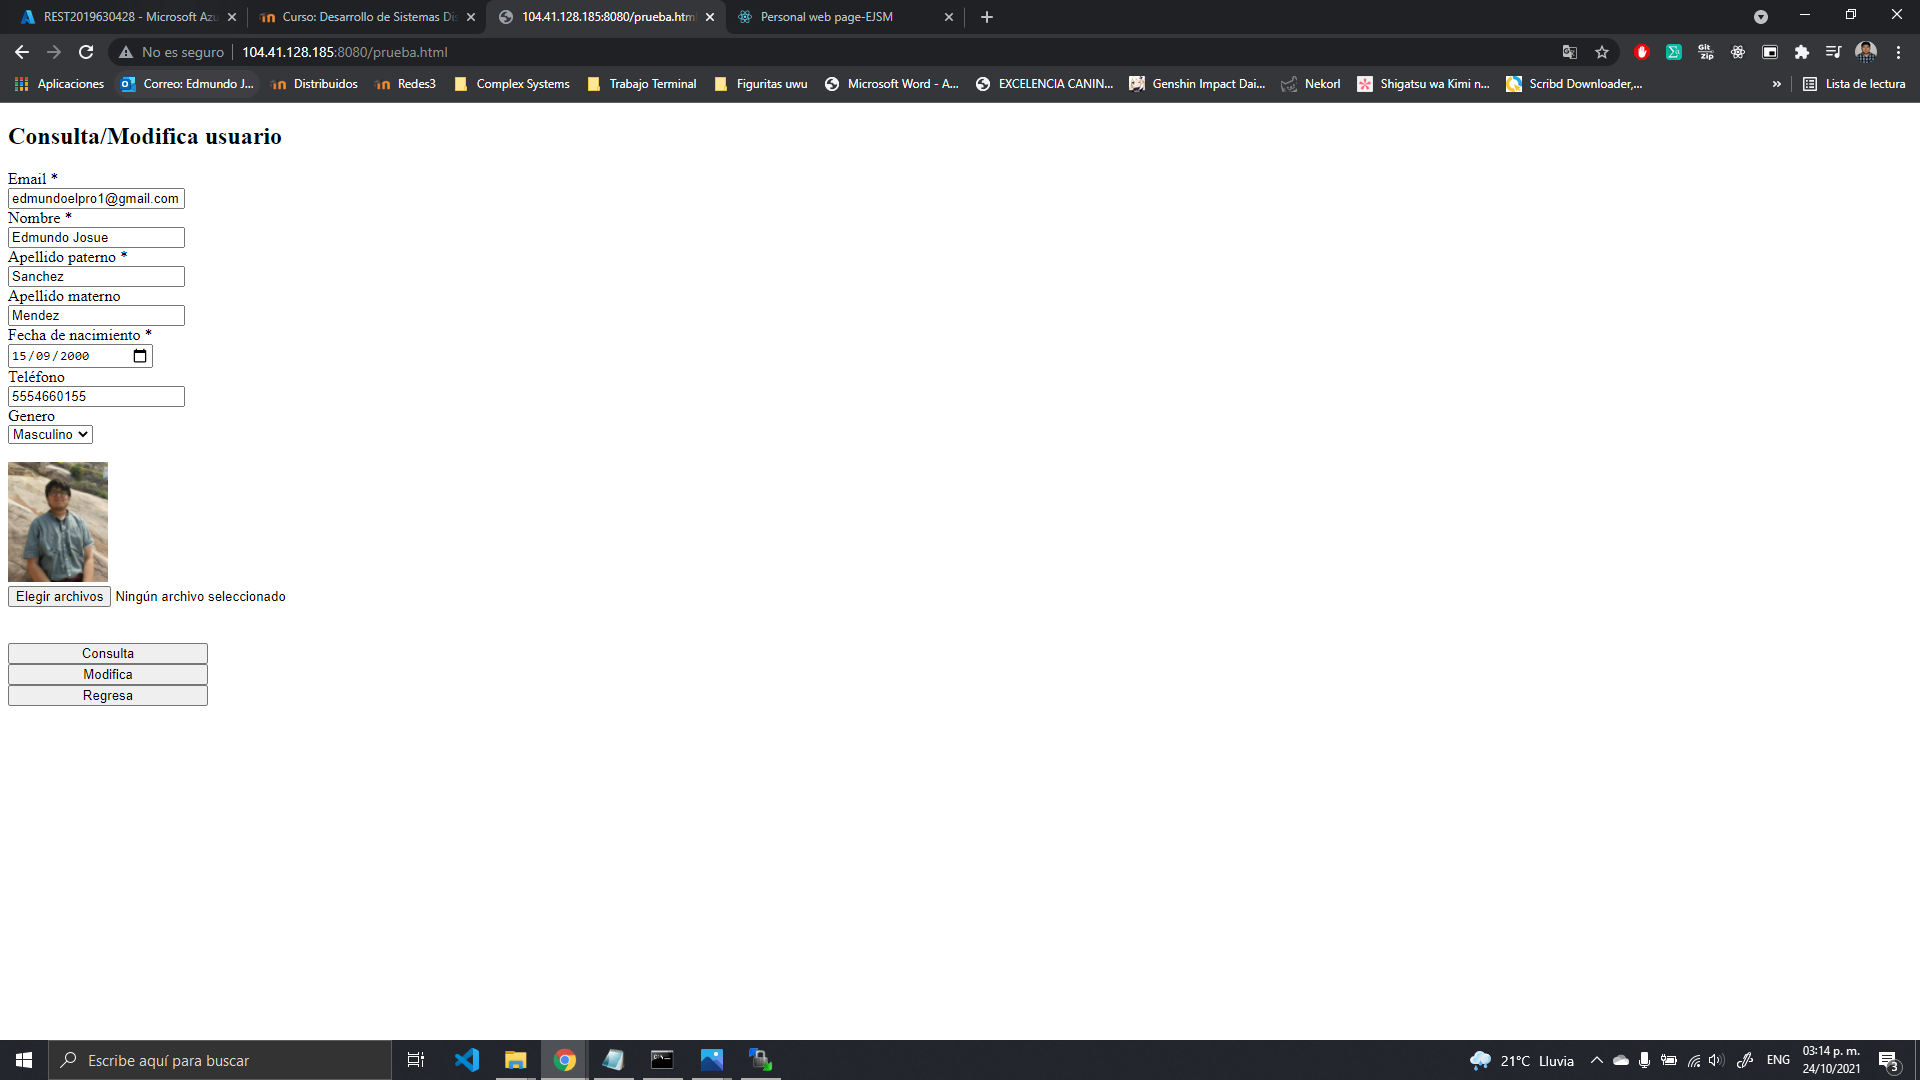
\includegraphics[scale=0.34]{resources/ULTIMO7.2.png}
			\caption{Resultado de la consulta anterior.}\label{fig:picture}
		\end{figure}
		Como penúltima prueba sera modificar el usuario anteriormente registrado, en este caso solo modificamos la fecha de nacimiento y el teléfono para esto podemos ver la figura 45 y que nos devuelve un mensaje con el contenido ''El usuario se modificó" y como vemos en la figura 46 al consultar el usuario tiene la información actualizada.
		\begin{figure}[H]
			\centering
			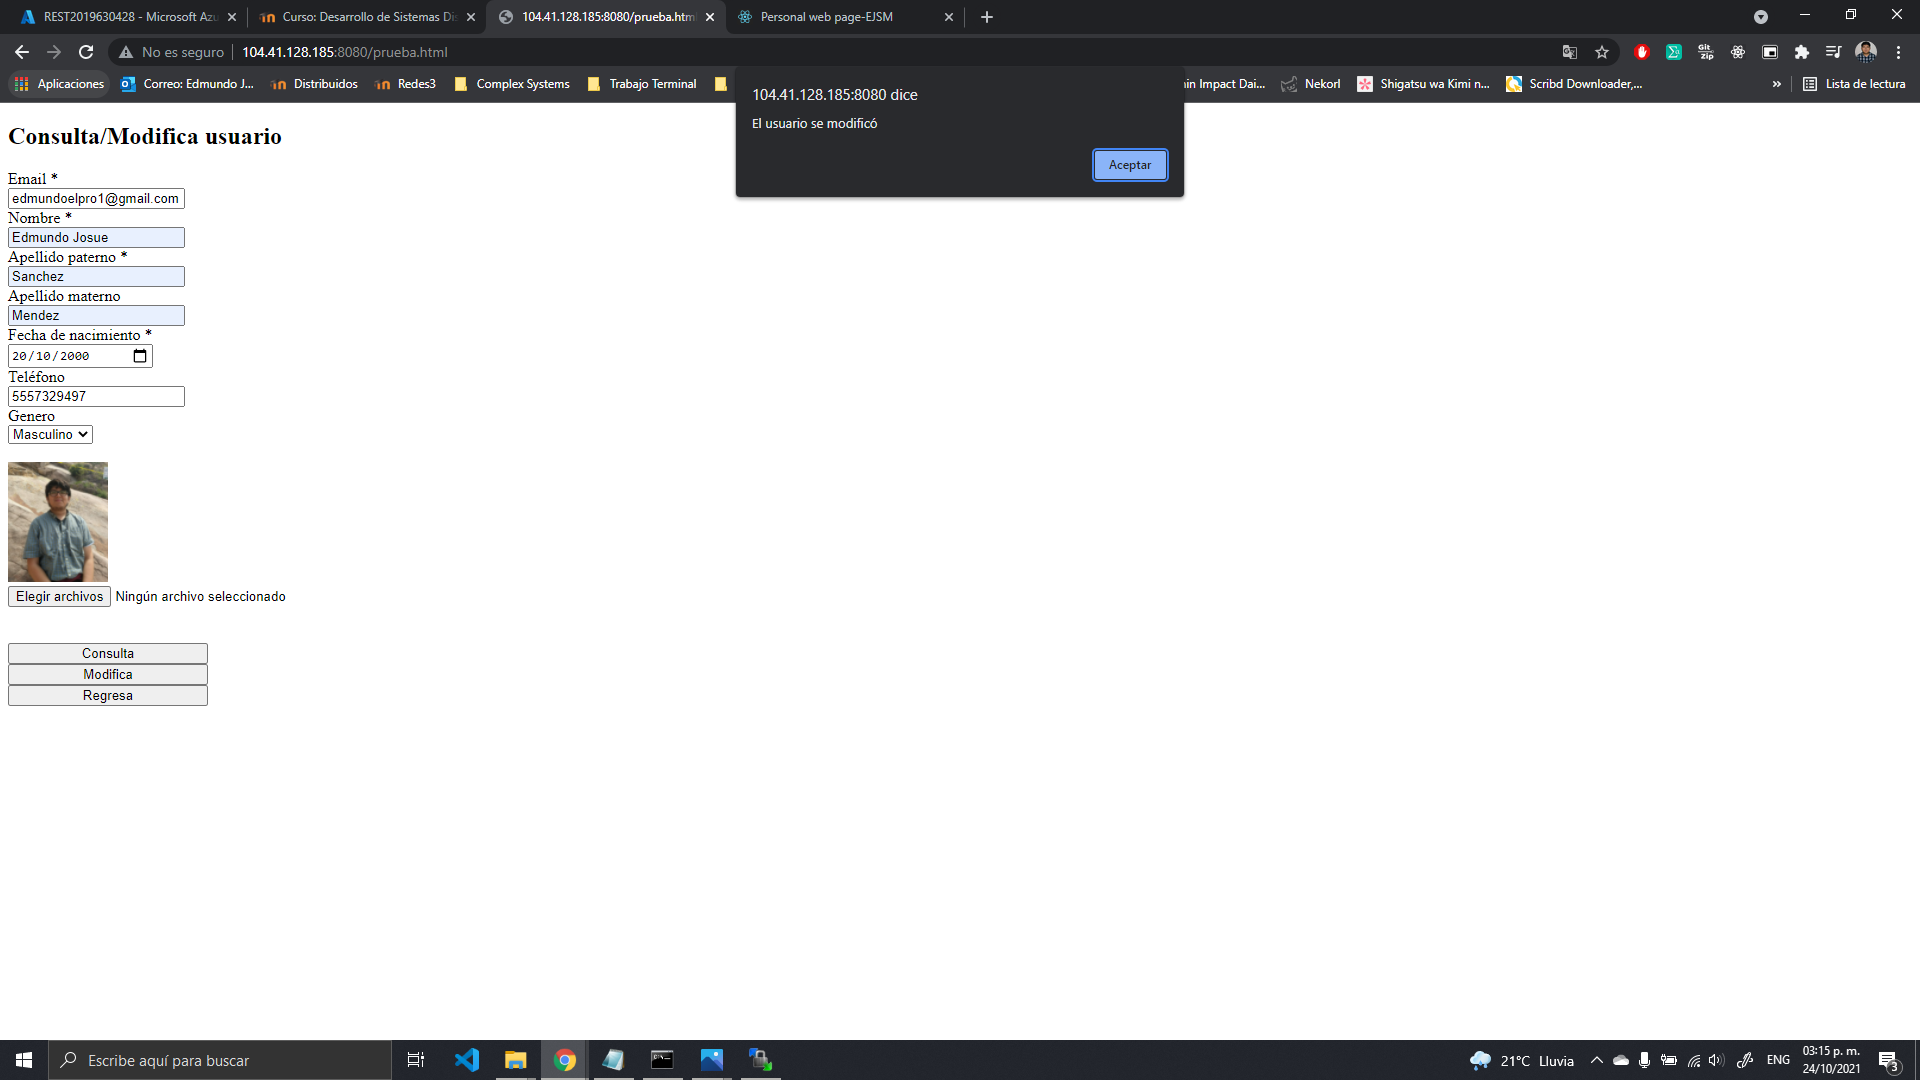
\includegraphics[scale=0.34]{resources/ULTIMO8.png}
			\caption{Cambio en la información del usuario.}\label{fig:picture}
		\end{figure}
		\begin{figure}[H]
			\centering
			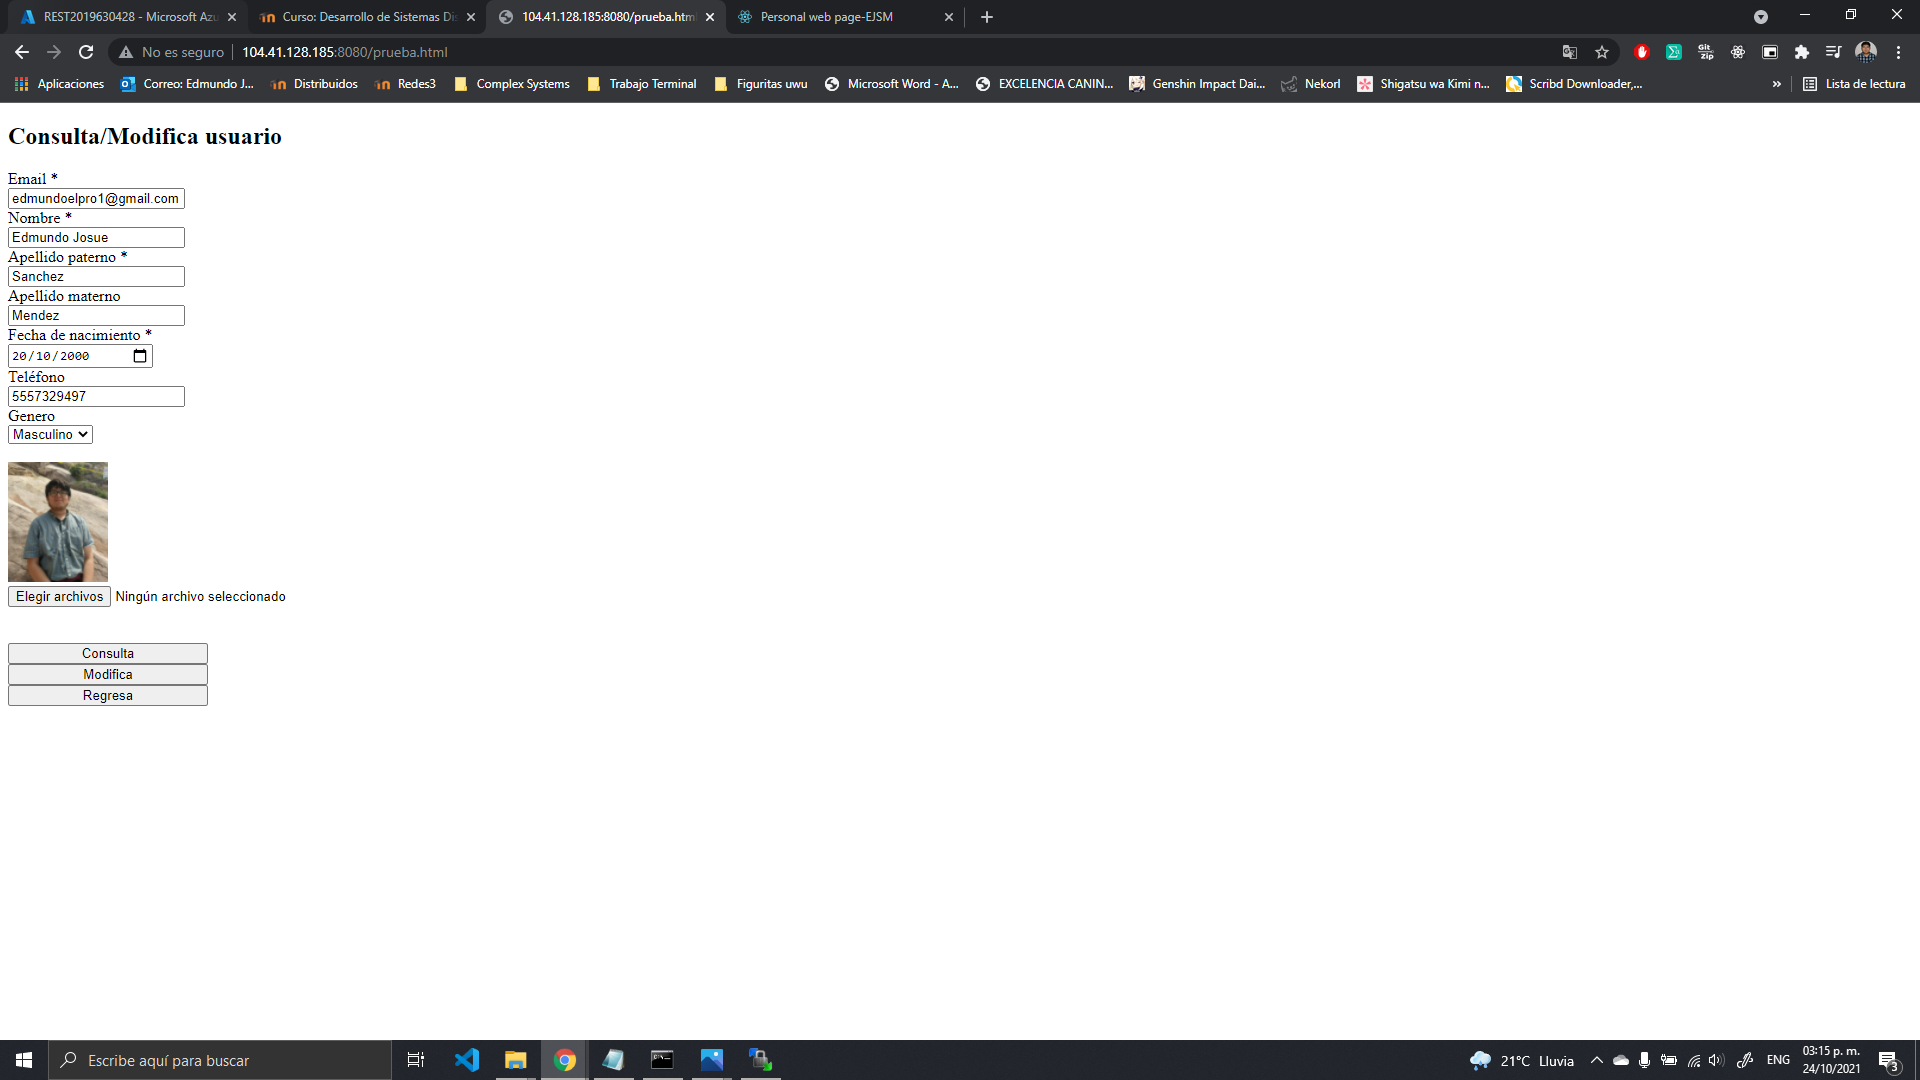
\includegraphics[scale=0.34]{resources/ULTIMO9.png}
			\caption{Resultado del cambio realizado.}\label{fig:picture}
		\end{figure}
		Como ultima prueba borraremos el usuario registrado por medio del correo que se registro, como vemos en la figura 47 nos arroja un mensaje con el contenido "El usuario se borro" y en la figura 48 vemos como al querer consultar después de que el usuario fue borrado nos arroja un mensaje de error diciendo que el email no existe.
		\begin{figure}[H]
			\centering
			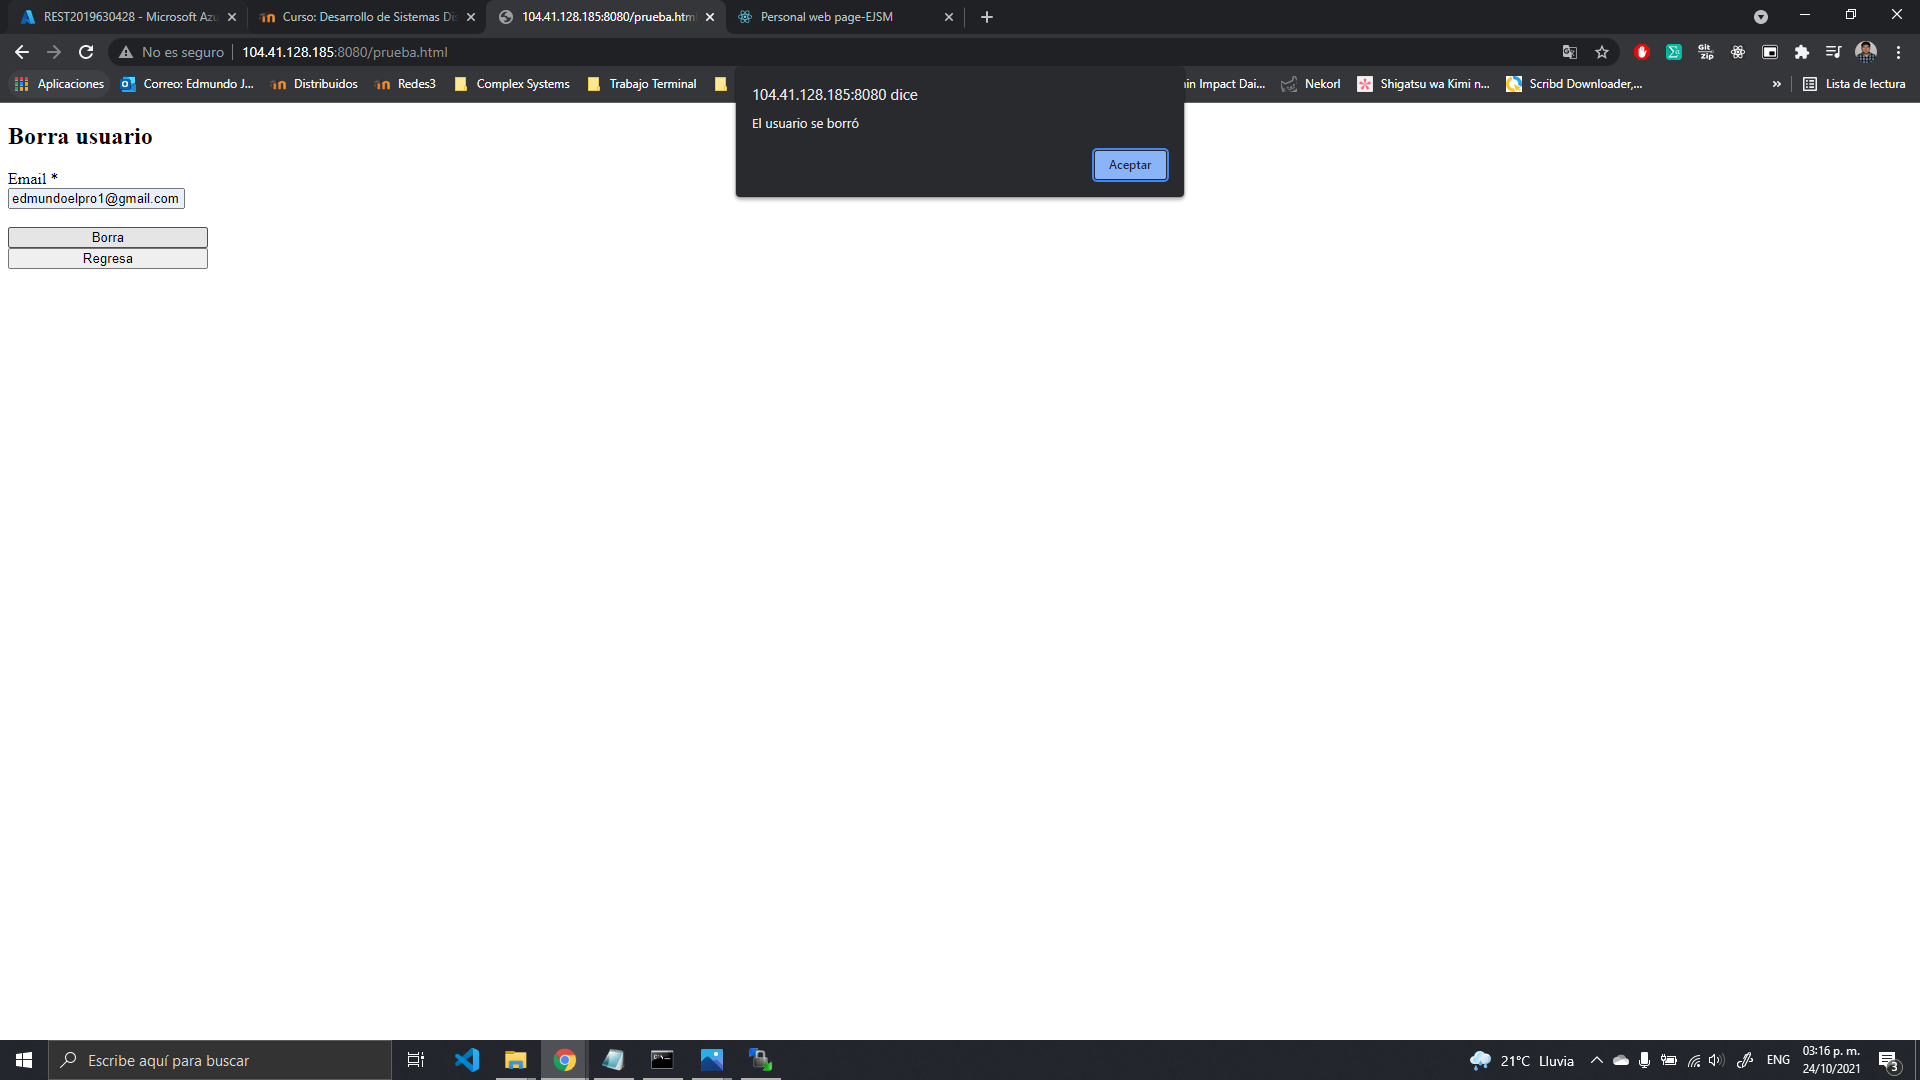
\includegraphics[scale=0.34]{resources/ULTIMO10.png}
			\caption{Eliminación del usuario.}\label{fig:picture}
		\end{figure}
		\begin{figure}[H]
			\centering
			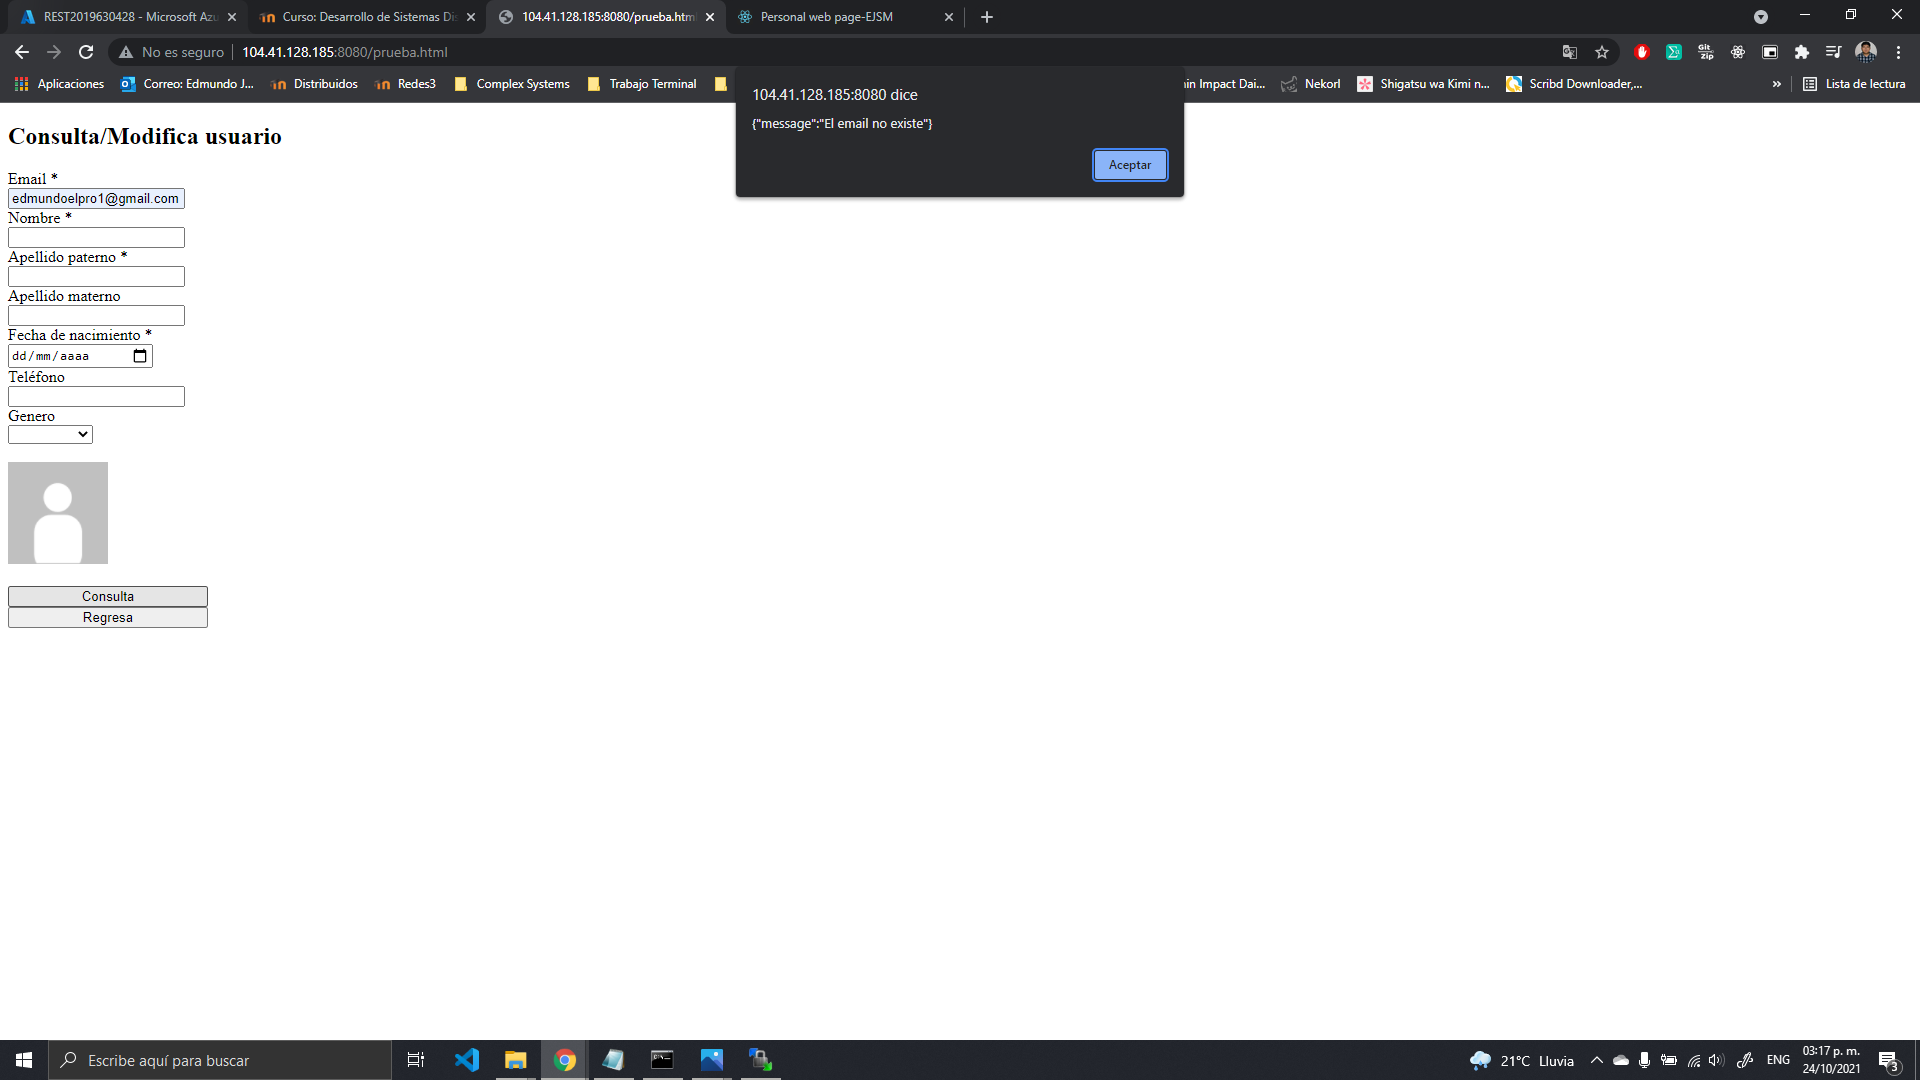
\includegraphics[scale=0.34]{resources/ULTIMO10OK.png}
			\caption{Consulta del usuario borrado en la figura anterior.}\label{fig:picture}
		\end{figure}
		Finalmente haremos las mismas pruebas realizadas pero desde un teléfono inteligente, el orden sera el mismo que las pruebas anteriores, solo que esta vez no detallare mucho, sin embargo, cada imagen tendrá lo que ahí se hizo.
		\begin{figure}[H]
			\centering
			\includegraphics[scale=0.18]{resources/Screenshot_20211024-152136.png}
			\caption{Pagina prueba.html.}\label{fig:picture}
		\end{figure}
		\begin{figure}[H]
			\centering
			\includegraphics[scale=0.18]{resources/Screenshot_20211024-152129.png}
			\caption{Alta de usuario.}\label{fig:picture}
		\end{figure}
		\begin{figure}[H]
			\centering
			\includegraphics[scale=0.18]{resources/Screenshot_20211024-152206.png}
			\caption{Consulta de usuario.}\label{fig:picture}
		\end{figure}
		\begin{figure}[H]
			\centering
			\includegraphics[scale=0.18]{resources/Screenshot_20211024-152418.png}
			\caption{Modificación de usuario.}\label{fig:picture}
		\end{figure}
		\begin{figure}[H]
			\centering
			\includegraphics[scale=0.18]{resources/Screenshot_20211024-152450.png}
			\caption{Nueva información de usuario.}\label{fig:picture}
		\end{figure}
		\begin{figure}[H]
			\centering
			\includegraphics[scale=0.18]{resources/Screenshot_20211024-152508.png}
			\caption{Baja de usuario.}\label{fig:picture}
		\end{figure}
		\begin{figure}[H]
			\centering
			\includegraphics[scale=0.18]{resources/Screenshot_20211024-152533.png}
			\caption{Consulta de usuario después de borrarlo.}\label{fig:picture}
		\end{figure}
		Como vemos podemos usar este servicio tanto en una computadora de escritorio o laptop como en un dispositivo inteligente, ya sea una tableta o un celular.
		\subsection{Creación de una imagen de la maquina virtual conservando el usuario}
		En este punto tendremos que crear una imagen de la maquina virtual ya que esta tendrá todo lo que instalamos y usamos para esta practica, esto se hace con el fin de usar la imagen para las tareas posteriores, este proceso lo vemos en las figuras 56 a la 59.
		\begin{figure}[H]
			\centering
			\includegraphics[scale=0.34]{resources/imagenvm1.png}
			\caption{Ejecucion del comando sudo waagent -deprovision, esto para crear la imagen con todo y el usuario.}\label{fig:picture}
		\end{figure}
		\begin{figure}[H]
			\centering
			\includegraphics[scale=0.34]{resources/imagenvm2.png}
			\caption{Opción seleccionada de eliminar automáticamente esta maquina virtual después de crear la imagen, también elegimos un nombre el cual es APACHEMYSQL, indicando que tenemos instalado Tomcat y MySQL.}\label{fig:picture}
		\end{figure}
		\begin{figure}[H]
			\centering
			\includegraphics[scale=0.34]{resources/imagenvm3.png}
			\caption{Información de la imagen.}\label{fig:picture}
		\end{figure}
		\begin{figure}[H]
			\centering
			\includegraphics[scale=0.34]{resources/imagenvOK.png}
			\caption{Imagen creada de manera exitosa.}\label{fig:picture}
		\end{figure}
		\section{Conclusiones}
	En esta practica observamos el funcionamiento de una aplicación REST, y su comportamiento básico. El uso de una maquina virtual y que a su vez este montado en un servidor web Tomcat nos hace ver como el sistema distribuido como una sola aplicación que esta siendo ejecutado en consola con el SO Linux, también, podemos ver el uso de algo conocido en el desarrollo de aplicación web como back-end ya que usamos MySQL como el manejador de base de datos y compilando el programa con JDBC para poder tener la conexión con la base de datos y haciendo uso de Java para la comunicación, por otro lado el front-end que es lo que se muestra al usuario final, muestra la aplicación con una interfaz y su interacción con el back-end.
\end{document}
